\chapter{Correction en énergie des jets à l'aide d'événements \texorpdfstring{$\Pphoton$}{γ} + jets} \label{chap:jetmet}

\begin{fmffile}{chapitre4}

Comme on a pu le voir au chapitre précédent, les algorithmes de reconstruction des jets sont complexes : ils opèrent sur une liste d'objets et les agglomèrent s'ils respectent certaines conditions (voir \cref{sec:jet_reco}). Les propriétés du jet (énergie, impulsion, charge, etc.) sont ainsi déterminées grâce à ces constituants. Ainsi, s'il en manque certains, ou si leurs énergies sont mal déterminées, les propriétés du jet seront impactées.

\smallskip

C'est pourquoi on applique aux jets toute une série de corrections, destinées à corriger ces effets. Les différentes étapes de correction sont détaillées dans ce chapitre.

\section{Les différents niveaux de corrections}

Plusieurs effets sont à prendre en compte lorsque l'on veut corriger l'énergie des jets. En effet, la réponse des sous-détecteurs peut varier selon plusieurs facteurs, tels que la présence de \pu, la position angulaire et l'impulsion transverse des particules, le type de particule, ...

CMS a adopté une approche factorisée afin de corriger convenablement ces effets. Plusieurs niveaux de corrections sont ainsi définis, chacun corrigeant un effet particulier. Chaque niveau dépend des corrections appliquées au niveau précédent, et l'ordre dans lequel sont appliqués ces corrections est donc important. On compte trois niveaux de corrections différents :

\begin{description}
    \item[Niveau 1] Ce niveau de correction corrige les effets du \pu et du bruit des détecteurs.
    \item[Niveau 2 et 3] Ces niveaux permettent de corriger les variation d'efficacité de la reconstruction des jets, en fonction de l'angle et l'impulsion transverse des jets.
\end{description}

Ces corrections sont appliquées à la fois aux données collectées et à la simulation. Néanmoins, il est apparu que la simulation ne reproduisait pas (encore) parfaitement la réalité. Il a donc été décidé d'ajouter un quatrième niveau de corrections, nommé corrections résiduelles, appliqué uniquement aux données, qui permet de corriger des dernières différences qui subsistent entre données et simulation.

\medskip

Chaque niveau est décrit en détails ci-dessous.

\subsection[Les corrections de niveau 1]{Les corrections de niveau 1 \citep{1748-0221-6-11-P11002}} \label{sec:jec_l1}

On a déjà vu lors du \cref{chap:detecteur} que le \pu entraînait une activité supplémentaire dans le détecteur. Cela se traduit directement par une augmentation de l'énergie des jets reconstruits, puisque certaines particules agglomérées au sein d'un jet proviennent en réalité des interactions parasites plutôt que de l'événement dur.

\medskip

Grâce à l'algorithme du \pf, il est possible de réduire l'impact du \pu sur la reconstruction des jets en appliquant un filtre spécial chargé d'éliminer les hadrons chargés provenant des interactions secondaires. On a en effet vu \cref{sec:pileup} que le \pu venait des collisions parasites d'autre protons. Pour les particules chargés, il est possible d'utiliser le trajectographe pour déterminer très précisément la position des vertex d'interaction. Seules les particules provenant du vertex primaire sont intéressantes. On élimine ainsi les hadrons chargés provenant des vertex de \pu.

Ce n'est cependant pas suffisant pour totalement supprimer la contribution du \pu, puisque environ \SI{40}{\%} de l'énergie d'un jet provient de hadrons neutres ou de photons (voir \cref{fig:pf_jets_composition}).

\bigskip

Tous les jets ne sont pas sensibles de la même façon au \pu. On estime la fraction d'énergie de chaque jet due au \pu en calculant la densité d'énergie $\rho$ par unité de surface, qui caractérise l'activité des jets du \pu. Pour ce faire, on utilise l'aire des jets ($A$), définie comme l'étalement du jet dans le plan $\eta - \phi$. La densité $\rho$ est alors définie comme la médiane de la distribution $p_T^j / A_j$, où $j$ est l'index d'un jet dans l'événement.

On corrige ainsi événement par événement et jet par jet la contribution du \pu en appliquant un facteur de correction $C$ donné par
\begin{align*}
  C &= 1 - \frac{(\rho - \rho_0) \, \beta(\eta) \, A_j}{p_T^{\text{non corrigé}}}
\end{align*}
où $\rho_0$ est la contribution à la densité d'énergie de l'événement sous-jacent et du bruit électronique, mesurée dans des événements avec une seule interaction (sans \pu), et $\beta$ un facteur de correction dépendant de $\eta$, qui permet de tenir compte de la non uniformité de la mesure de la densité d'énergie $\rho$ en $\eta$.

% Deux méthodes sont employées dans CMS afin de supprimer la contribution du \pu : la méthode \emph{offset} et la méthode \emph{fastjet} \citep{l1fastjet_1,l1fastjet_2}. La méthode \emph{fastjet} est maintenant standard dans CMS, et repose sur la méthode \emph{offset}.

% \begin{figure}
%   \subcaptionbox{\label{fig:l1_offset}}[0.45\textwidth]{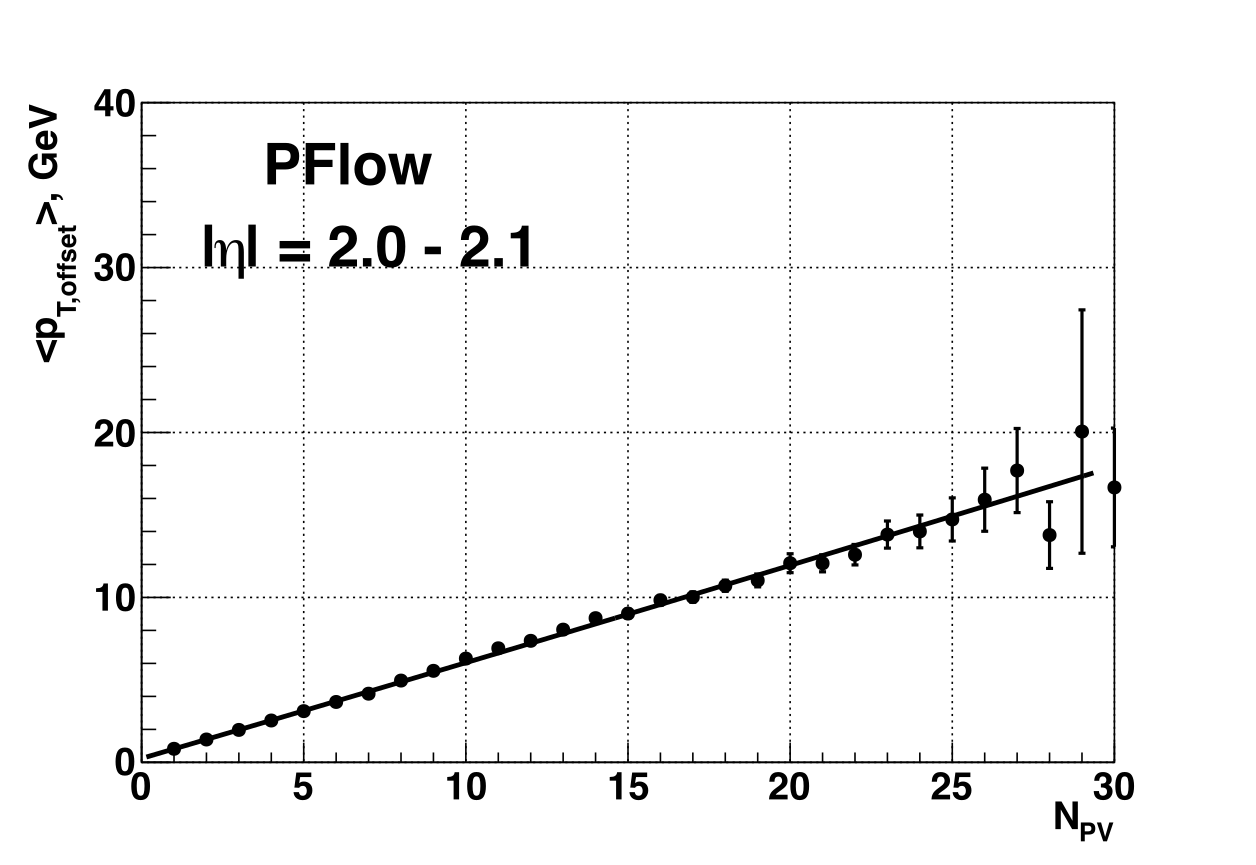
\includegraphics[width=0.45\textwidth]{chapitre4/figs/l1_offset.pdf}} \hfill
%   \subcaptionbox{\label{fig:l1_offset_vs_fastjet}}[0.45\textwidth]{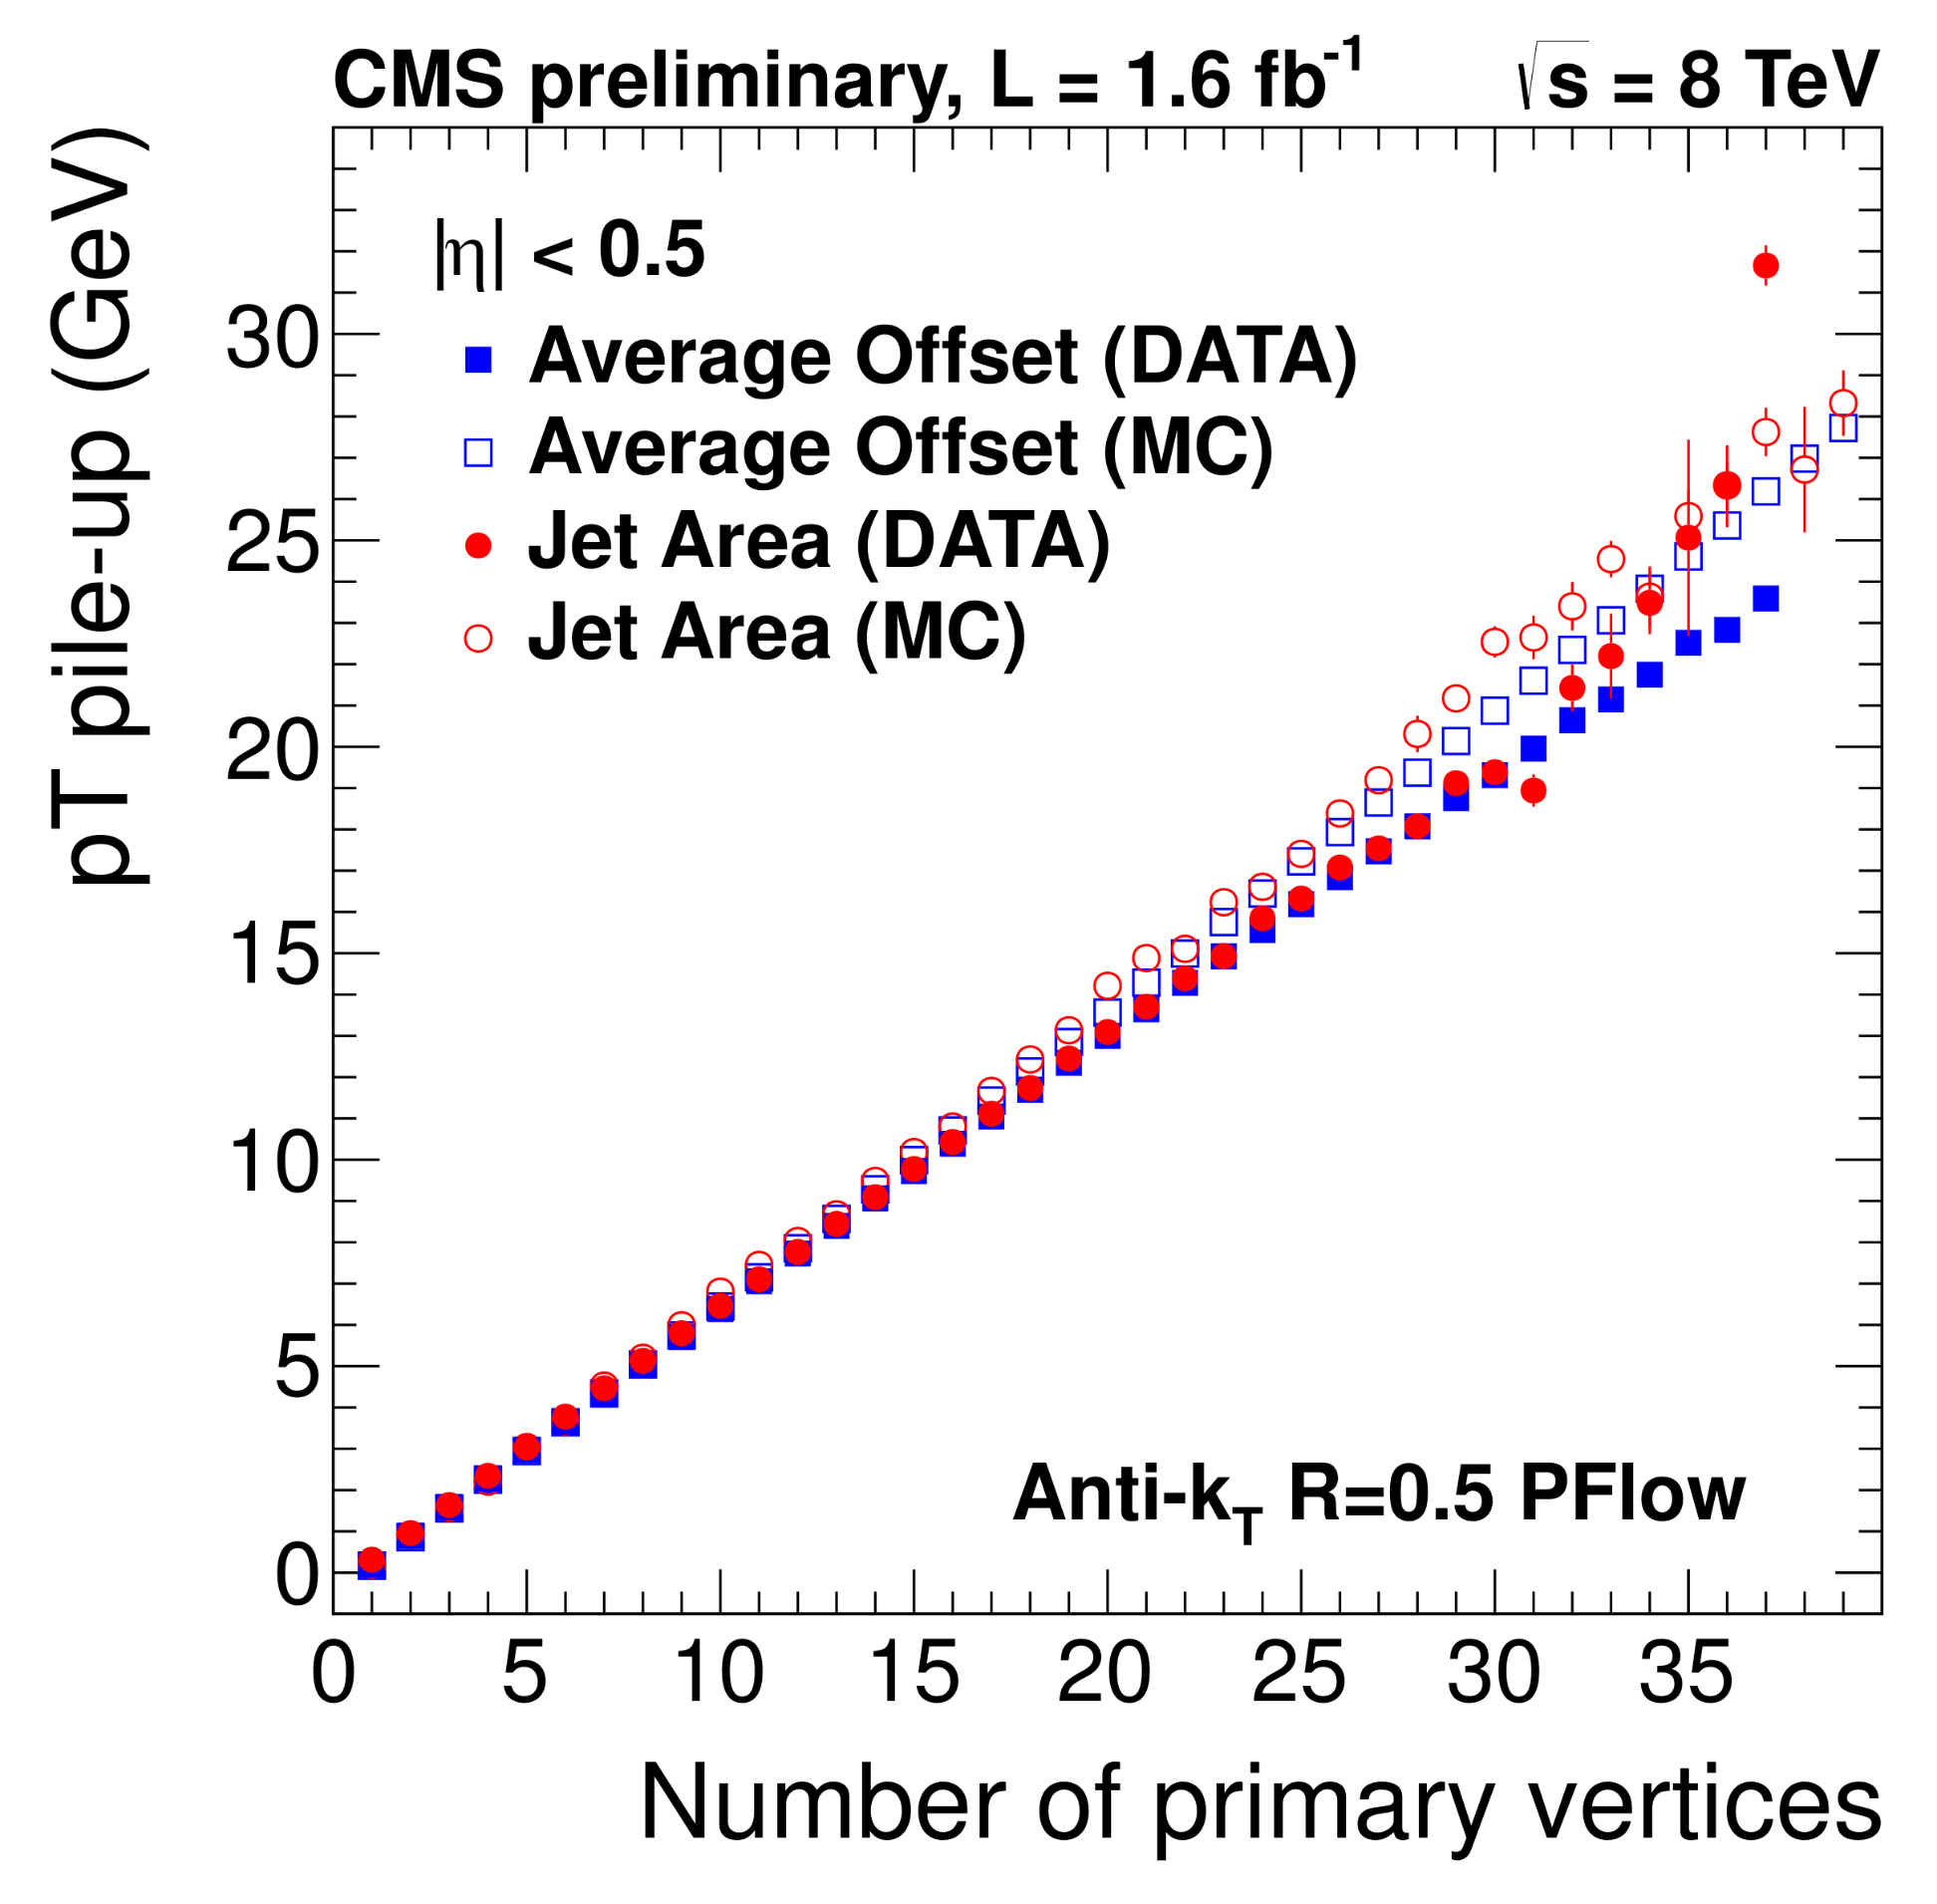
\includegraphics[width=0.45\textwidth]{chapitre4/figs/l1_offset_vs_fastjet.pdf}} \hfill
%   \caption{(\subref{fig:l1_offset}) \emph{offset} en fonction du nombre de vertex, pour $\num{2} < \aeta < \num{2.1}$, calculé sur des événements multi-jets simulés. (\subref{fig:l1_offset_vs_fastjet}) comparaison entre les méthodes \emph{offset} et \emph{fastjet}.}
%   \label{fig:jec_l1}
% \end{figure}

% \subsubsection{La méthode \emph{offset}}

% Des événements de biais minimum\footnote{Un événement de biais minimum est un événement représentatif d'une collision \Pproton{}\Pproton} sont utilisés afin d'estimer l'énergie moyenne portée par un jet à cause du \pu. \fxnote{dire pourquoi du min  bias} Cette énergie moyenne est déterminée en fonction du nombre de vertex ($N_{PV}$), ainsi qu'en fonction de $\aeta$ (voir \cref{fig:l1_offset}). On obtient ainsi une correction dépendante du nombre de vertex, ainsi que de \aeta. Cette correction est à soustraire de l'énergie du jet afin de supprimer la contribution du \pu.

% \subsubsection{La méthode \emph{fastjet}}

% Il s'avère que tous les jets ne portent pas la même énergie due au \pu. La méthode \emph{fastjet} améliore ainsi la méthode \emph{offset} en ajoutant une dépendance des corrections en fonction de l'aire des jets ($A$) et en fonction de la densité d'énergie ($\rho$), définie comme la médiane de la distribution $p_T^j / A_j$, où $j$ est l'index d'un jet dans l'événement. La correction obtenue est donc dépendante de $\rho$, de $A$ et de \aeta. On présente \cref{fig:l1_offset_vs_fastjet} une comparaison entre ces deux méthodes.

\begin{figure}
  \subcaptionbox{\label{fig:l1_no_corr}}[0.45\textwidth]{\includegraphics[width=0.45\textwidth]{chapitre4/figs/l1_effect_no_corr.pdf}} \hfill
  \subcaptionbox{\label{fig:l1_with_corr}}[0.45\textwidth]{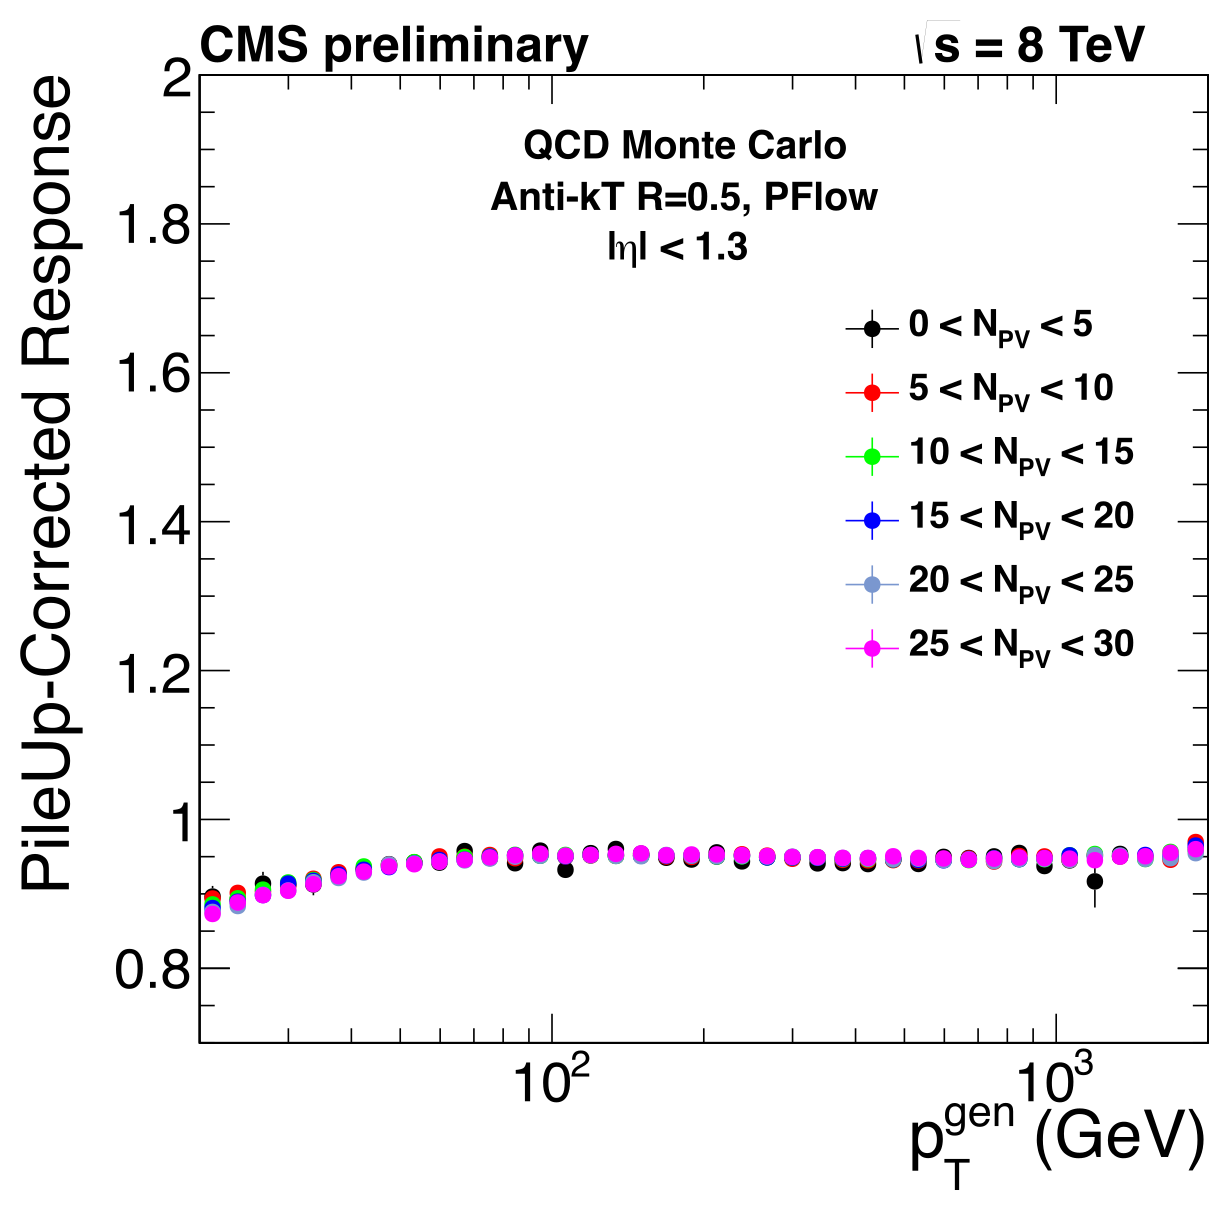
\includegraphics[width=0.45\textwidth]{chapitre4/figs/l1_effect_with_corr.pdf}} \hfill
  \caption{Évolution de la réponse des jets en fonction de l'impulsion transverse simulée, avant l'application des corrections de niveau 1 (\subref{fig:l1_no_corr}) et après (\subref{fig:l1_with_corr}), pour différentes classes de $N_{PV}$.}
  \label{fig:jec_l1_effect}
\end{figure}

\bigskip

Après application des corrections de niveau 1, la réponse des jets, définie comme le rapport en l'impulsion transverse du jet sur l'impulsion transverse vraie\footnote{L'impulsion transverse vraie d'un jet est la valeur de l'impulsion transverse dans le cas où le jet est parfaitement reconstruit. Cette valeur est déterminée en agglomérant les particules directement en sortie du générateur, plutôt que les particules après reconstruction.}, n'est plus dépendante du nombre de vertex primaires, comme on peux le voir \cref{fig:jec_l1_effect}.

\subsection[Les corrections de niveau 2 et 3]{Les corrections de niveau 2 et 3 \citep{1748-0221-6-11-P11002}} \label{sec:jec_l2l3}

Les corrections de niveau 2 (corrections en fonction de \aeta) et de niveau 3 (corrections en fonction de \pt) sont appliquées après celles de niveau 1. Ces deux niveaux de corrections forment en réalité une correction unique, la séparation en deux niveaux distincts étant purement historique.

Après les corrections de niveaux 1, la réponse n'est plus dépendante du \pu. Néanmoins, elle varie toujours en fonction de \aeta et du $p_T$. On corrige cette dépendance grâce à la simulation.

\begin{figure}[tbp]
    \centering
    \subcaptionbox{\label{fig:resp_l1l2l3}}[0.45\textwidth]{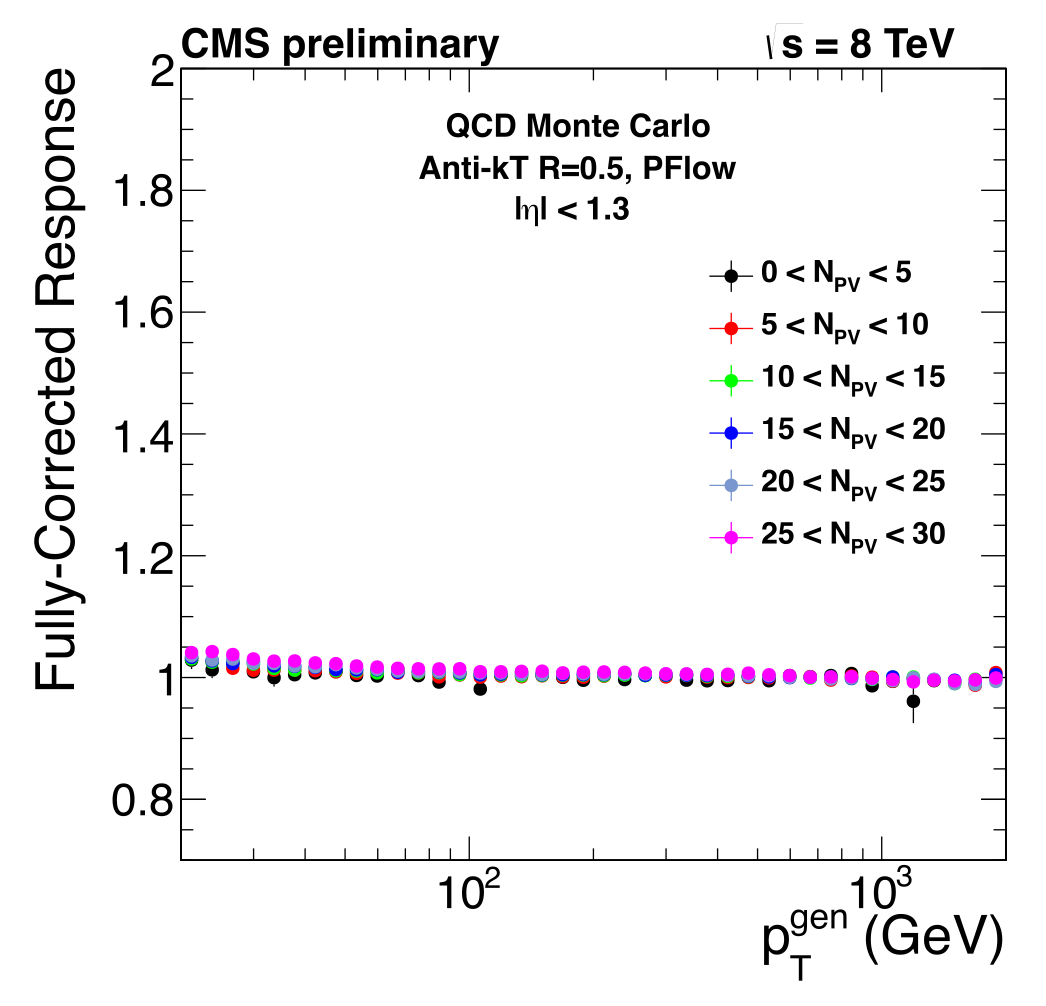
\includegraphics[width=0.45\textwidth]{chapitre4/figs/response_after_l1l2l3.pdf}} \hfill
    \subcaptionbox{\label{fig:jet_flavor_resp}}[0.45\textwidth]{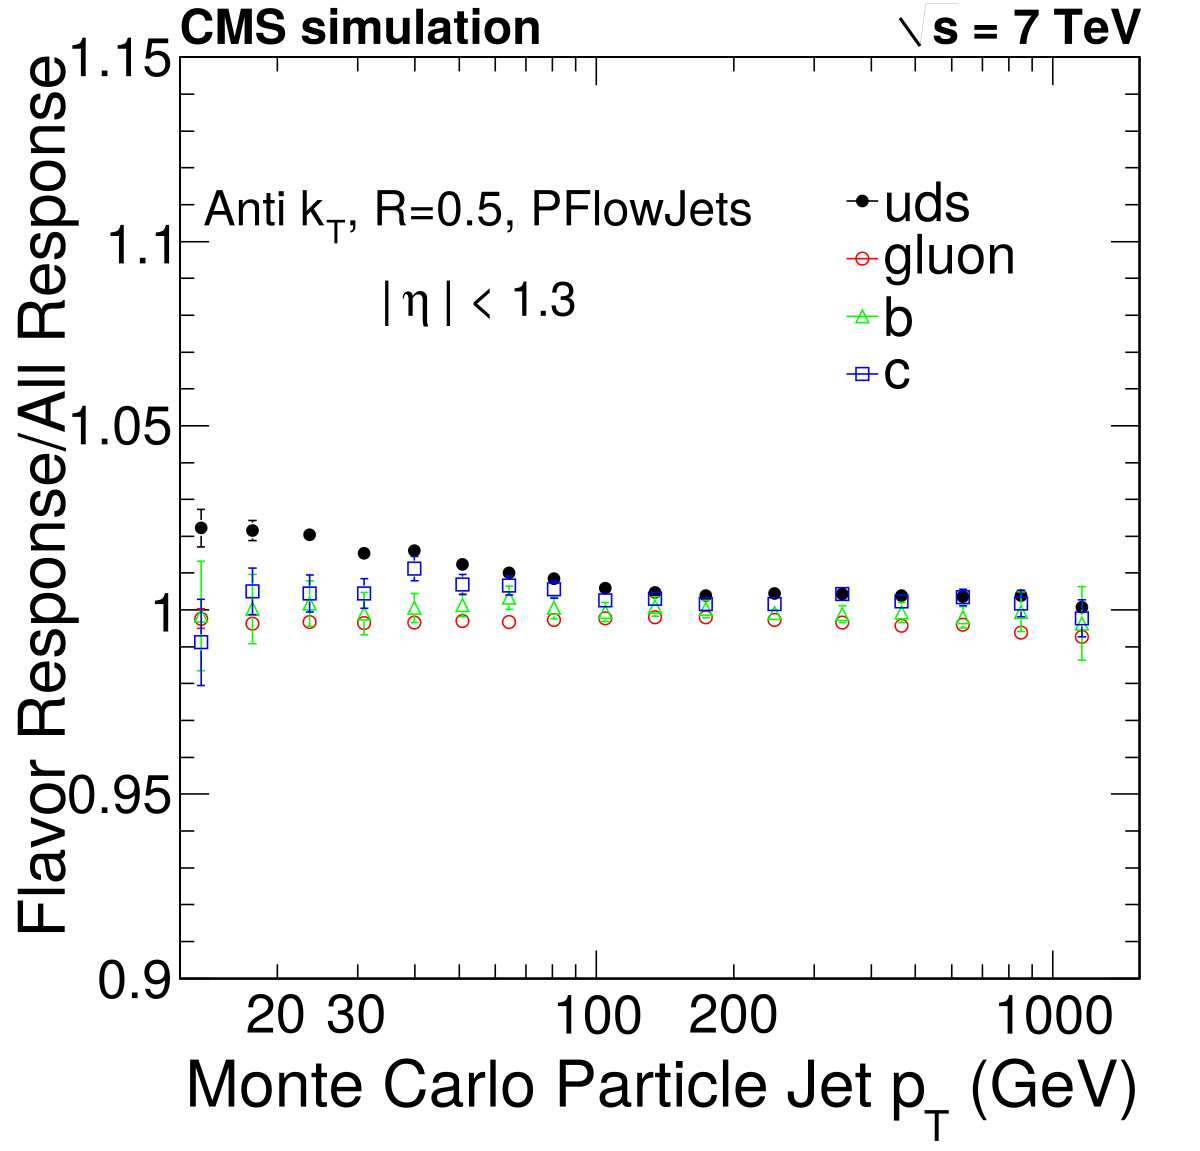
\includegraphics[width=0.45\textwidth]{chapitre4/figs/jet_flavor_response.pdf}} \hfill
    \caption{(\subref{fig:resp_l1l2l3}) Réponse des jets après application des corrections de niveau 1, 2 et 3, pour des événements multi-jets simulés. (\subref{fig:jet_flavor_resp}) Différence de réponse entre les jets légers (\Pup, \Pdown, \Pstrange), les jets de gluons, les jets de \Pcharm et les jets de \Pbottom.}
\end{figure}

\smallskip

On utilise des événements multi-jets pour déterminer les facteurs de corrections à appliquer. On réalise une grille 2D en $\eta$ et en $p_T$, et, pour chaque classe, on détermine la réponse des jets définie comme
\begin{align*}
  R &= \dfrac{p_T}{p_T^\text{vrai}}
\end{align*}
où $p_T^\text{vrai}$ est l'impulsion transverse du jet généré à partir des particules MC (impulsion transverse vraie). Le facteur de correction est alors $1 / R$, et dépend à la fois de $\eta$ et de $p_T$.


%Afin de corriger ces effets, on utilise des événements di-jets. Par conservation de l'impulsion transverse, on a donc $p_T^\text{jet 1} = p_T^\text{jet 2}$. De plus, on considère que les jets dans la région centrale du détecteur ($\aeta < \num{1.3}$) sont correctement reconstruit. On sélectionne donc des événements avec au moins un jet dans la région centrale, et on calcule la réponse $R$, définie comme $p_T^\text{jet} / p_T^\text{central}$, en fonction de \aeta et $p_T$. Dans le cas d'une reconstruction parfaite, la réponse vaut 1. Dans le cas contraire, le facteur de correction à appliquer est $1 / R$.

%\begin{figure}
  %\subcaptionbox{\label{fig:l2l3_response}}[0.45\textwidth]{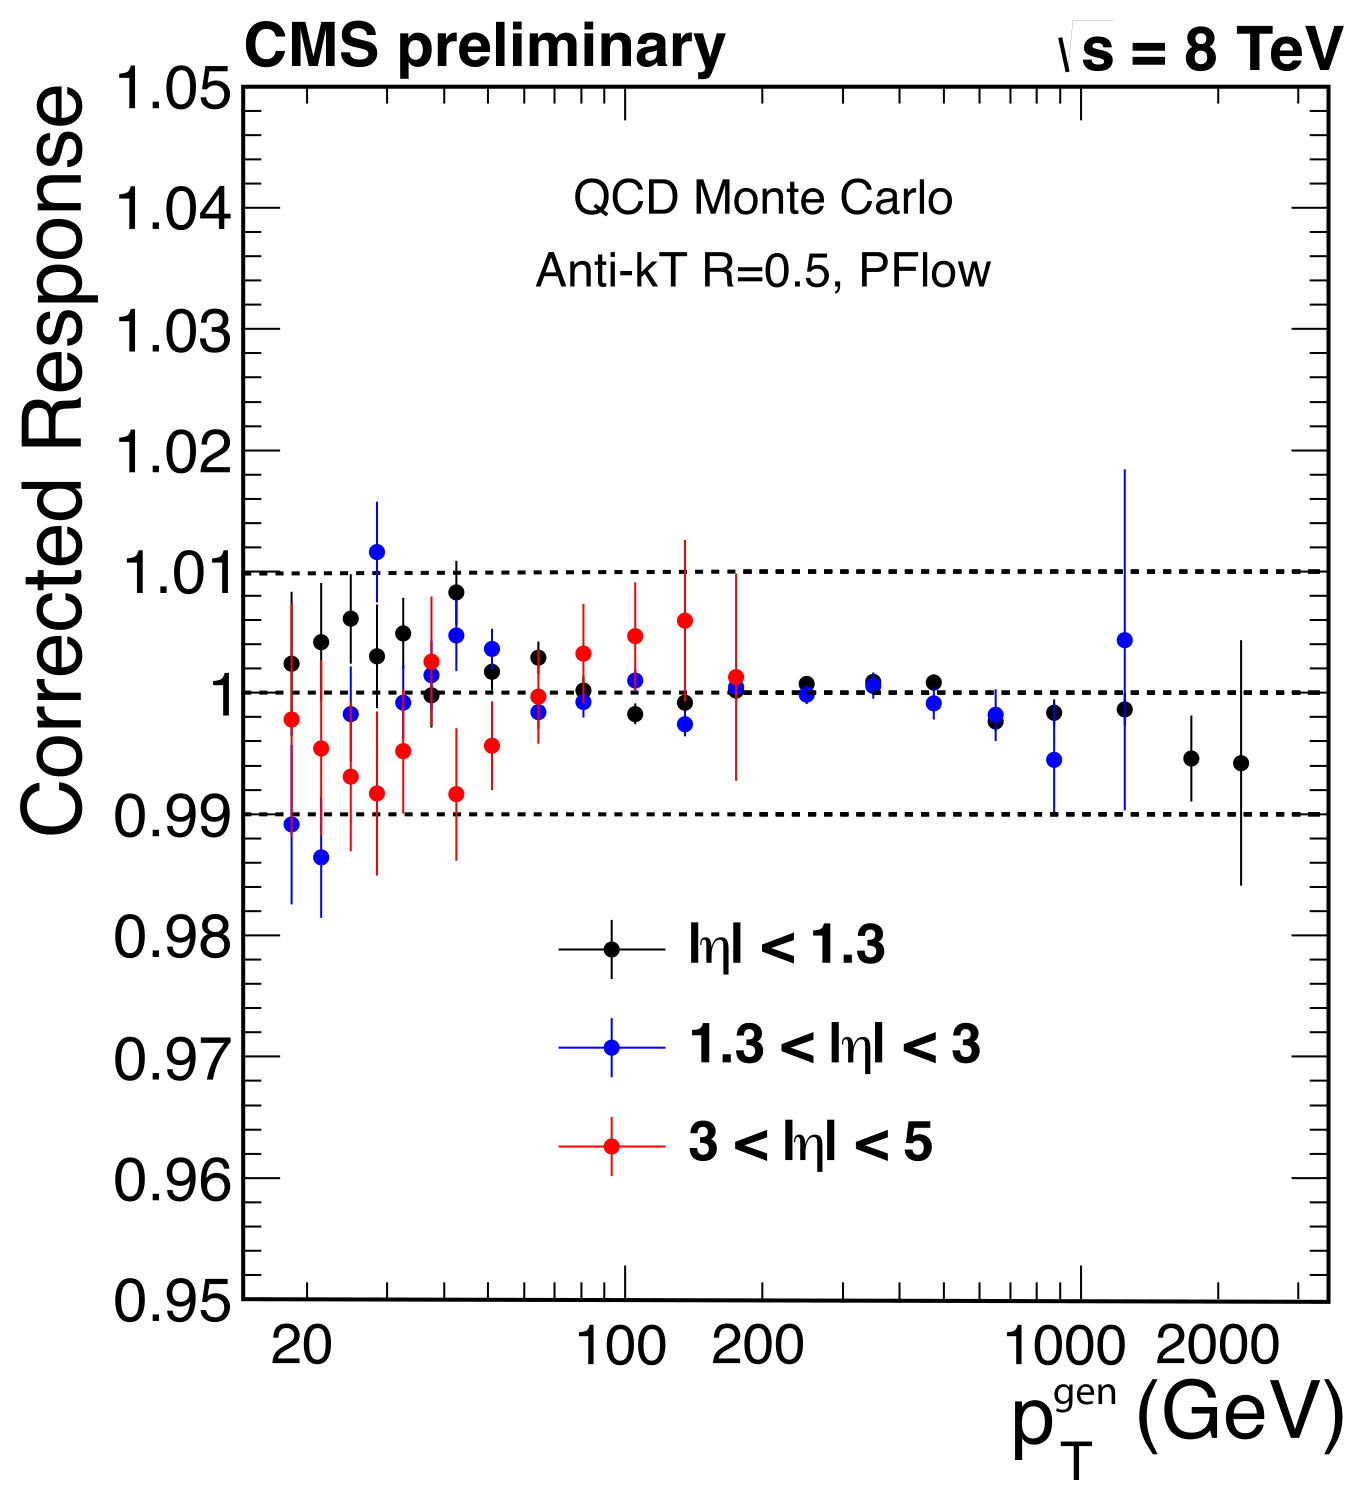
\includegraphics[width=0.45\textwidth]{chapitre4/figs/l2l3_response.pdf}} \hfill
  %\subcaptionbox{\label{fig:l1l2l3}}[0.45\textwidth]{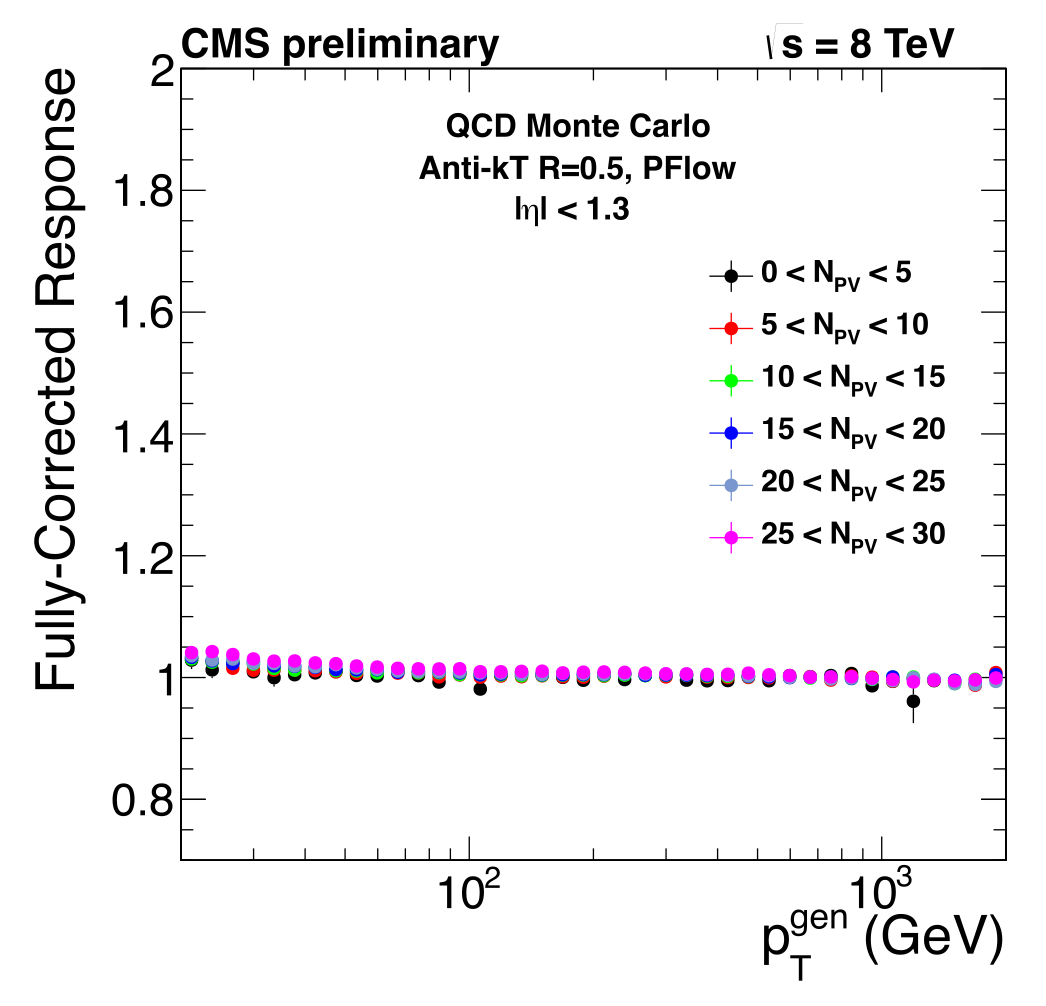
\includegraphics[width=0.45\textwidth]{chapitre4/figs/response_after_l1l2l3.pdf}} \hfill
  %\caption{Évolution de la réponse des jets en fonction de l'impulsion transverse simulée, avant l'application des corrections de niveau 1 (\subref%{fig:l1_no_corr}) et après (\subref{fig:l1_with_corr}), pour différentes classes de $N_{PV}$.}
%  \label{fig:jec_l2l3}
%\end{figure}

\bigskip

On présente \cref{fig:resp_l1l2l3} la réponse des jets après application des corrections de niveau 1, 2 et 3, pour des événements multi-jets simulés. La réponse est linéaire, c'est-à-dire indépendante de $p_T$, et vaut maintenant 1. La dépendance en $\eta$ est aussi supprimée lors de l'application des corrections de niveau 2 et 3.

\bigskip

Ces facteurs de corrections ont été déterminés sur des événements multi-jets, très riches en jets de gluons. Cependant, on peut voir \cref{fig:jet_flavor_resp} que la réponse du jet dépend de sa saveur. Pour l'instant, cette différence de réponse est prise en compte aux travers des erreurs systématiques, et on verra plus loin dans ce chapitre que des études sont menées par CMS afin de déterminer des corrections aussi dépendantes de la saveur des jets.

\subsection[Les corrections résiduelles]{Les corrections résiduelles \citep{1748-0221-6-11-P11002}} \label{sec:jec_res}

Les corrections précédentes sont toutes dérivées à l'aide de la simulation. Malheureusement, cette simulation n'est pas parfaite, et des différences existent entre la réponse des jets dans la simulation et dans les données collectées. On applique ainsi un autre niveau de corrections, uniquement sur les données, afin de corriger des dernières différences entre données et simulation. Ces corrections, dépendante de \aeta et du $p_T$ des jets, sont déterminées à l'aide d'événements $\PZ \rightarrow \left[ \Pmuon \APmuon \, | \, \Pelectron \APelectron \right] $ + jets ou $\Pphoton$ + jets, ainsi que des événements di-jets pour la dépendance en \aeta.

La détermination des corrections résiduelles à l'aide d'événement $\Pphoton$ + jets est décrite en détails dans la \cref{sec:jetmet_gamma_jet}.

\subsection{Erreurs systématiques} \label{sec:jec_uncertainties}

Face à la complexité de la détermination des corrections des jets, l'erreur systématique associée est souvent l'erreur dominante dans les analyses de physique, atteignant souvent des valeurs proches de \SI{10}{\%}. Beaucoup d'efforts sont fait pour améliorer notre compréhension des détecteurs et ainsi réduire ces erreurs systématiques.

\medskip

On trouve \cref{fig:jetmet_uncertainties} l'évolution des erreurs systématiques en fonction de \pt (\cref{fig:uncertainties_vs_pt}) et en fonction de \aeta (\cref{fig:uncertainties_vs_eta}). Cette erreur se décompose en 6 sources indépendantes :

\begin{figure}[tbp]
    \centering
    \subcaptionbox{\label{fig:uncertainties_vs_pt}}[0.45\textwidth]{\includegraphics[width=0.45\textwidth]{chapitre4/figs/uncertainties/uncertainties_vs_pt.pdf}} \qquad
    \subcaptionbox{\label{fig:uncertainties_vs_eta}}[0.45\textwidth]{\includegraphics[width=0.45\textwidth]{chapitre4/figs/uncertainties/uncertainties_vs_eta.pdf}}
    \caption{Erreurs systématiques associées aux corrections des jets en fonction de \pt (\subref{fig:uncertainties_vs_pt}) pour $\aeta \simeq 0$, et en fonction de \aeta (\subref{fig:uncertainties_vs_eta}) pour $\pt = \SI{100}{\GeV}$.}
    \label{fig:jetmet_uncertainties}
\end{figure}

\begin{itemize}
  \item Les erreurs systématiques liées à la détermination des corrections résiduelles (\emph{absolute scale} et \emph{relative scale}).
  \item Les méthodes employées pour déterminer les corrections résiduelles ne permettent pas d'aller à très bas / haut $p_T$. Une extrapolation est alors réalisée, en se basant sur les résultats obtenus à bas $p_T$. Une erreur systématique est associée à cette procédure (\emph{extrapolation}).
  \item Une erreur systématique liée à la modélisation du \pu (\pu).
  \item La différence de réponse liée à la saveur des jets est prise en compte à travers une erreur systématique dédiée (\emph{jet flavor}).
  \item Les conditions de reconstruction et de calibration du détecteur ont changé pendant la prise de données 2012. Ces différences n'ont pas été propagées à la simulation, et on voit apparaitre des différences de réponse en fonction de la date de la prise de données. Ces différences sont prises en compte \emph{via} une erreur systématique (\emph{time stability}).
\end{itemize}

On constate que la présence de \pu (ligne bleue) contribue en majorité à l'incertitude totale à bas \pt, alors que l'extrapolation devient dominante à haut \pt. De nouvelles techniques de suppression du \pu au niveau 1 sont ainsi en cours de développement, afin de réduire cette erreur systématique. Néanmoins, pour des jets de \SI{100}{\GeV} dans le tonneau ($\aeta < \num{1.3}$), l'erreur systématique totale est inférieure à \SI{2}{\%}.

\section{Détermination des corrections résiduelles à l'aide d'événements \texorpdfstring{$\Pphoton$}{γ} + jets} \label{sec:jetmet_gamma_jet}

\subsection{Intérêt des événements \texorpdfstring{$\Pphoton$}{γ} + jets}

L'application des corrections résiduelles permet de corriger des dernières différences de réponse entre la simulation et les données collectées, après calibrations de niveau 1, 2 et 3. Pour cela, on mesure la réponse des jets à la fois dans les données et dans la simulation, et on corrige les données de la différence de réponse, afin de faire en sorte que la réponse dans les données et dans la simulation soit identique. Il est donc nécessaire d'utiliser un processus physique qui permet de connaître de façon la plus précise possible l'énergie d'un jet, sans avoir à utiliser la vérité de la simulation.

\begin{figure}[t!] \centering
  \subcaptionbox{\label{fig:g_plus_jet_1}}[.4\linewidth]{
  \begin{fmfgraph*}(180,120)
    \fmfpen{0.5}
    \fmfleft{i1,i2}
    \fmfright{o1,o2}
    \fmf{gluon}{i1,v1}
    \fmf{fermion}{i2,v1}
    \fmf{fermion,label=\Pquark}{v1,v2}
    \fmf{fermion}{v2,o1}
    \fmf{photon}{v2,o2}
    \fmffreeze
    \fmfdot{v1,v2}
    \fmflabel{\Pquark}{i2}
    \fmflabel{\Pquark}{o1}
    \fmflabel{\Pphoton}{o2}
  \end{fmfgraph*}}\qquad \quad%
  % \begin{fmfgraph*}(180,120)
  %   \fmfpen{0.5}
  %   \fmfleft{i1,i2}
  %   \fmfright{o1,o2,o3}
  %   \fmf{gluon}{i2,v1}
  %   \fmf{gluon}{v3,o1}
  %   \fmf{fermion}{i1,v3}
  %   \fmf{fermion,label=\APquark}{v3,v2,v1}
  %   \fmf{fermion}{v1,o3}
  %   \fmffreeze
  %   \fmf{photon,label=\Pphoton}{v2,o2}
  %   \fmfdot{v1,v2,v3}
  %   \fmflabel{\Pquark}{i1}
  %   \fmflabel{\Pquark}{o3}
  % \end{fmfgraph*}}\qquad \quad%
  \subcaptionbox{\label{fig:g_plus_jet_2}}[.4\linewidth]{
  % \begin{fmfgraph*}(180,120)
  %   \fmfpen{0.5}
  %   \fmfstraight
  %   \fmfleft{i1,i2}
  %   \fmfright{o1,o2,o3}
  %   \fmf{fermion}{i1,v1,i2}
  %   \fmf{fermion}{v4,v2}
  %   \fmf{phantom}{o1,v4}
  %   \fmf{fermion,label=\Pquark}{v2,v3}
  %   \fmf{photon,label=$\Pphoton$}{v3,o3}
  %   \fmf{gluon}{v1,v2}
  %   \fmffreeze
  %   \fmf{fermion}{v3,o2}
  %   \fmfdot{v1,v2,v3}
  %   \fmflabel{\APquark}{i2}
  %   \fmflabel{\Pquark}{i1}
  %   \fmflabel{\Pquark}{o2}
  %   \fmflabel{\APquark}{v4}
  % \end{fmfgraph*}
  \begin{fmfgraph*}(180,120)
    \fmfpen{0.5}
    \fmfstraight
    \fmfleft{i1,i2}
    \fmfright{o1,o2,o3}
    \fmf{fermion}{i2,v3}
    \fmf{fermion,label=\APquark}{v3,v2}
    \fmf{gluon}{i1,v1,o1}
    \fmf{gluon}{v2,v1}
    \fmf{photon}{v3,o3}
    \fmffreeze
    \fmf{fermion}{v2,o2}
    \fmflabel{\Pquark}{i2}
    \fmflabel{\Pquark}{o2}
    \fmflabel{\Pphoton}{o3}
  \end{fmfgraph*}
  }
  \caption{Exemples de diagrammes de Feynman associés à la production d'un photon et d'un jet (\subref{fig:g_plus_jet_1}) et d'un photon et de deux jets (\subref{fig:g_plus_jet_2}).}
  \label{fig:gamma_jet_diagrams}
\end{figure}

On utilise pour cela des processus comportant uniquement deux particules dans l'état final : une particule dont on connaît très bien les propriétés (boson \PZ, photon, \ldots), qui sera notre sonde, et un jet. On utilise ensuite les propriétés de la sonde pour déterminer celles du jet. Par la suite, seuls les événements \Pphoton + jets seront abordés.

\bigskip

On présente \cref{fig:gamma_jet_diagrams} deux diagrammes de Feynman représentant la production d'un photon accompagné d'un ou deux jets. L'impulsion dans le plan transverse étant nulle au moment de la collision, on a dans l'état final
\begin{align*}
  \vec{p}_T &= 0 = \vec{p}_{T}^{\Pphoton} + \vec{p}_T^\text{jet}\\
  \norm{\vec{p}_T^{\Pphoton}} &= \norm{\vec{p}_T^{\text{jet}}}
\end{align*}

Ainsi, il est suffisant de connaître l'impulsion transverse de la sonde pour déterminer l'impulsion transverse du jet. L'utilisation du photon comme sonde comporte certains avantages :
\begin{itemize}
  \item Comme on a déjà pu le voir lors du \cref{chap:reco}, le calorimètre électromagnétique est bien plus performant que le calorimètre hadronique. La résolution sur la reconstruction des photons est \tilde\SI{2}{\%}, contre \tilde{10}{\%} pour les jets.
  \item Comparé à d'autres processus comme \PZ + jets, la section efficace de production \Pphoton + jets au LHC à \SI{8}{\TeV} est bien plus grande : le nombre d'événements disponible est ainsi plus important.
  \item La production d'événements \Pphoton + jets n'est pas résonante, à la différence des événements \PZ + jets. Il est ainsi possible d'explorer une gamme en impulsion transverse beaucoup plus large.
\end{itemize}

\subsection{Détermination de la réponse des jets}

% On cherche à déterminer la réponse $R$ des jets, qui tend vers 1 si l'on reconstruit parfaitement le jet. On utilise deux méthodes différentes pour déterminer cette réponse : la méthode de la balance et la méthode MPF, détaillées ci-dessous.

Deux méthodes différentes sont utilisées afin de déterminer la réponse $R$ des jets : la méthode de la balance et la méthode MPF, détaillées ci-dessous.

\subsubsection{La méthode de la balance}

On utilise le principe de conservation de l'impulsion transverse. Pour un événement où le photon est parfaitement équilibré avec le jet dans le plan transverse, on a
\begin{align*}
  \norm{\vec{p}_T^{\Pphoton}} &= \norm{\vec{p}_T^{jet}}
\end{align*}
et on défini la réponse $R$ par la relation
\begin{align*}
    R &= \frac{p_T^\text{jet}}{p_T^{\Pphoton}}
\end{align*}

Cette méthode est très simple et performante. Néanmoins, elle est très sensible au \pu, ainsi qu'aux radiations dans l'état final. En effet, la présence d'autres jets dans l'état final vont venir perturber la balance entre le jet et le photon. Il est cependant possible de restaurer cet équilibre, en utilisant une extrapolation.

\paragraph{L'extrapolation}

La balance entre le photon et le jet est perturbée par la présence de jets additionnels dans l'événement, provenant de radiations dans l'état final. On définit $\alpha$ comme le rapport entre l'impulsion transverse du second jet de l'événement et l'impulsion transverse du photon,
\begin{align*}
    \alpha &= \frac{p_T^{\text{\ordinalnum{2} jet}}}{p_T^\gamma}
\end{align*}

Afin de réduire l'influence des jets additionnels sur la réponse, on effectue un découpage de la réponse en $\alpha$, et on extrapole le comportement de la réponse pour $\alpha \rightarrow 0$.

\subsubsection{La méthode MPF (\emph{Missing $E_T$ projection fraction})} \label{sec:mpf}

Un événement \Pphoton + jets n'a pas d'énergie transverse manquante. Ainsi, au niveau partonique, on a
\begin{align*}
  \vec{p}_T^{\Pphoton} + \vec{p}_T^{\text{recul}} &= -\vec{\met} = \vec{0}
\end{align*}
où $\vec{p}_T^{\text{recul}}$ est le vecteur impulsion transverse de toutes les particules dans l'événement différentes du photon.

Après reconstruction, on a
\begin{align*}
  R_{\Pphoton} \, \vec{p}_T^{\Pphoton} + R_{\text{recul}} \, \vec{p}_T^{\text{recul}} &= -\vec{\met}
\end{align*}
$R_X$ désigne ici la réponse des détecteurs lors de la reconstruction de l'objet $X$.

On considère que les photons sont reconstruits de façon parfaite, on pose donc $R_{\Pphoton} = 1$. En utilisant le fait que $\vec{p}_T^{\text{recul}} = -\vec{p}_T^{\Pphoton}$ on obtient
\begin{align*}
  R_{\text{recul}} &= 1 + \frac{\vec{\met} \cdot \vec{p}_T^{\Pphoton}}{\left( p_T^{\Pphoton} \right)^2} \equiv R_{\text{MPF}}
\end{align*}

À la différence de la méthode de la balance, cette méthode n'est pas dépendante de la présence de jets additionnels dans l'événement, mais requiert par contre une excellente reconstruction de l'énergie transverse manquante. C'est le cas dans CMS grâce à l'utilisation de l'algorithme du \pf.

\medskip

Cette méthode est utilisée pour produire les corrections officielles. La méthode de la balance permet de vérifier la compatibilité des corrections obtenues.

\end{fmffile}

\subsection{Sélection des événements} \label{sec:jetmet_sel}

Pour déterminer les corrections résiduelles, on sélectionne sur les données des événements contenant un unique photon, ainsi qu'un ou deux jets. Le principal bruit de fond est dû aux événements multi-jets où un jet est incorrectement identifié comme un photon. On étudie les performances de notre sélection sur des événement \Pphoton + jets simulés, considérés comme notre signal, ainsi que sur des événements multi-jets, le bruit de fond.

Afin d'éliminer une grande partie du bruit de fond, une sélection est appliquée. La première étape consiste à sélectionner des événements contenant uniquement un seul photon. On utilise pour cela une méthode d'identification des photons. Suivant les besoin des analyses, cette méthode peut être optimisée pour obtenir une grande efficacité de sélection et une faible pureté (beaucoup d'événements sont sélectionnés, mais certains ne sont pas des vrais photons) ou au contraire une grande pureté et une faible efficacité (moins d'événements sont sélectionnés, mais la probabilité qu'ils ne soient pas de vrais photons est très faible).

On souhaite obtenir les événements les plus purs possible. On choisit donc le point de fonctionnement offrant la plus grande pureté (\tilde\SI{96}{\%} des photons sont des vrais photons), mais une efficacité plus faible ($\tilde \SI{70}{\%}$). Cette identification est définie de la façon suivante :

\begin{enumerate}
    \item Un contrôle est effectué pour vérifier que le photon n'est pas en réalité un électron dont la trace n'a pas pu être liée au dépôt calorimétrique, et qu'il ne provient pas du rayonnement bremsstrahlung d'un électron lors de son passage dans le ECAL.
    \item Le ratio entre l'énergie collectée dans le calorimètre hadronique et l'énergie collectée dans le calorimètre électromagnétique doit être inférieur à \SI{5}{\%}. La majorité de l'énergie doit donc être déposée dans le calorimètre électromagnétique.
    \item $\sigma_{i\eta i\eta} < \num{0.011}$. Cette variable représente la largeur de l'agrégat calorimétrique en \aeta, et est caractéristique de la forme de la gerbe électronique dans le calorimètre électromagnétique, plus étalée dans le cas d'un électron que d'un photon.
\end{enumerate}

En plus de ces trois critères, on demande que le photon soit isolé. On définit l'isolation $I$ comme le rapport entre l'énergie de toutes les particules \pf contenues dans un cône de rayon $\Delta R = \num{0.3}$ centré autour du photon et l'énergie du photon. Cette valeur étant hautement sensible au \pu, on applique une procédure qui permet de diminuer son impact, en corrigeant cette isolation par un facteur dépendant de la densité d'énergie $\rho$. On a ainsi $I_\text{corr} = \max{\left(I - f(\rho), 0\right)}$. On effectue des coupures sur cette isolation selon trois différents types de particules : les hadrons neutres, chargés, et les photons :

\begin{itemize}
    \item $I_\text{hadrons neutres} < \num{0.4} + \num{0.04} \, p_T^{\Pphoton}$
    \item $I_\text{hadrons chargés} < \num{0.7}$
    \item $I_\text{photons} < \num{0.5} + \num{0.005} \, p_T^{\Pphoton}$
\end{itemize}

Afin de ne garder que les photons les mieux reconstruits, on sélectionne uniquement ceux reconstruits dans le tonneau, avec $\aeta < \num{1.3}$, et une impulsion transverse d'au moins \SI{40}{\GeV}.

\medskip

\begin{figure}[tbp] \centering
  \subcaptionbox{\label{fig:schema_gamma_jet}}[0.45\textwidth]{\scalebox{2}{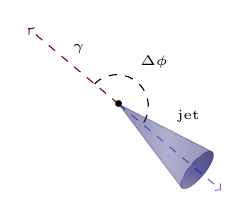
\begin{tikzpicture}[rotate=45]
    \draw[draw=red!50!black,dashed,->] (0:0) -- (95:1.5) ;
    \draw (90:1) node[right] {\tiny $\gamma$} ;

    \draw[draw=blue!60,dashed,->] (0:0) -- (-85:1.7) ;

    \draw[dashed] (95:4mm) arc (90:-80:4mm) ;
    \draw (5:7mm) node {\tiny $\Delta\phi$} ;

    \begin{scope}[rotate=5]
      \fill[top color=blue!50!black,bottom color=blue!10,middle color=blue,shading=axis,opacity=0.25] (0,-13mm) circle (3mm and 1mm);
      \fill[left color=blue!50!black,right color=blue!50!black,middle color=blue!50,shading=axis,opacity=0.25] (3mm,-13mm) -- (0,0mm) -- (-3mm,-13mm) arc (180:360:3mm and 1mm);
      \draw[draw=blue!50!black,opacity=0.25] (-3mm,-13mm) arc (180:360:3mm and 1mm) -- (0,0mm) -- cycle;
      \draw[draw=blue!50!black,opacity=0.25,densely dashed] (-3mm,-13mm) arc (180:0:3mm and 1mm);
    \end{scope}

    \draw (-55:0.9) node {\tiny jet} ;
    \draw (0:0) node {\tiny $\bullet$} ;

  \end{tikzpicture}}} \quad
  \subcaptionbox{\label{fig:schema_gamma_jets}}[0.45\textwidth]{\scalebox{2}{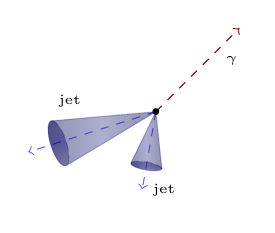
\begin{tikzpicture}
    \draw[draw=red!50!black,dashed,->] (0:0) -- (45:1.5) ;
    \draw (40:1) node[right] {\tiny $\gamma$} ;

    \draw[draw=blue!60,dashed,->] (0:0) -- (-100:1) ;
    \draw[draw=blue!60,dashed,->] (0:0) -- (-162.5:1.7) ;

    \begin{scope}[rotate=-72]
      \fill[top color=blue!50!black,bottom color=blue!10,middle color=blue,shading=axis,opacity=0.25] (0,-13mm) circle (3mm and 1mm);
      \fill[left color=blue!50!black,right color=blue!50!black,middle color=blue!50,shading=axis,opacity=0.25] (3mm,-13mm) -- (0,0mm) -- (-3mm,-13mm) arc (180:360:3mm and 1mm);
      \draw[draw=blue!50!black,opacity=0.25] (-3mm,-13mm) arc (180:360:3mm and 1mm) -- (0,0mm) -- cycle;
      \draw[draw=blue!50!black,opacity=0.25,densely dashed] (-3mm,-13mm) arc (180:0:3mm and 1mm);
    \end{scope}

    \begin{scope}[rotate=-10]
      \fill[top color=blue!50!black,bottom color=blue!10,middle color=blue,shading=axis,opacity=0.25] (0,-7mm) circle (2mm and 0.5mm);
      \fill[left color=blue!50!black,right color=blue!50!black,middle color=blue!50,shading=axis,opacity=0.25] (2mm,-7mm) -- (0,0mm) -- (-2mm,-7mm) arc (180:360:2mm and 0.5mm);
      \draw[draw=blue!50!black,opacity=0.25] (-2mm,-7mm) arc (180:360:2mm and 0.5mm) -- (0,0mm) -- cycle;
      \draw[draw=blue!50!black,opacity=0.25,densely dashed] (-2mm,-7mm) arc (180:0:2mm and 0.5mm);
    \end{scope}

    \draw (-84:1) node {\tiny jet} ;
    \draw (-187:1.1) node {\tiny jet} ;
    \draw (0:0) node {\tiny $\bullet$} ;

  \end{tikzpicture}}}
  \caption{Un événement $\gamma$ + jets parfaitement dos-à-dos (\subref{fig:schema_gamma_jet}) et où la balance est brisée (\subref{fig:schema_gamma_jets}).}
  \label{fig:schema_g_jet}
\end{figure}

On demande au moins un jet dans l'événement, reconstruit grâce à l'algorithme anti-$k_T$, avec une largeur de cône $R = \num{0.5}$, composé d'au moins deux particules. Cette identification est très efficace ($> \SI{99}{\%}$) et permet d'éliminer les faux jets dû à des bruits dans les détecteurs. La séparation azimutale $\abs{\Delta \phi}$ dans le plan transverse entre le photon et le premier jet de l'événement doit être supérieure à \SI{2.8}{\radian}, afin de ne conserver que les événements où le photon et le jet sont dos-à-dos. Les \cref{fig:schema_gamma_jet,fig:schema_gamma_jets} représentent un événement $\Pphoton$ + jets avec 1 ou 2 jets. Dans le cas où un second jet est présent, on vérifie que son énergie est inférieure à \SI{20}{\%} de celle du photon ($\alpha < \num{0.20}$), afin d'éviter de conserver des événements trop déséquilibrés. Cette condition n'est appliquée que si $p_T^{\text{\ordinalnum{2} jet}} \geq \SI{10}{\GeV}$. Tous les jets sont corrigés avec les corrections de niveau 1, 2 et 3.

\label{page:met_propagation} Toutes les corrections effectuées sur les jets sont ensuite propagées à l'énergie transverse manquante. En effet, on rappelle que \met est définie comme l'opposé de la somme vectorielle des impulsions transverses de toutes les particules de l'événement. Si jamais l'impulsion d'une particule est modifiée après calcul de \met, il est nécessaire de propager ces modifications afin de garder une définition cohérente de l'énergie transverse manquante. Ainsi, si pour un jet, on procède à la correction suivante :
\begin{align*}
  p_x \rightarrow p_x + \Delta p_x \\
  p_y \rightarrow p_y + \Delta p_y
\end{align*}
la correction à appliquer sur l'énergie transverse manquante est :
\begin{align*}
  \METx^{\text{corr}} &= \METx - \Delta p_x \\
  \METy^{\text{corr}} &= \METy - \Delta p_y
\end{align*}

Pour terminer la sélection, un véto est imposé sur la présence d'électrons ou de muons isolés dans l'événement. Sur des événements de signal simulés, cette sélection a une efficacité de \tilde \SI{20}{\%}, et inférieure à \tilde\SI{1}{‰} sur le bruit de fond.

\bigskip

Sur les données, on demande à ce que les événements aient passé les chemins de déclenchement demandant un photon isolé. Plusieurs de ces chemins existent en fonction de l'impulsion du photon, dont la plupart avec un facteur de \emph{prescale}\footnote{Il arrive que certains chemins de déclenchement laissent passer trop d'événements. Afin d'éviter de surcharger le HLT, on applique un facteur de \emph{prescale}, définit comme l'inverse de la probabilité de garder un événement. Plus ce facteur est grand, moins les événements ont de chance d'être conservés.} différent de 1. Afin de pouvoir comparer les données et la simulation sans être gêné par ce facteur, on applique une coupure supplémentaire sur l'impulsion transverse du photon à \SI{175}{\GeV}. Cette coupure n'est pas appliquée pour déterminer les facteurs de corrections, mais uniquement pour comparer les distributions.

\smallskip

Finalement, la simulation des événements multi-jets et $\gamma$ + jets a été effectuée pendant la prise de données. À cette époque, le profil de \pu n'était pas encore connu précisément, et une estimation de ce profil a été utilisée pour la simulation. On repondère donc le profil de \pu de la simulation pour qu'il corresponde à celui observé sur les données collectées.

\begin{figure}[p]
    \centering
    \subcaptionbox{\label{pt_photon}}[0.45\textwidth]{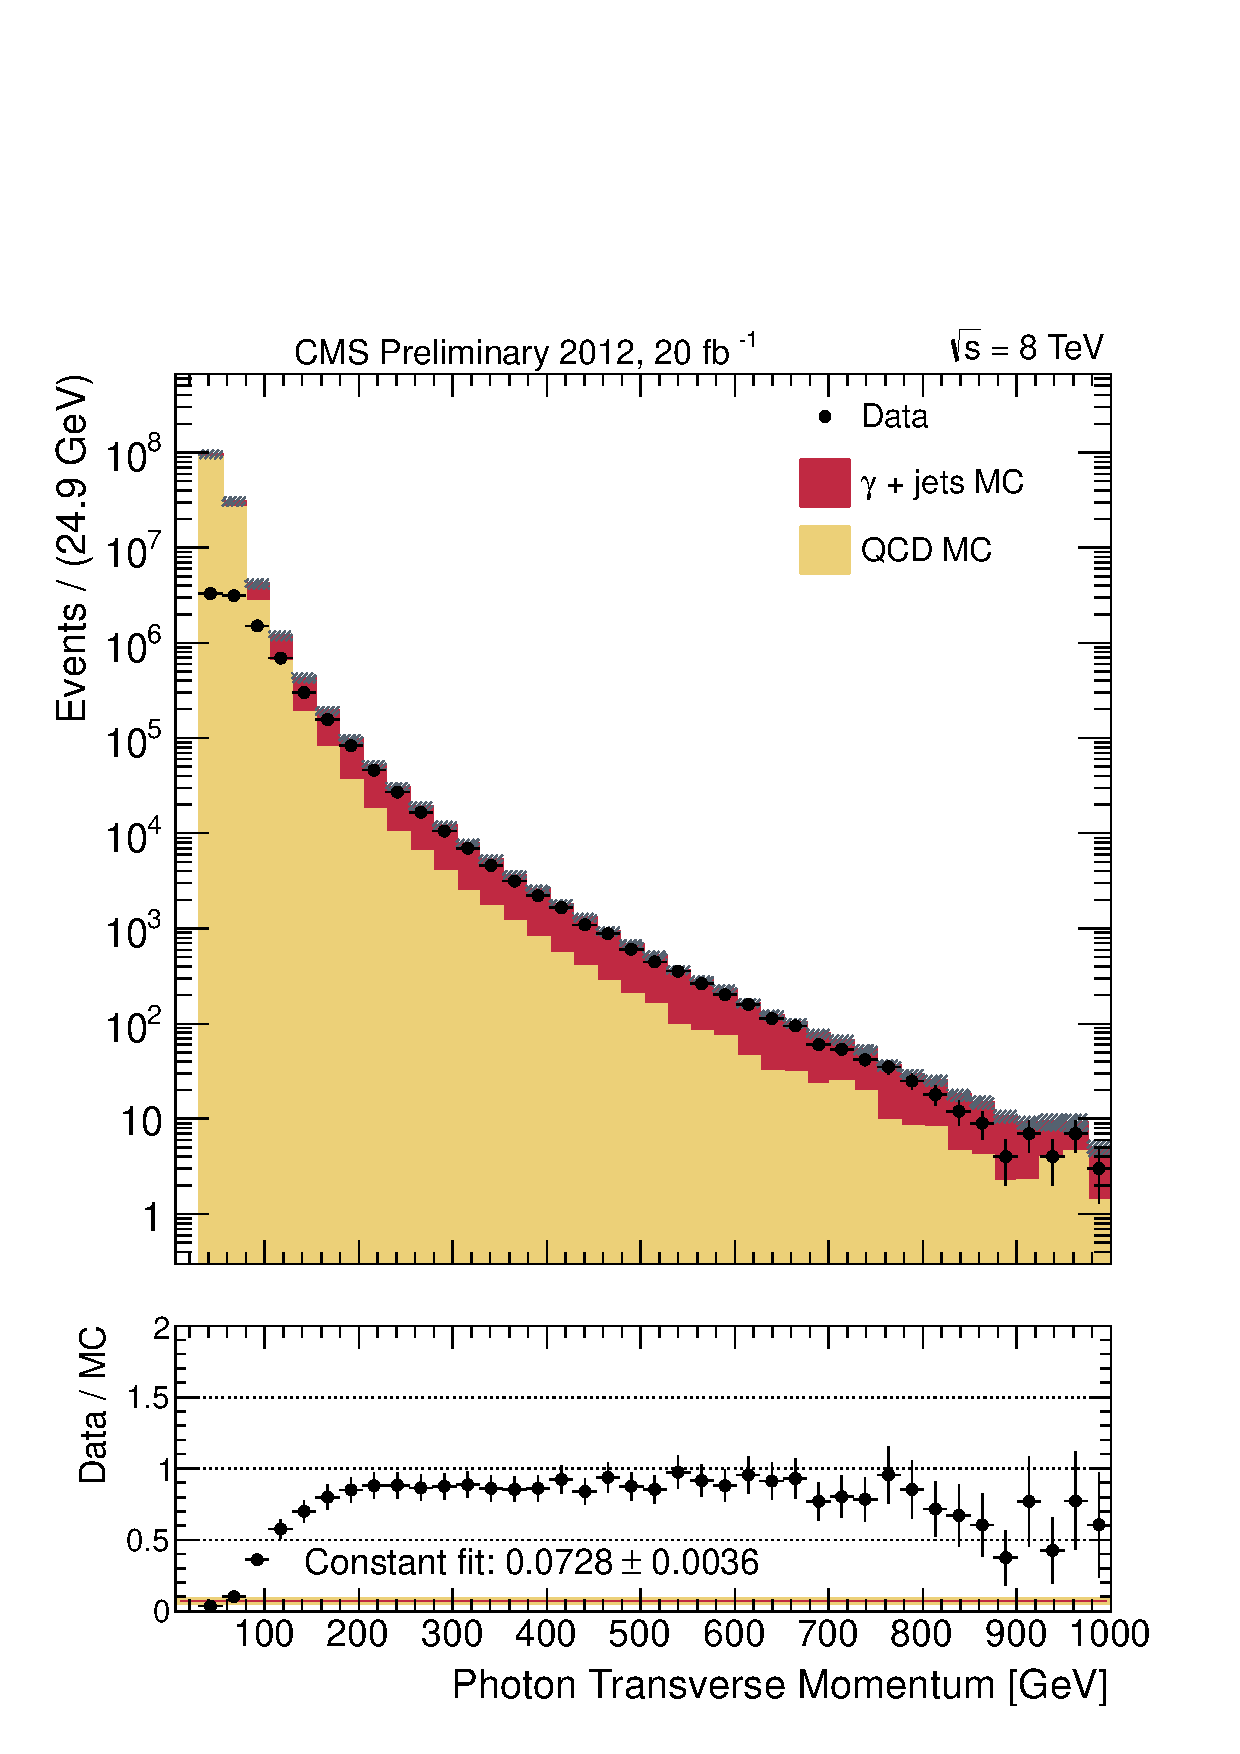
\includegraphics[width=0.45\textwidth]{chapitre4/figs/ptPhoton_passedID_log.pdf}}\hfill
    \subcaptionbox{\label{pt_first_jet}}[0.45\textwidth]{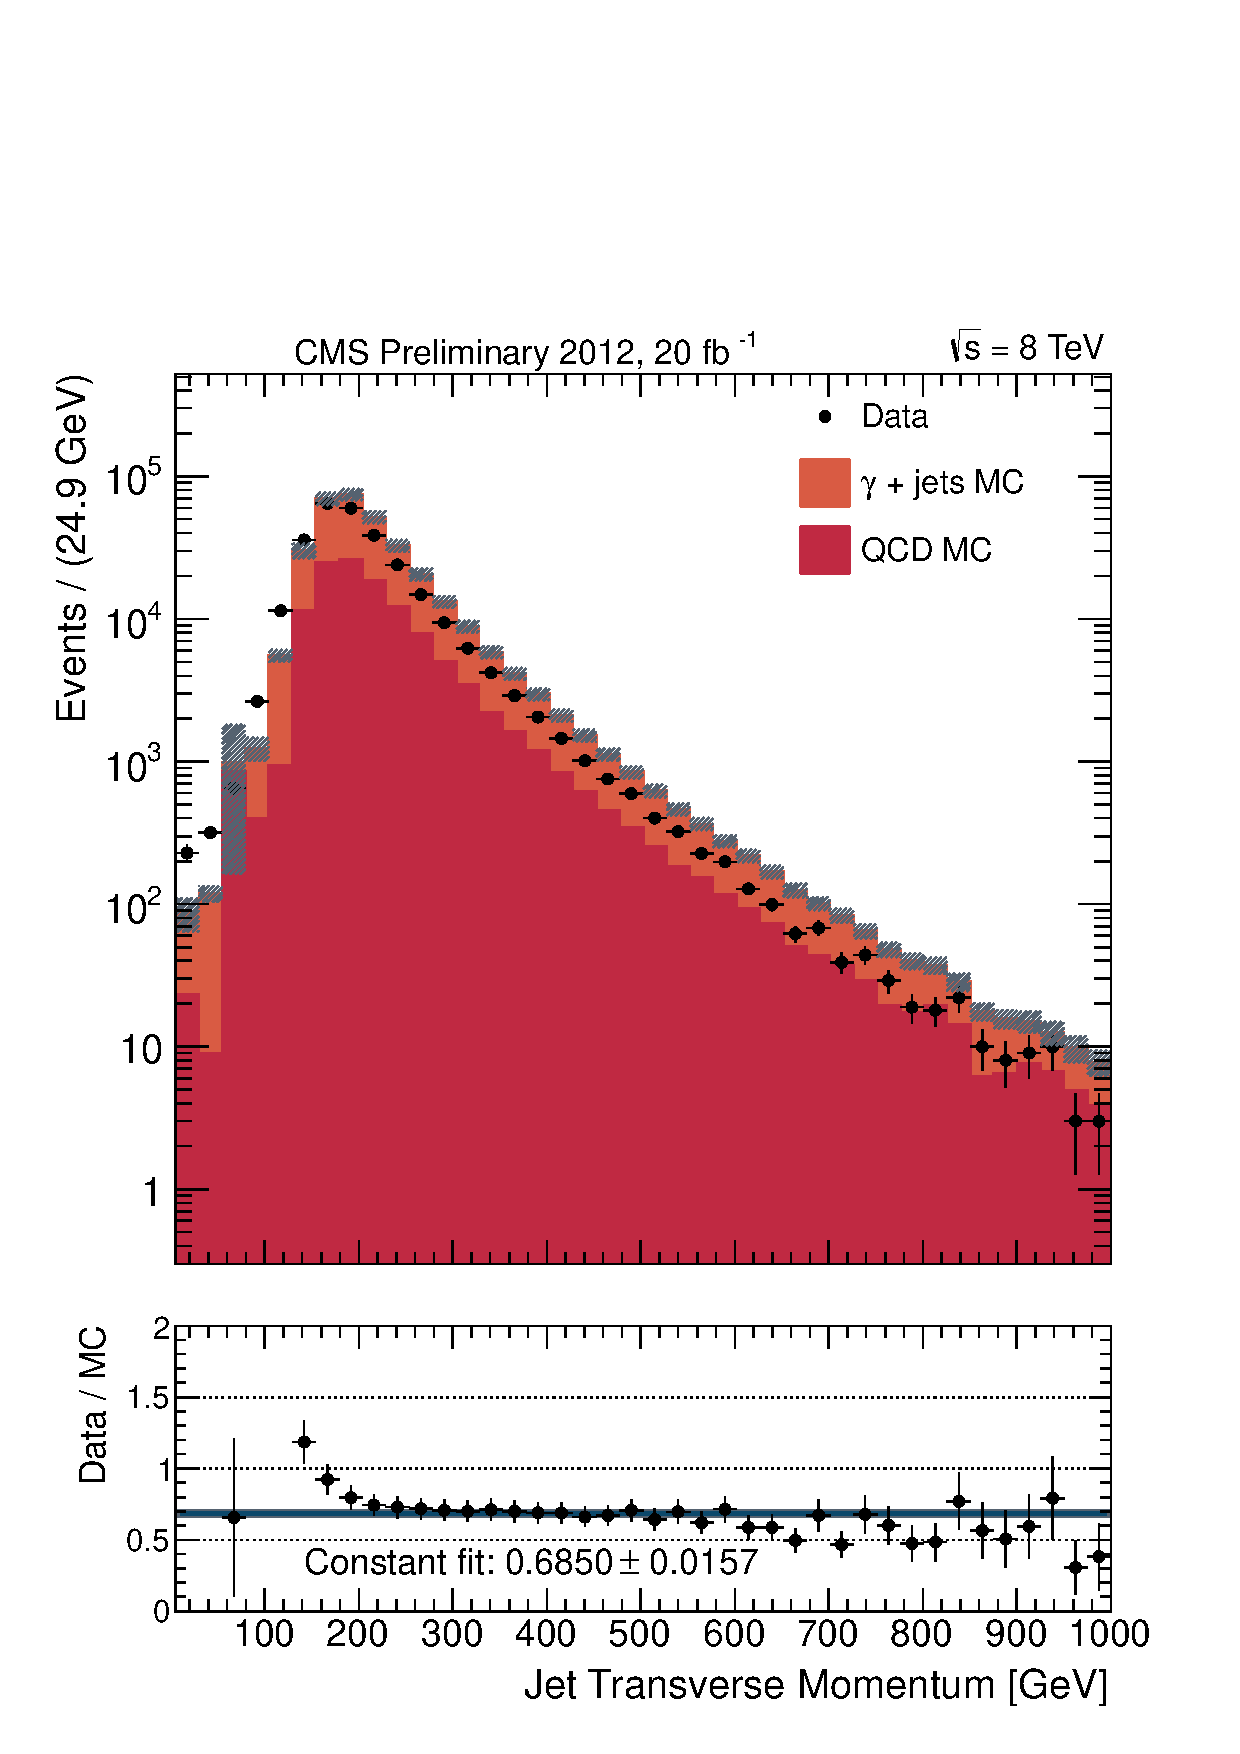
\includegraphics[width=0.45\textwidth]{chapitre4/figs/ptFirstJet_passedID_log.pdf}}
    \subcaptionbox{\label{pt_second_jet}}[0.45\textwidth]{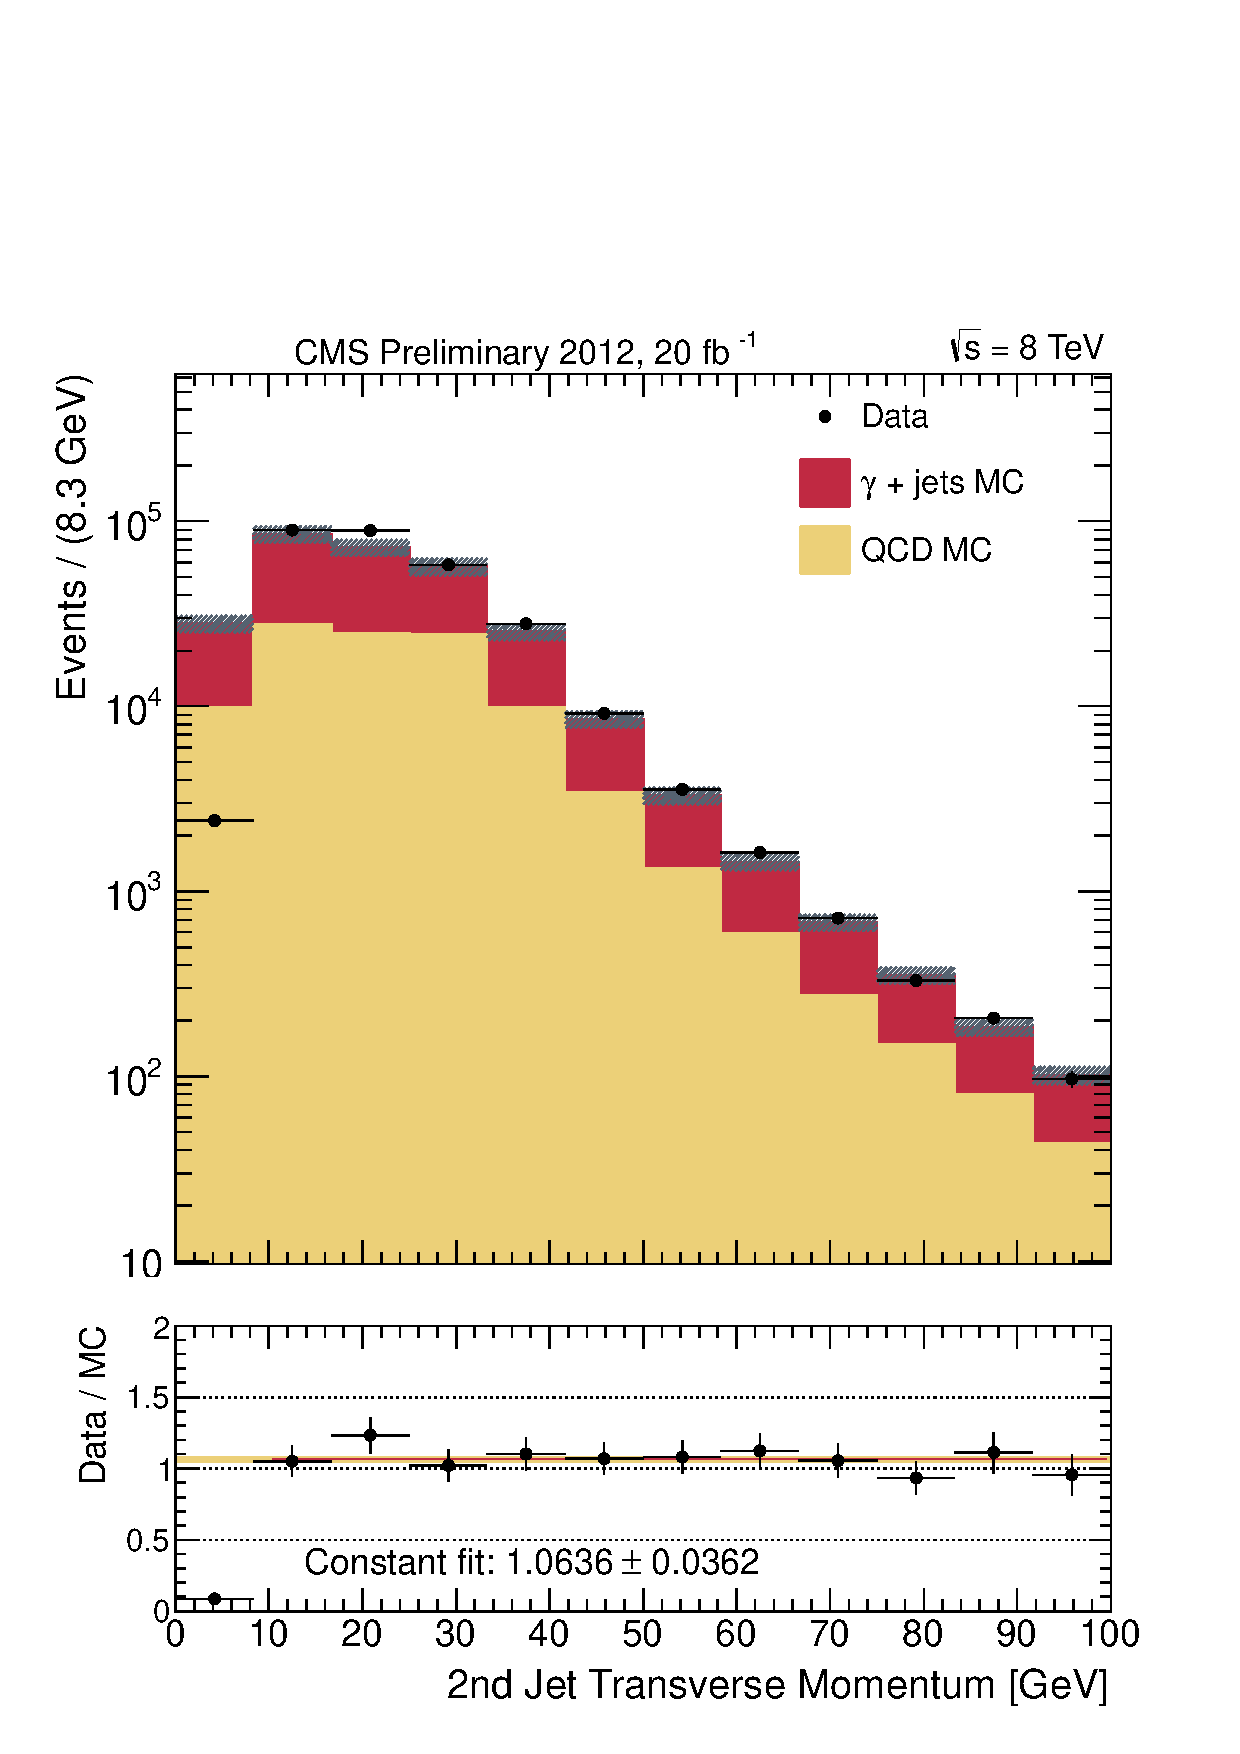
\includegraphics[width=0.45\textwidth]{chapitre4/figs/ptSecondJet_passedID_log.pdf}}\hfill
    \subcaptionbox{\label{met}}[0.45\textwidth]{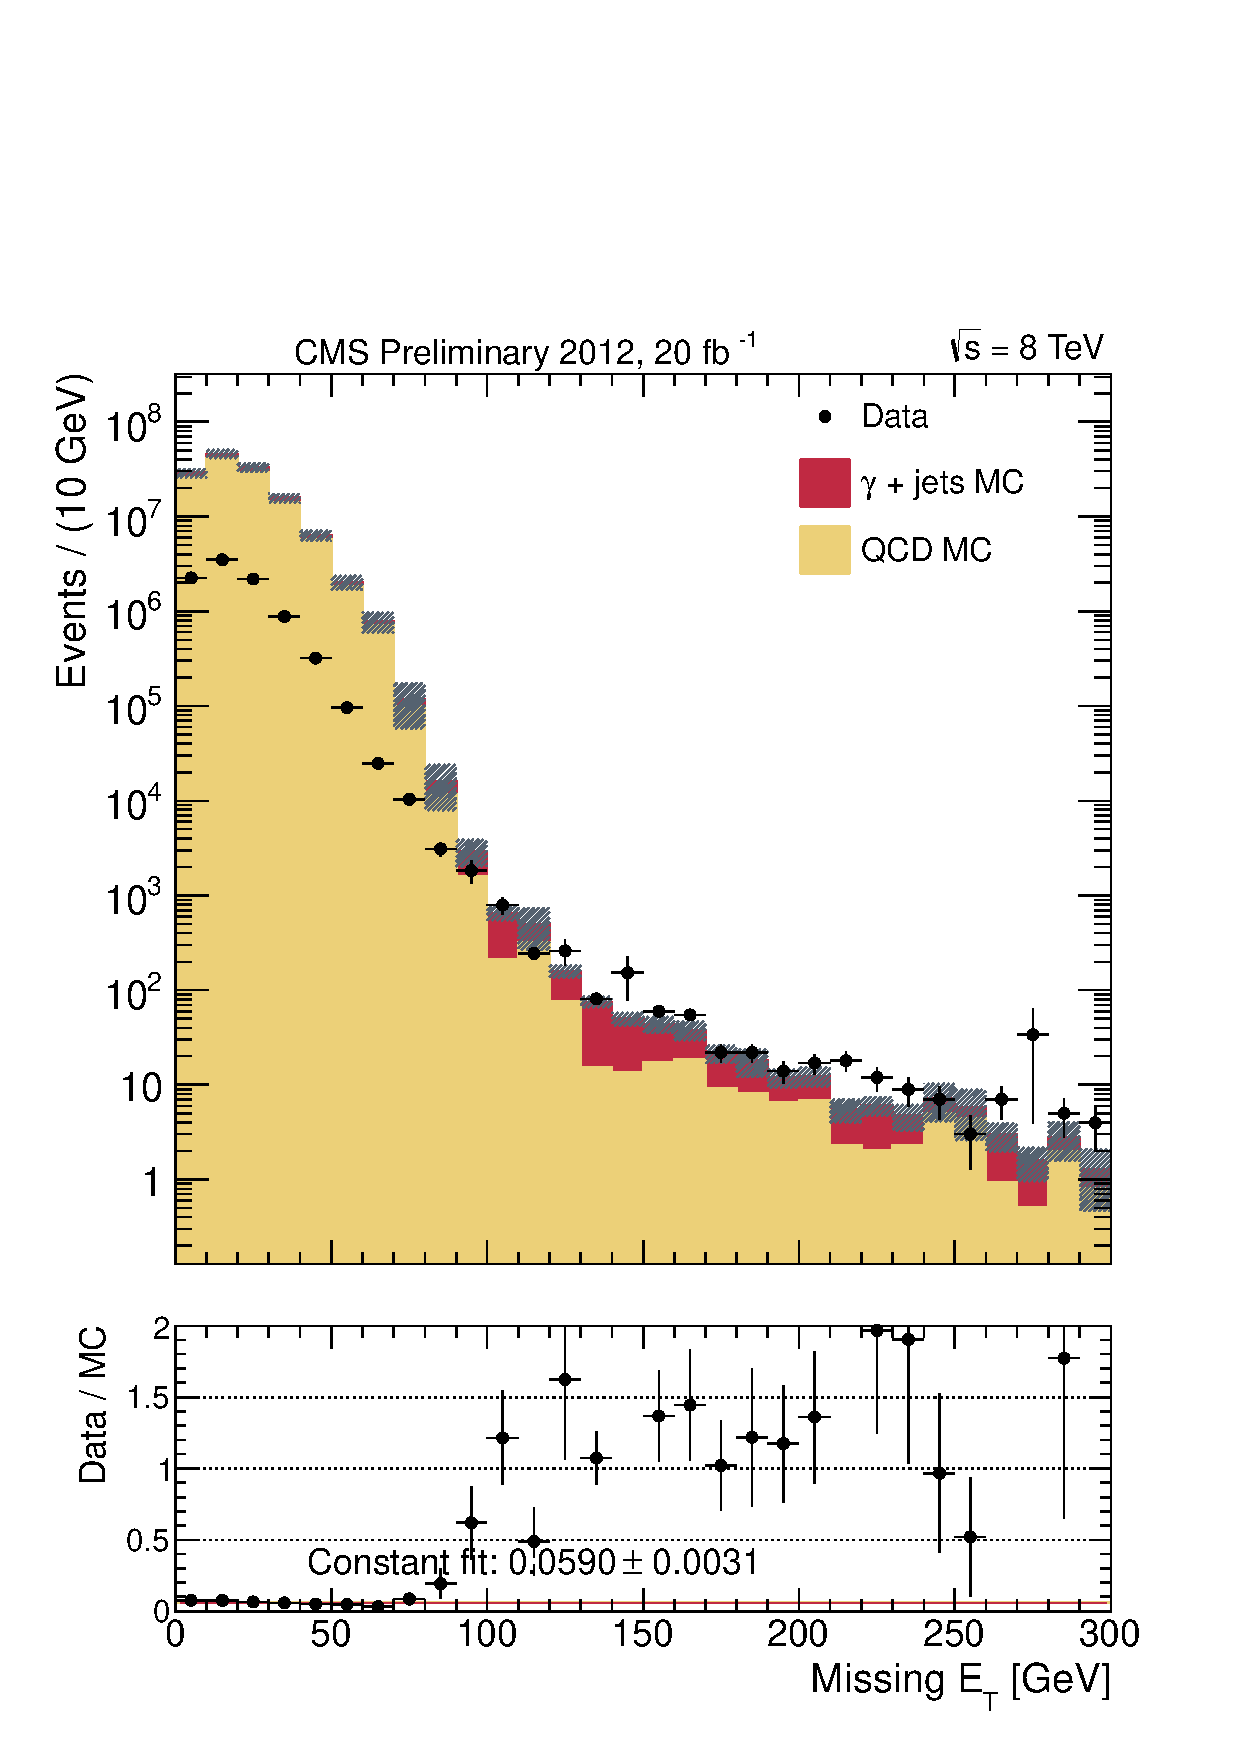
\includegraphics[width=0.45\textwidth]{chapitre4/figs/MET_passedID_log.pdf}}
    \caption{Comparaison entre la simulation (histogrammes) et les données (points) de l'impulsion transverse pour le photon (\subref{pt_photon}), pour le premier jet de l'événement (\subref{pt_first_jet}), le second (\subref{pt_second_jet}) ainsi que pour l'énergie transverse manquante (\subref{met}) après sélection. Une coupure additionnelle sur l'impulsion transverse du photon à \SI{175}{\GeV} a été appliquée pour éviter les effets du facteur de \emph{prescale} des différents chemins de déclenchement (plus de détails \cref{sec:jetmet_strategy}). Ces distributions sont normalisées au nombre d'événements dans les données, et la zone hachurée représente les incertitudes.}
    \label{fig:pt_photon_jet}
\end{figure}

\bigskip

On présente \cref{fig:pt_photon_jet} une comparaison entre la simulation et les données pour l'impulsion transverse du photon, du premier jet de l'événement, du second, ainsi que l'énergie transverse manquante. Les distributions sont normalisées au nombre d'événements dans les données, et l'incertitude sur la simulation comprend l'incertitude statistique, l'incertitude sur la luminosité de \SI{2.6}{\%}, ainsi qu'une incertitude de \SI{10}{\%} sur la valeur des sections efficaces de production \Pphoton + jets et multi-jets. On constate quelques désaccords dans les \cref{pt_first_jet,met}. On considère néanmoins que l'accord est suffisant pour notre analyse, puisque aucune erreur systématique n'est présente dans ces distributions, et qu'à aucun moment ces comparaisons ne sont utilisées dans l'analyse.

\subsection{Stratégie d'analyse} \label{sec:jetmet_strategy}

Les événements sélectionnés sont classés suivant l'impulsion transverse du photon et la position angulaire du jet, afin d'augmenter la sensibilité de l'analyse. 14 classes sont définies en impulsion transverse :

\setlength{\columnsep}{0pt}
\begin{multicols}{4}
  \begin{itemize} \setlength{\itemsep}{0.4\itemsep}
      \item 40 - \SI{50}{\GeV}
      \item 50 - \SI{60}{\GeV}
      \item 60 - \SI{75}{\GeV}
      \item 100 - \SI{125}{\GeV}
      \item 125 - \SI{155}{\GeV}
      \item 155 - \SI{180}{\GeV}
      \item 180 - \SI{210}{\GeV}
      \item 250 - \SI{300}{\GeV}
      \item 300 - \SI{350}{\GeV}
      \item 350 - \SI{400}{\GeV}
      \item 400 - \SI{500}{\GeV}
      \item 500 - \SI{600}{\GeV}
      \item 600 - \SI{800}{\GeV}
      \item 800 - \SI{5000}{\GeV}
  \end{itemize}
\end{multicols}

\begin{table} \centering
  \subcaptionbox{Run ACD\label{tab:triggers_runACD}}[0.45\textwidth]{
  \begin{tabular}{@{}cc@{}} \toprule
    Classes en \ptg & Déclencheurs \\ \midrule
    40 - \SI{60}{\GeV} & \texttt{HLT\_Photon30} \\
    60 - \SI{100}{\GeV} & \texttt{HLT\_Photon50} \\
    100 - \SI{155}{\GeV} & \texttt{HLT\_Photon90} \\
    155 - $\inf$ & \texttt{HLT\_Photon135} \\ \bottomrule
  \end{tabular}
  } \qquad
  \subcaptionbox{Run B\label{tab:triggers_runB}}[0.45\textwidth]{
  \begin{tabular}{@{}cc@{}} \toprule
    Classe en \ptg & Déclencheurs \\ \midrule
    40 - \SI{60}{\GeV} & \texttt{HLT\_Photon30} \\
    60 - \SI{100}{\GeV} & \texttt{HLT\_Photon50} \\
    100 - \SI{155}{\GeV} & \texttt{HLT\_Photon90} \\
    155 - \SI{180}{\GeV} & \texttt{HLT\_Photon135} \\
    180 - $\inf$ & \texttt{HLT\_Photon150} \\ \bottomrule
  \end{tabular}}
  \caption{Chemins de déclenchement associés aux classes en \ptg, pour deux périodes de prises de données correspondantes à des conditions de déclenchement différentes.}
  \label{tab:triggers_jetmet}
\end{table}

À \SI{8}{\TeV} et à l'arbre, un processus $\Pphoton$ + 1 / 2 jets a une section efficace de \SI[allow-number-unit-breaks]{99668 \pm 236}{\pb}. À cause de cette section efficace élevée, les chemins de déclenchement demandant simplement un photon possèdent un facteur de \emph{prescale}. Le seul qui ne l'est pas demande ainsi un photon d'au moins \SI{150}{\GeV}. Afin d'éviter tout biais possible dans l'analyse, chaque classe en \ptg{} a été choisie de façon à être associée de façon exclusive à un chemin de déclenchement précis, tout en ayant, si possible, une efficacité de déclenchement maximale. Par exemple, pour la classe 100 - \SI{125}{\GeV}, on demande à ce que l'événement ait déclenché le chemin demandant un photon d'au moins \SI{90}{\GeV} (\texttt{HLT\_Photon90}). Les \SI{10}{\GeV} de différence entre le seuil du déclencheur et la classe en \pt permettent de tenir compte des possibles corrections en énergie entre le photon reconstruit au niveau HLT et le photon \pf. À partir de \SI{155}{\GeV} (ou \SI{180}{\GeV} pour une période spécifique de prise de données), tous les événements doivent déclencher le premier chemin ayant un facteur de \emph{prescale} de 1. Le \cref{tab:triggers_jetmet} résume les chemins de déclenchement associés à chaque classe en \ptg. Les chemins de déclenchement ayant changé pendant la période de prise de données (notamment avec l'apparition puis la disparition du déclencheur \texttt{HLT\_Photon150}), deux tableaux sont présents, un pour chaque période de prise de données.

Les facteurs de \emph{prescale} des chemins de déclenchement vont aussi affecter les distributions de \pu associées. Ainsi, lors de la procédure de repondération du \pu sur la simulation, il faut tenir compte du déclencheur associé à l'événement. En fonction de l'impulsion transverse du photon dans les événement simulés, on détermine quel chemin de déclenchement l'événement aurait dû déclencher sur les données pour passer la sélection, et on utilise cette information pour obtenir le profil de \pu correspondant. On présente \cref{fig:pu_jetmet} une comparaison entre deux profils de \pu, obtenus pour deux chemins de déclenchement différents. On voit très clairement la différence entre les deux profils.

\begin{figure}[tbp]
    \centering
    \includegraphics[width=0.5\textwidth]{chapitre4/figs/pu_plot.pdf}
    \caption{Distribution du nombre moyen d'interactions par croisement de faisceaux pour deux chemins de déclenchement, \texttt{HLT\_Photon30} (rouge) et \texttt{HLT\_Photon150} (bleu)}
    \label{fig:pu_jetmet}
\end{figure}

\bigskip

On procède également à une classification selon $\aeta$ du jet, en 7 classes :

\begin{multicols}{4}
  \begin{itemize} \setlength{\itemsep}{0.4\itemsep}
      \item \num{0} - \num{0.8}
      \item \num{0.8} - \num{1.3}
      \item \num{1.3} - \num{1.9}
      \item \num{1.9} - \num{2.5}
      \item \num{2.5} - \num{3}
      \item \num{3} - \num{3.2}
      \item \num{3.2} - \num{5.2}
  \end{itemize}
\end{multicols}

\begin{figure}[p]
    \centering
    \subcaptionbox{\label{fig:bal_eta013_pt_125_155}}[0.45\textwidth]{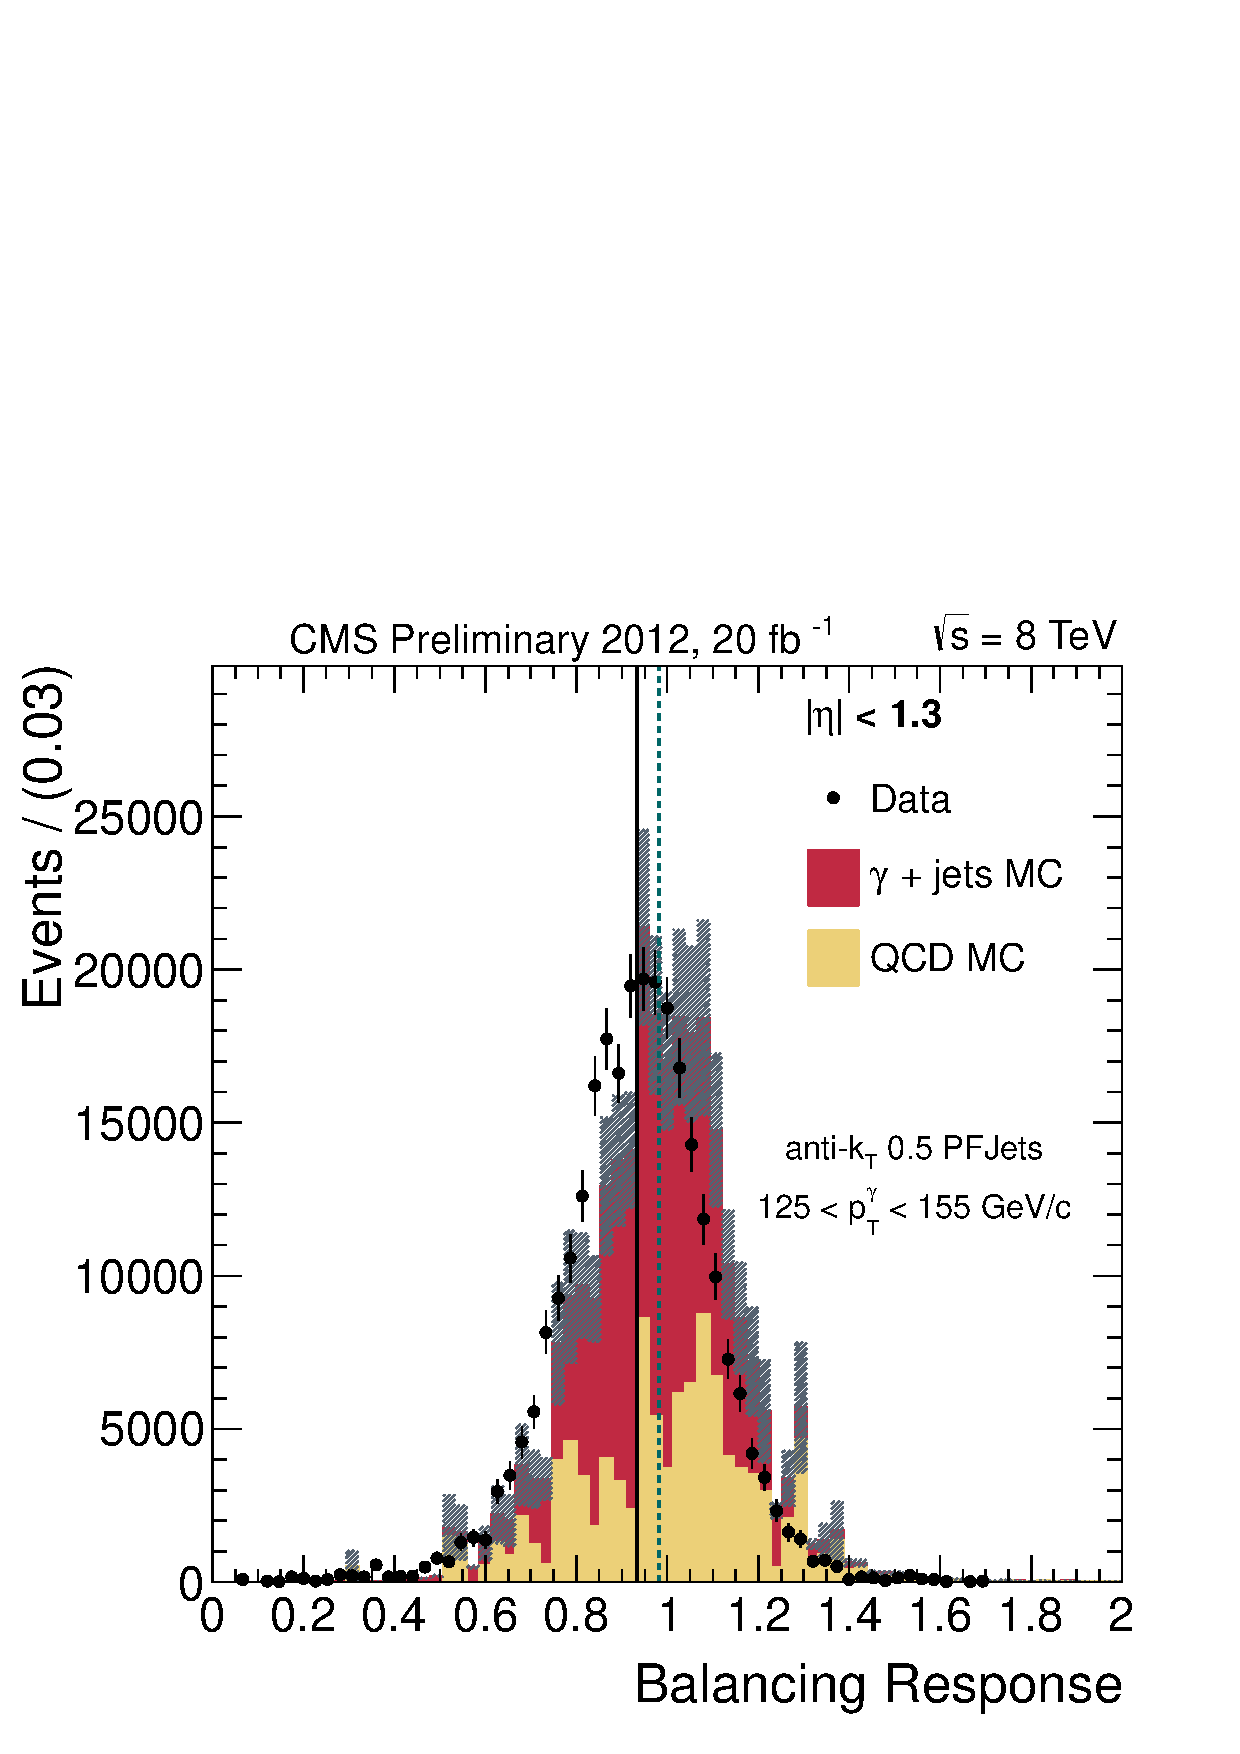
\includegraphics[width=0.45\textwidth]{chapitre4/figs/resp_balancing_eta013_ptPhot_125_155.pdf}}\hfill
    \subcaptionbox{\label{fig:bal_eta013_pt_210_250}}[0.45\textwidth]{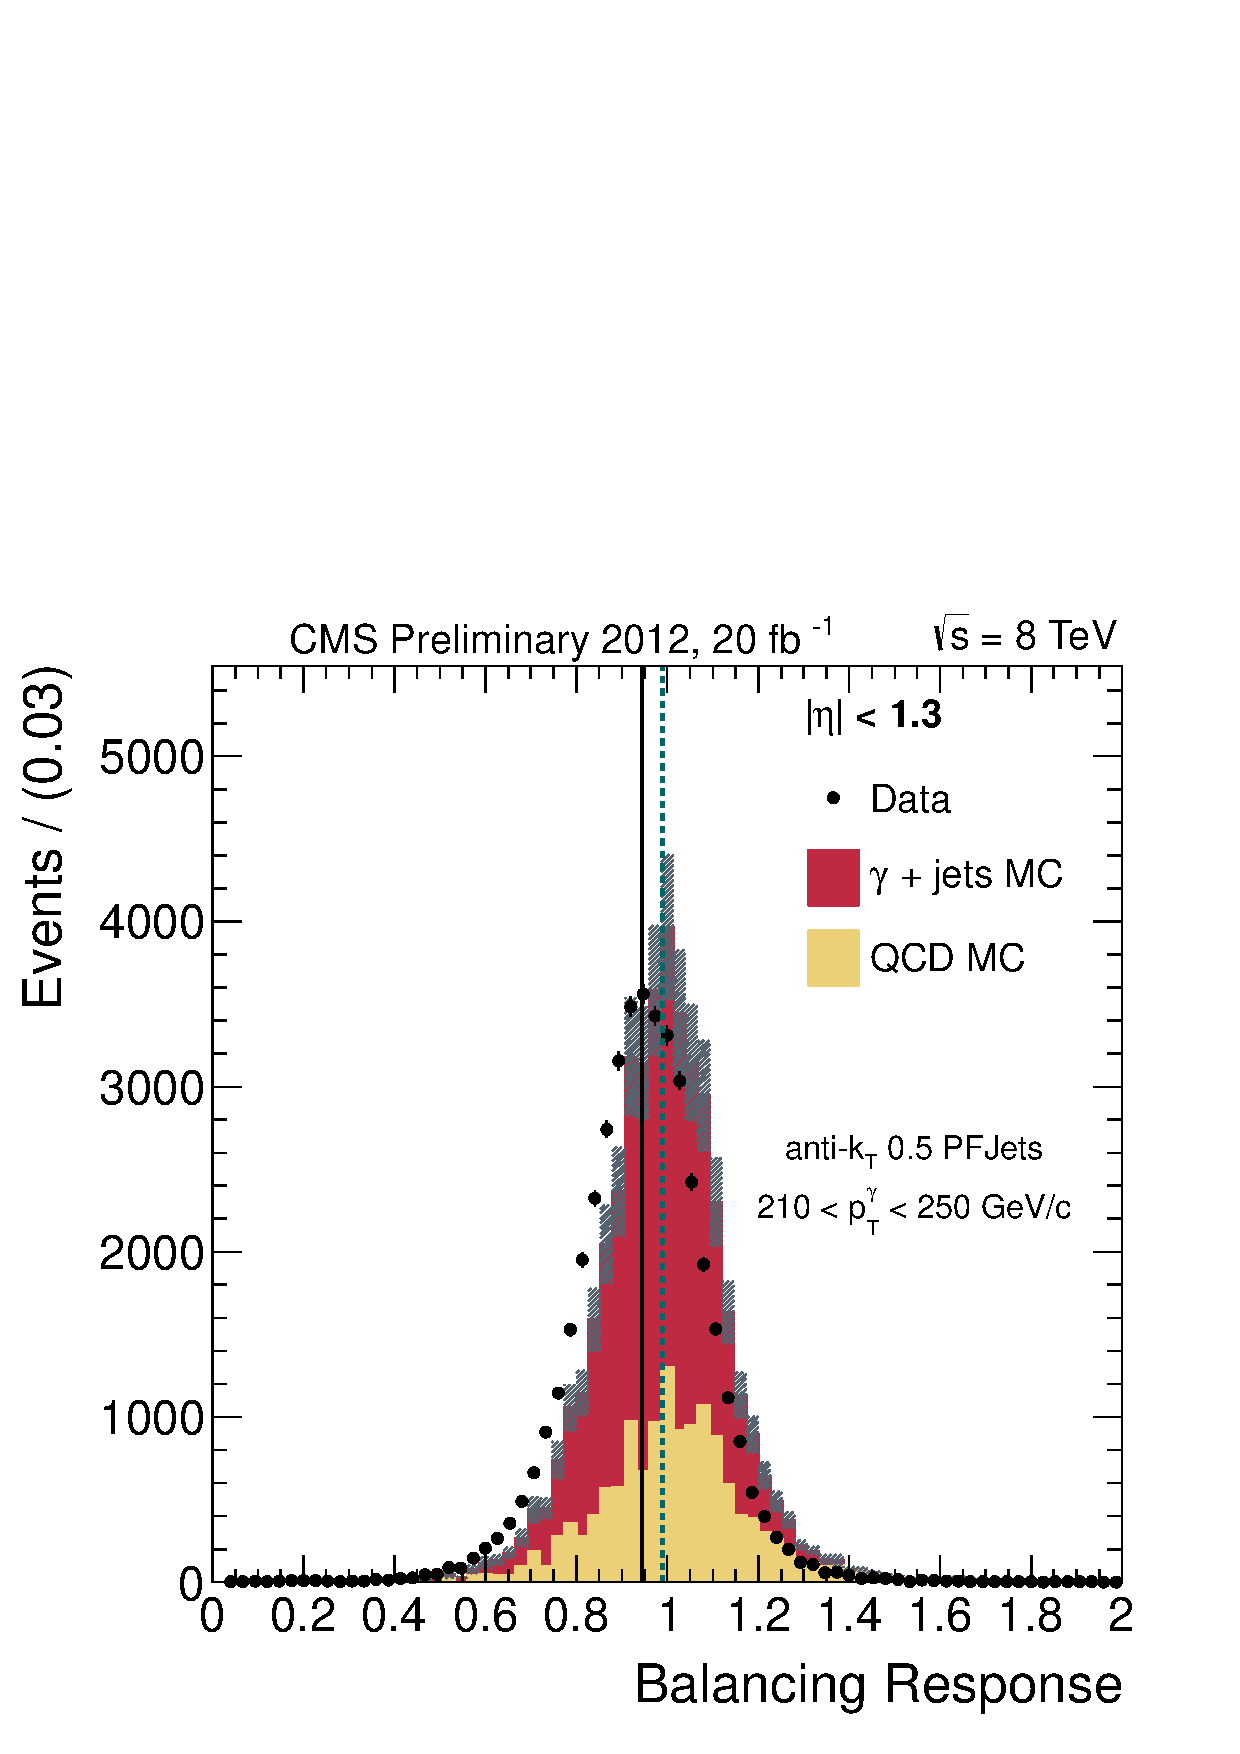
\includegraphics[width=0.45\textwidth]{chapitre4/figs/resp_balancing_eta013_ptPhot_210_250.pdf}}
    \subcaptionbox{\label{fig:mpf_eta013_pt_125_155}}[0.45\textwidth]{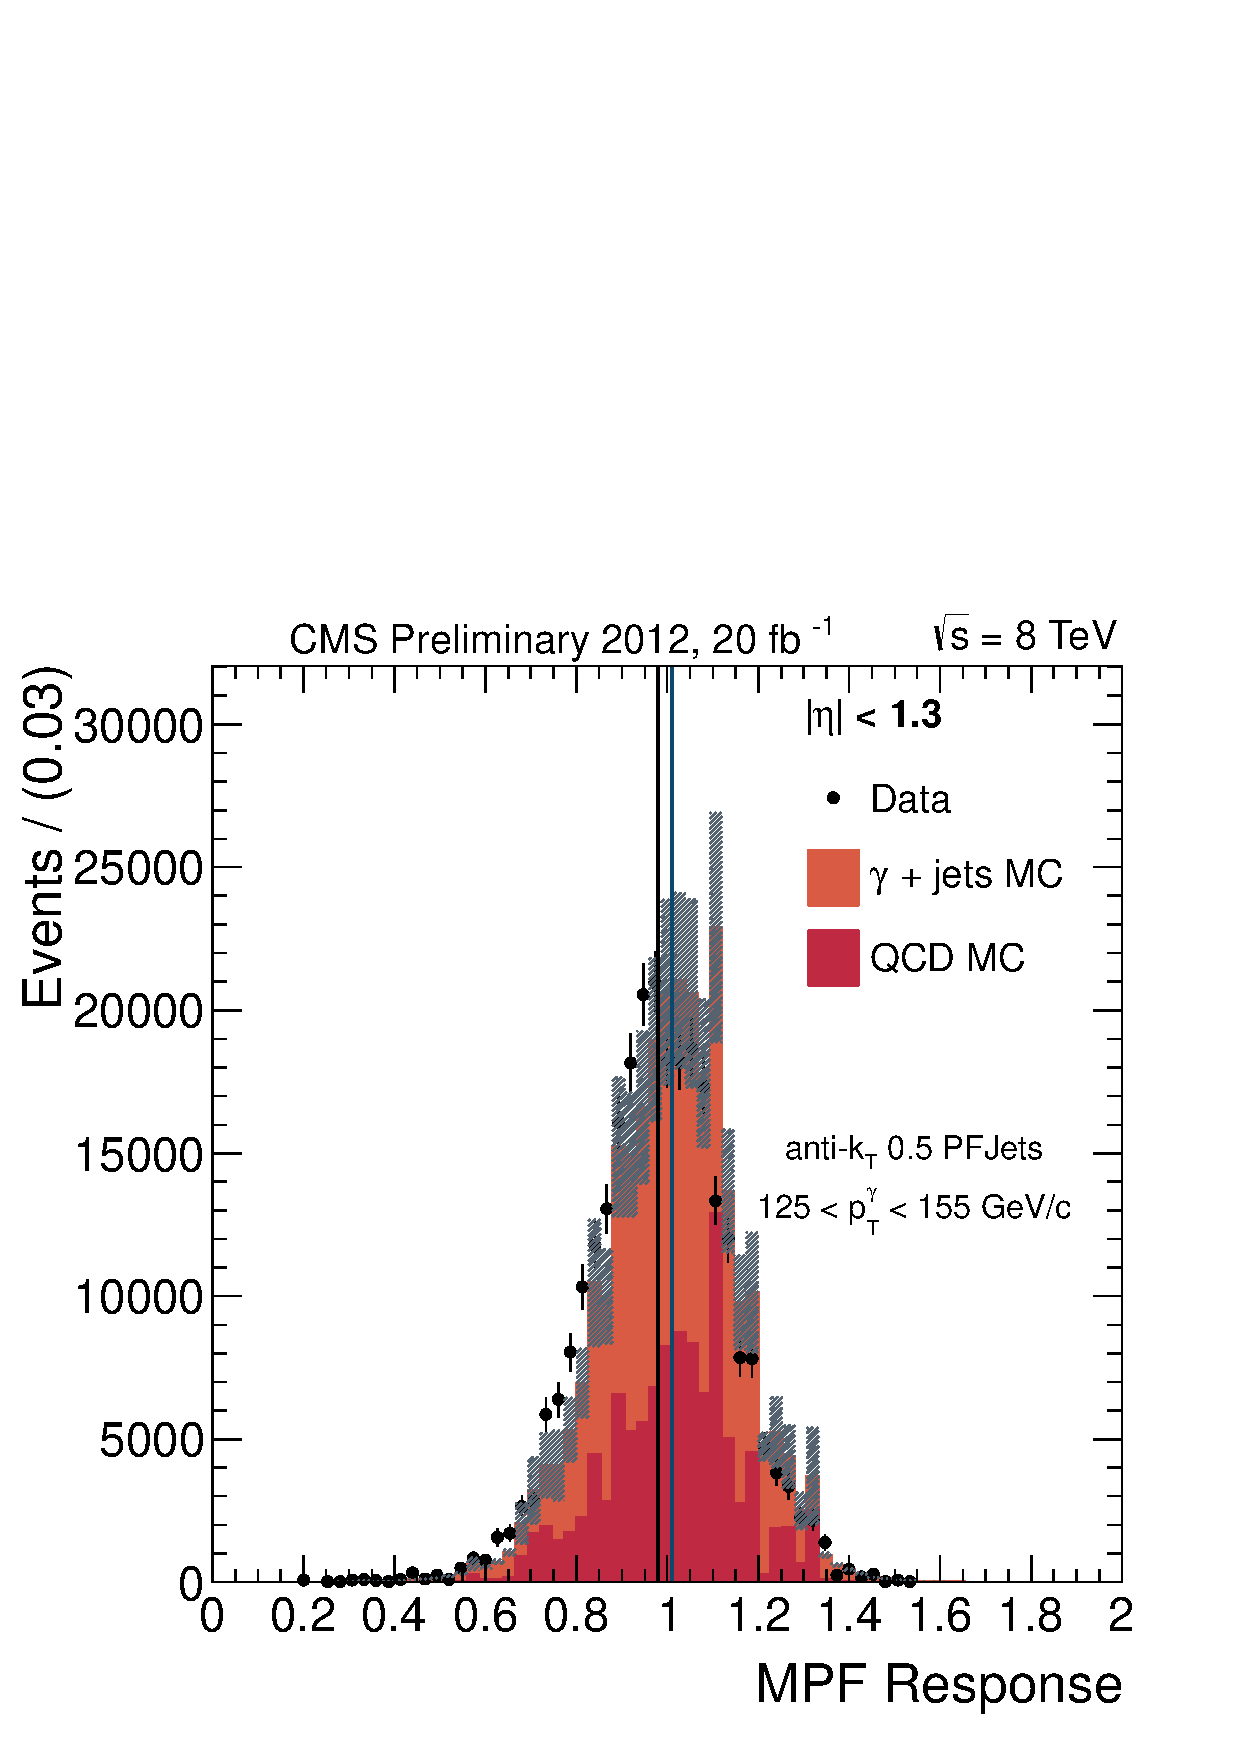
\includegraphics[width=0.45\textwidth]{chapitre4/figs/resp_mpf_eta013_ptPhot_125_155.pdf}}\hfill
    \subcaptionbox{\label{fig:mpf_eta013_pt_210_250}}[0.45\textwidth]{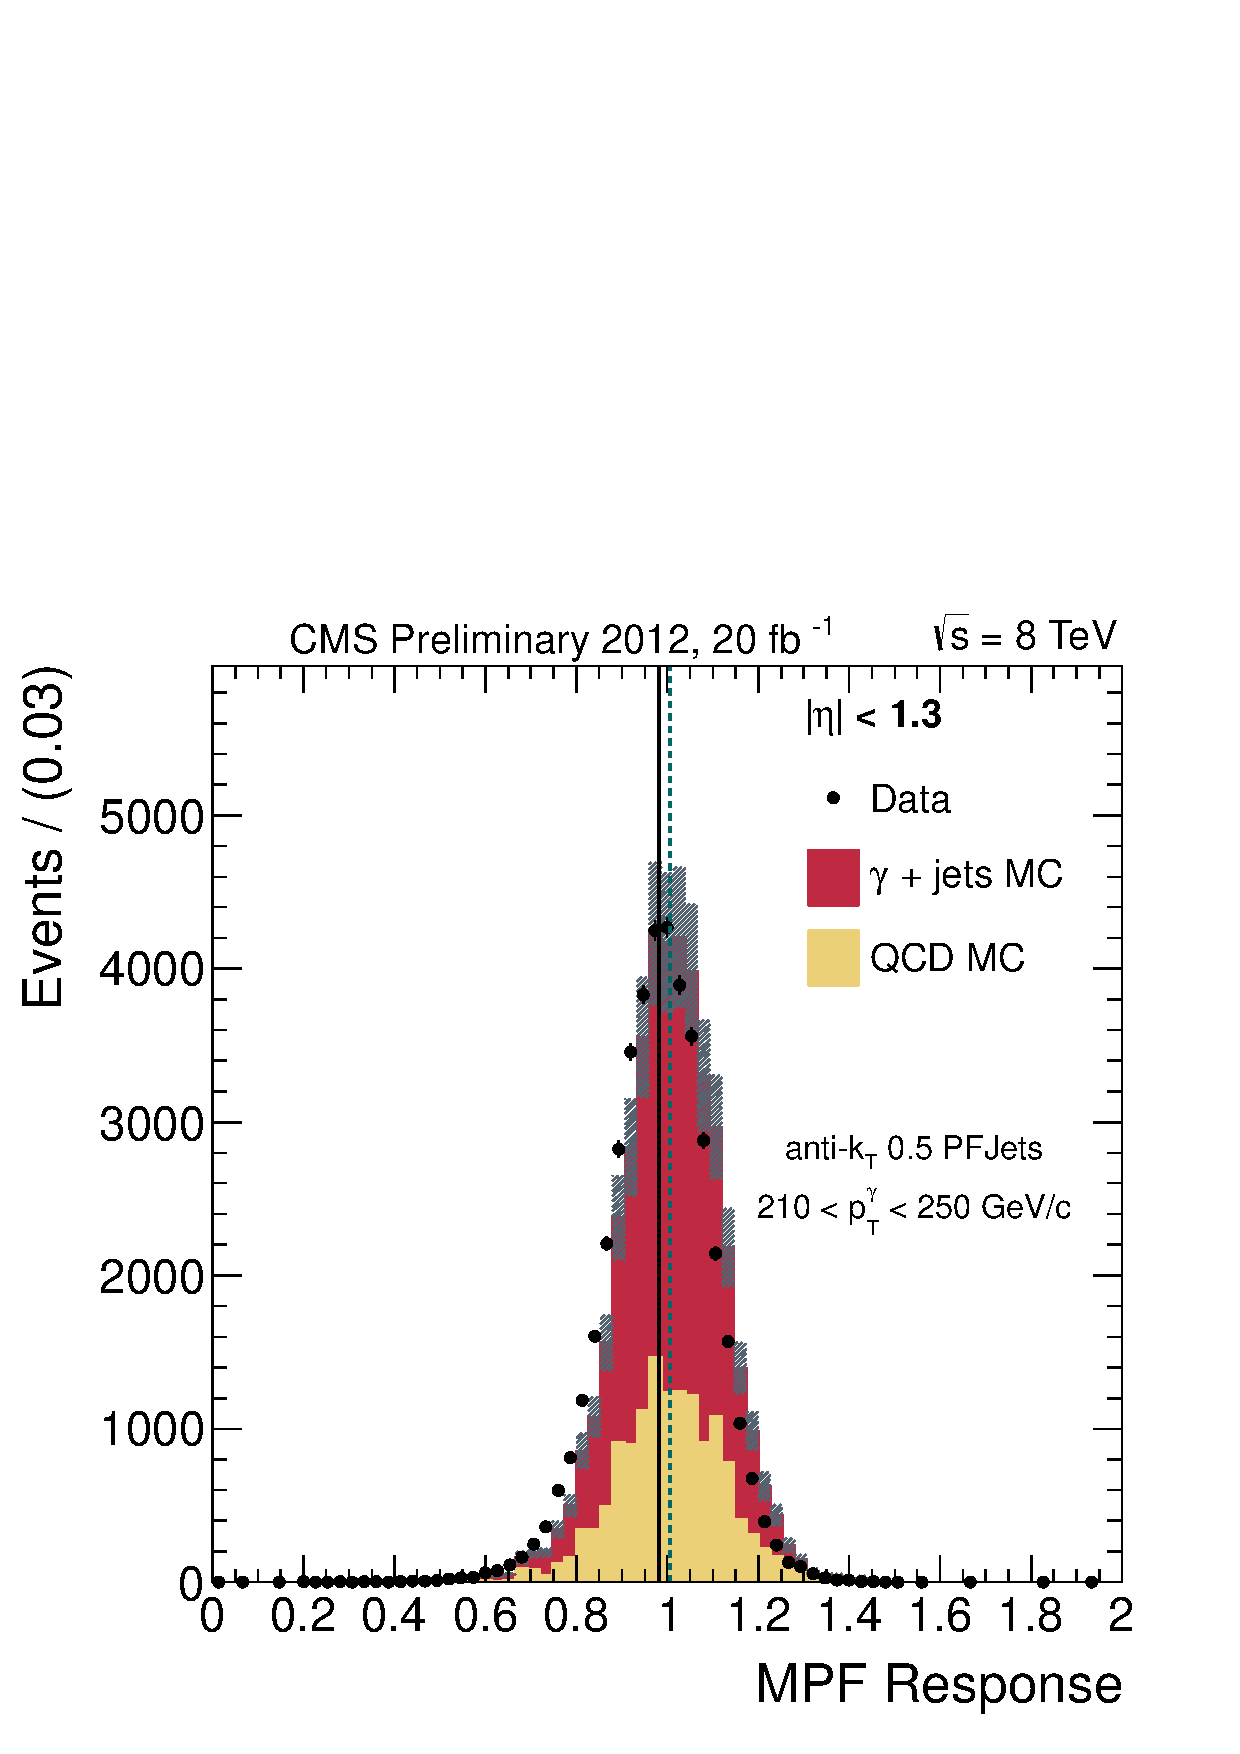
\includegraphics[width=0.45\textwidth]{chapitre4/figs/resp_mpf_eta013_ptPhot_210_250.pdf}}
    \caption{Réponses pour la méthode de la balance (haut) et pour la méthode MPF (bas), pour deux classes en \pt : 125 - \SI{155}{\GeV} (gauche) et 210 - \SI{250}{\GeV} (droite). Pour toutes les distributions, $\aeta < \num{1.3}$. Les histogrammes représentent la simulation et les points les données. La ligne noire correspond à la réponse moyenne $R_m$ extraite sur les données et la ligne bleue celle extraite sur la simulation. Les distributions sont normalisées à la luminosité, et la zone hachurée représente les incertitudes.}
    \label{fig:responses_mpf_balancing}
\end{figure}

Pour chaque classe en $p_T^{\gamma}$ et $\aeta$, on calcule la réponse en utilisant la méthode de la balance et la méthode MPF, sur les données et sur la simulation. On présente \cref{fig:responses_mpf_balancing} les distributions des réponses obtenues pour les deux méthodes, pour diverses classes en \pt, et pour $\aeta < \num{1.3}$. Pour chaque classe, on extrait la réponse moyenne $R_m$, définie comme la moyenne de la distribution des réponses, ainsi que la résolution $\sigma$, définie comme la moyenne quadratique de la distribution des réponses (RMS) divisée par $R_m$. Sur chaque distribution représentée \cref{fig:responses_mpf_balancing}, les réponses moyennes sont représentées par une ligne noire pour les données, et par une ligne bleue pour la simulation. On constate que ces réponses sont différentes, et c'est ce biais que l'on souhaite corriger en appliquant les corrections résiduelles.

\subsection{Résultats} \label{sec:jetmet_results}

Pour chaque distribution des réponses, on extrait la réponse moyenne et la résolution. Afin d'extraire les corrections résiduelles, on trace l'évolution de $R_m$ en fonction de l'impulsion transverse du photon, pour les données et la simulation, pour différentes classes en \aeta. En calculant le rapport entre données et simulation, on détermine le facteur de correction à appliquer sur les données.

On définit le facteur de correction $f$ par
\begin{align*}
  f &= \frac{R_m^{\text{simulation}}}{R_m^{\text{données}}}
\end{align*}

En appliquant ce facteur de correction sur les données, on a
\begin{align*}
  f\;R_m^{\text{données}} &= R_m^{\text{simulation}}
\end{align*}
ce qui est effectivement le but recherché.

\bigskip

On présente par la suite les résultats obtenus avec les méthodes de la balance et MPF, avec et sans extrapolation, qui permettent d'extraire le facteur de correction résiduel. Pour chaque méthode, les distributions des réponses moyennes seront présentées pour différentes classes en \aeta.

\subsubsection{Méthode de la balance, sans extrapolation}

On présente \cref{fig:balancing_resp} les distributions des réponses moyennes pour différentes classes en \aeta. Le ratio entre les données et la simulation accompagne ces distributions, ce qui permet d'extraire les facteurs de corrections. Pour ce faire, une interpolation linéaire par une constante est dérivée à l'aide des divers ratios.
% On trouve aussi \cref{fig:balancing_reso} les distributions des résolutions pour les mêmes classes en \aeta. Même si ces résolutions ne sont pas utilisées pour dériver les corrections résiduelles, elles sont intéressantes pour se rendre compte des performances de reconstruction des algorithmes. On s'aperçoit d'ailleurs que les jets sont mieux reconstruits sur la simulation que sur les données. Cet effet donne lieu à une autre série de corrections pour la résolution, qui vise à dégrader la résolution des jets sur la simulation pour correspondre à celle des données.

\begin{figure}[p]
    \centering
    \subcaptionbox{\label{fig:bal_eta008}}[0.45\textwidth]{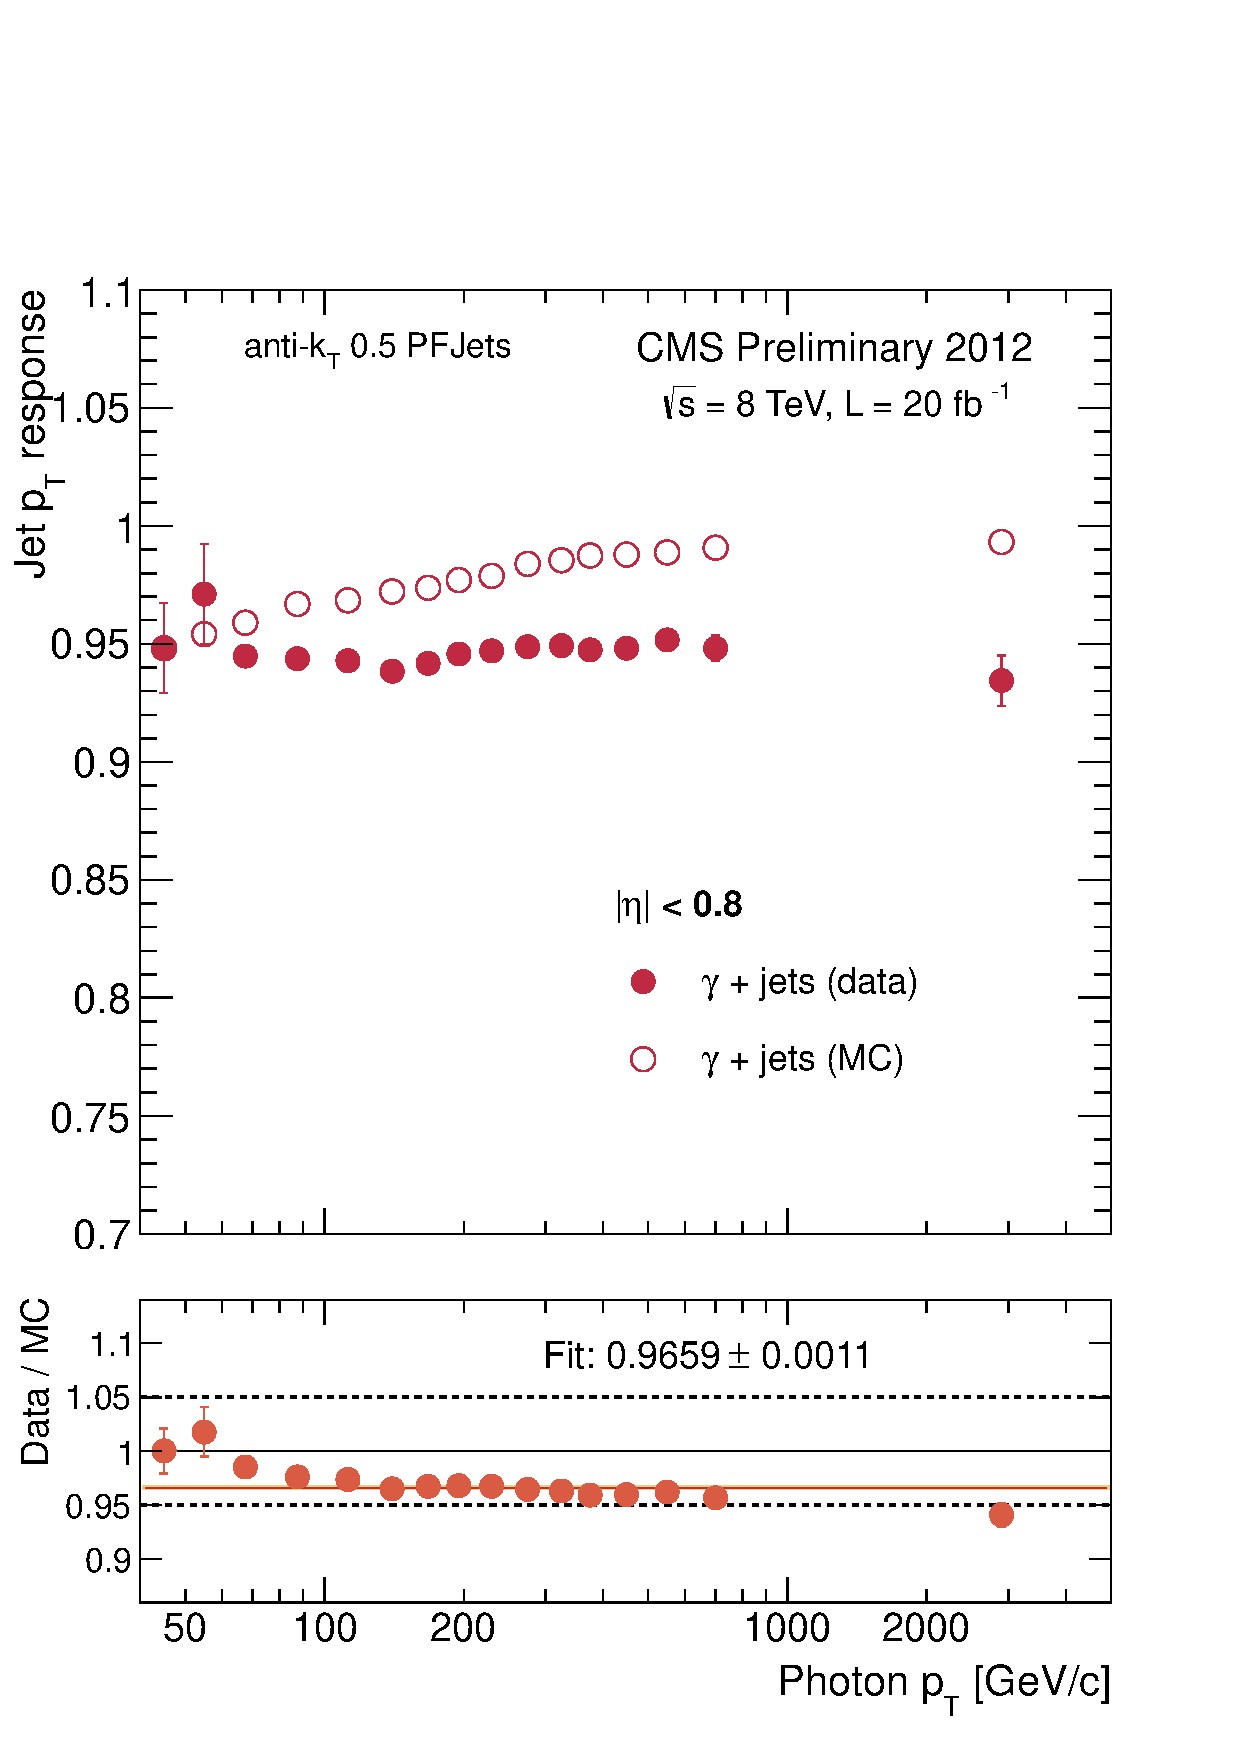
\includegraphics[width=0.45\textwidth]{chapitre4/figs/resp_balancing/response_eta008_balancing.pdf}}\hfill
    \subcaptionbox{\label{fig:bal_eta0813}}[0.45\textwidth]{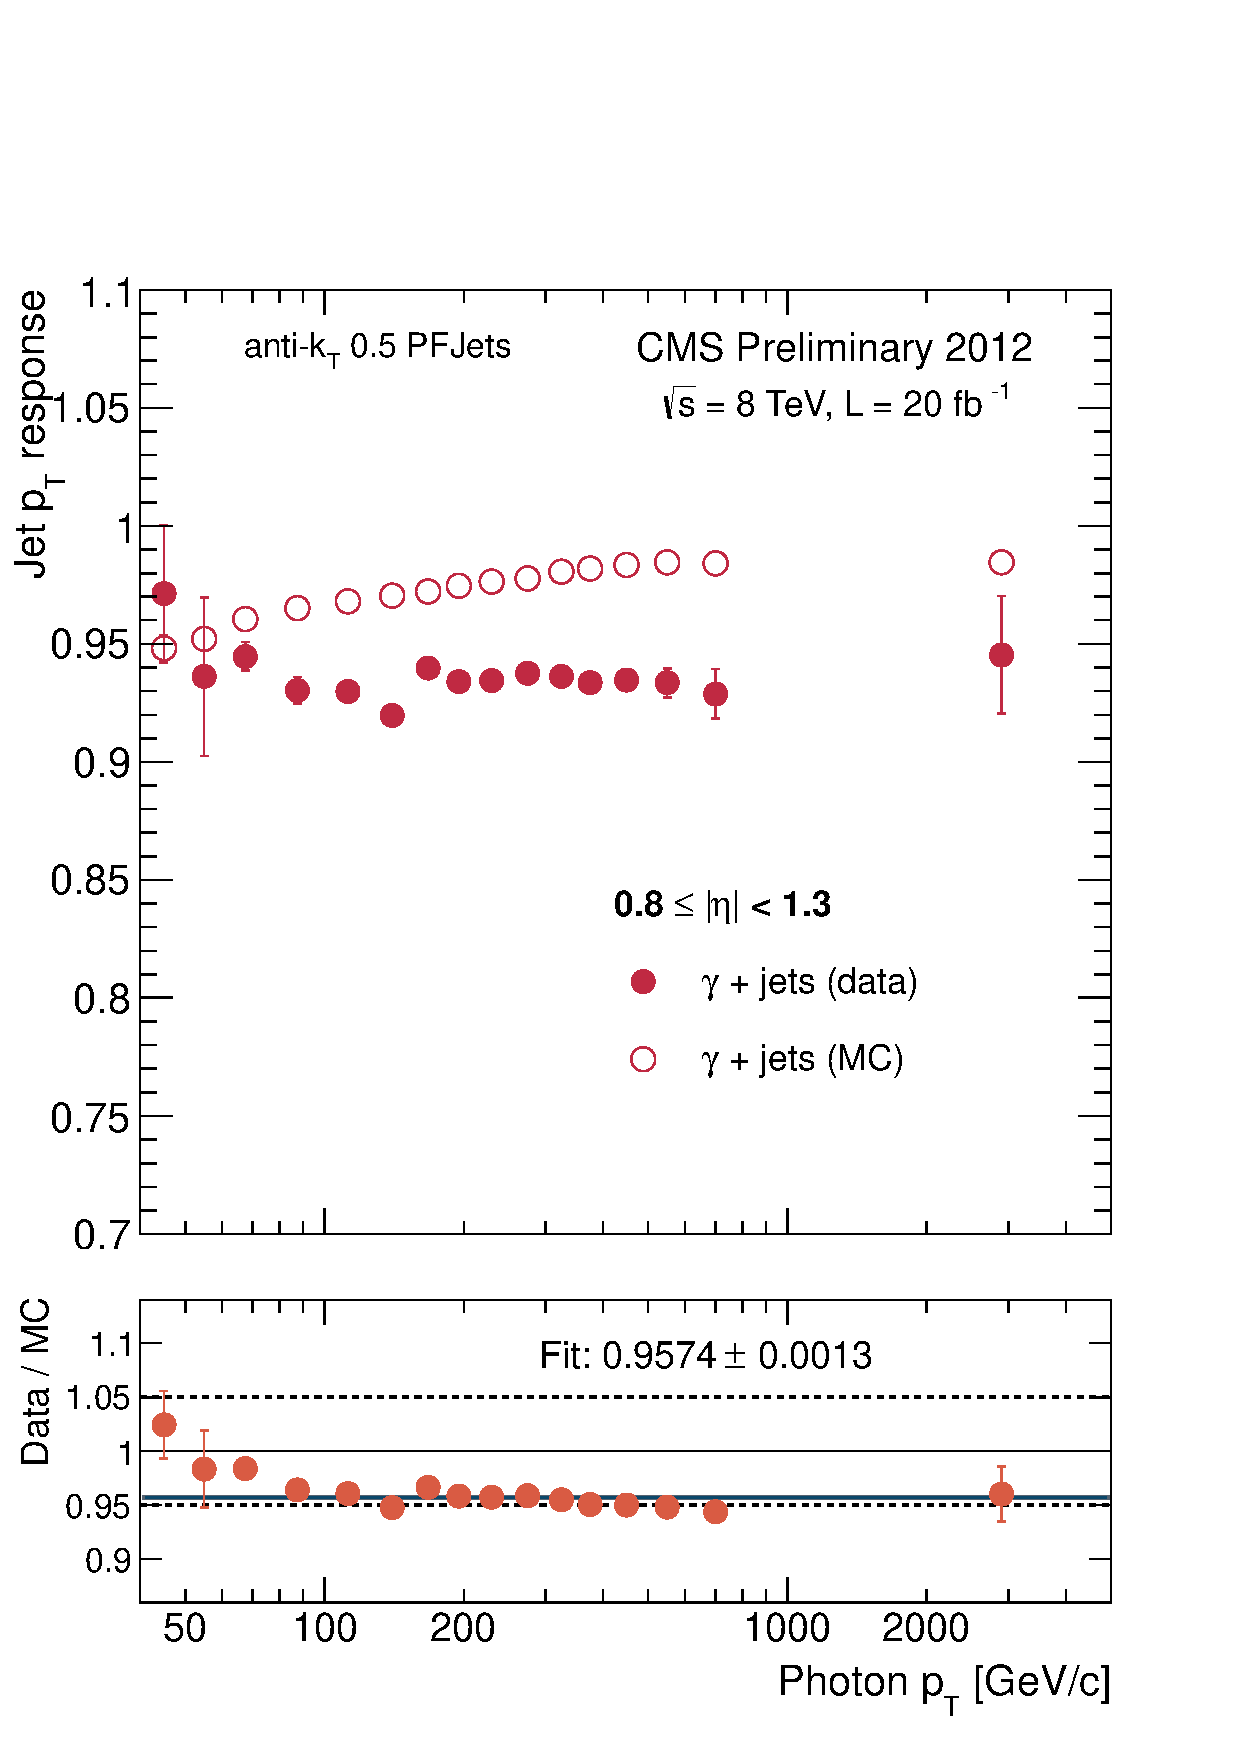
\includegraphics[width=0.45\textwidth]{chapitre4/figs/resp_balancing/response_eta0813_balancing.pdf}}
    \subcaptionbox{\label{fig:bal_eta1319}}[0.45\textwidth]{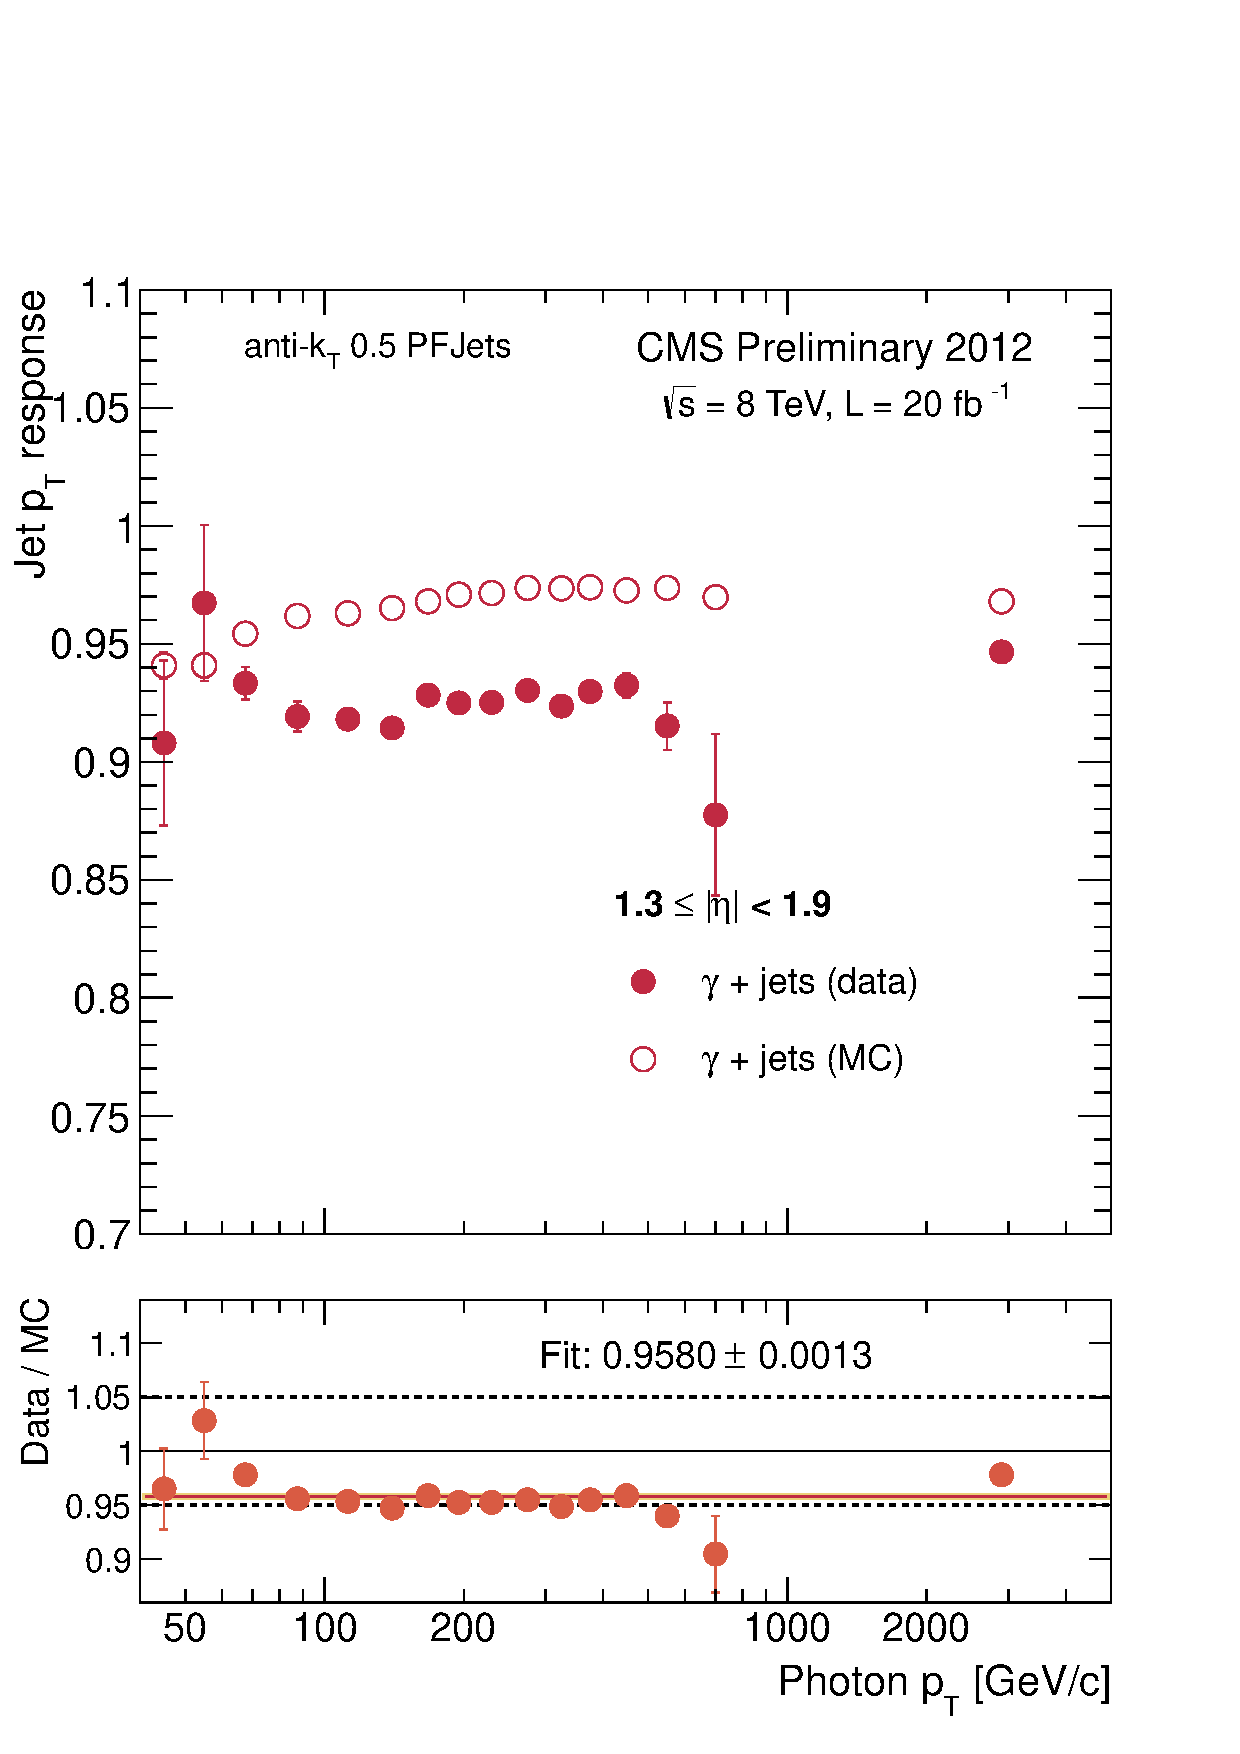
\includegraphics[width=0.45\textwidth]{chapitre4/figs/resp_balancing/response_eta1319_balancing.pdf}}\hfill
    \subcaptionbox{\label{fig:bal_eta1925}}[0.45\textwidth]{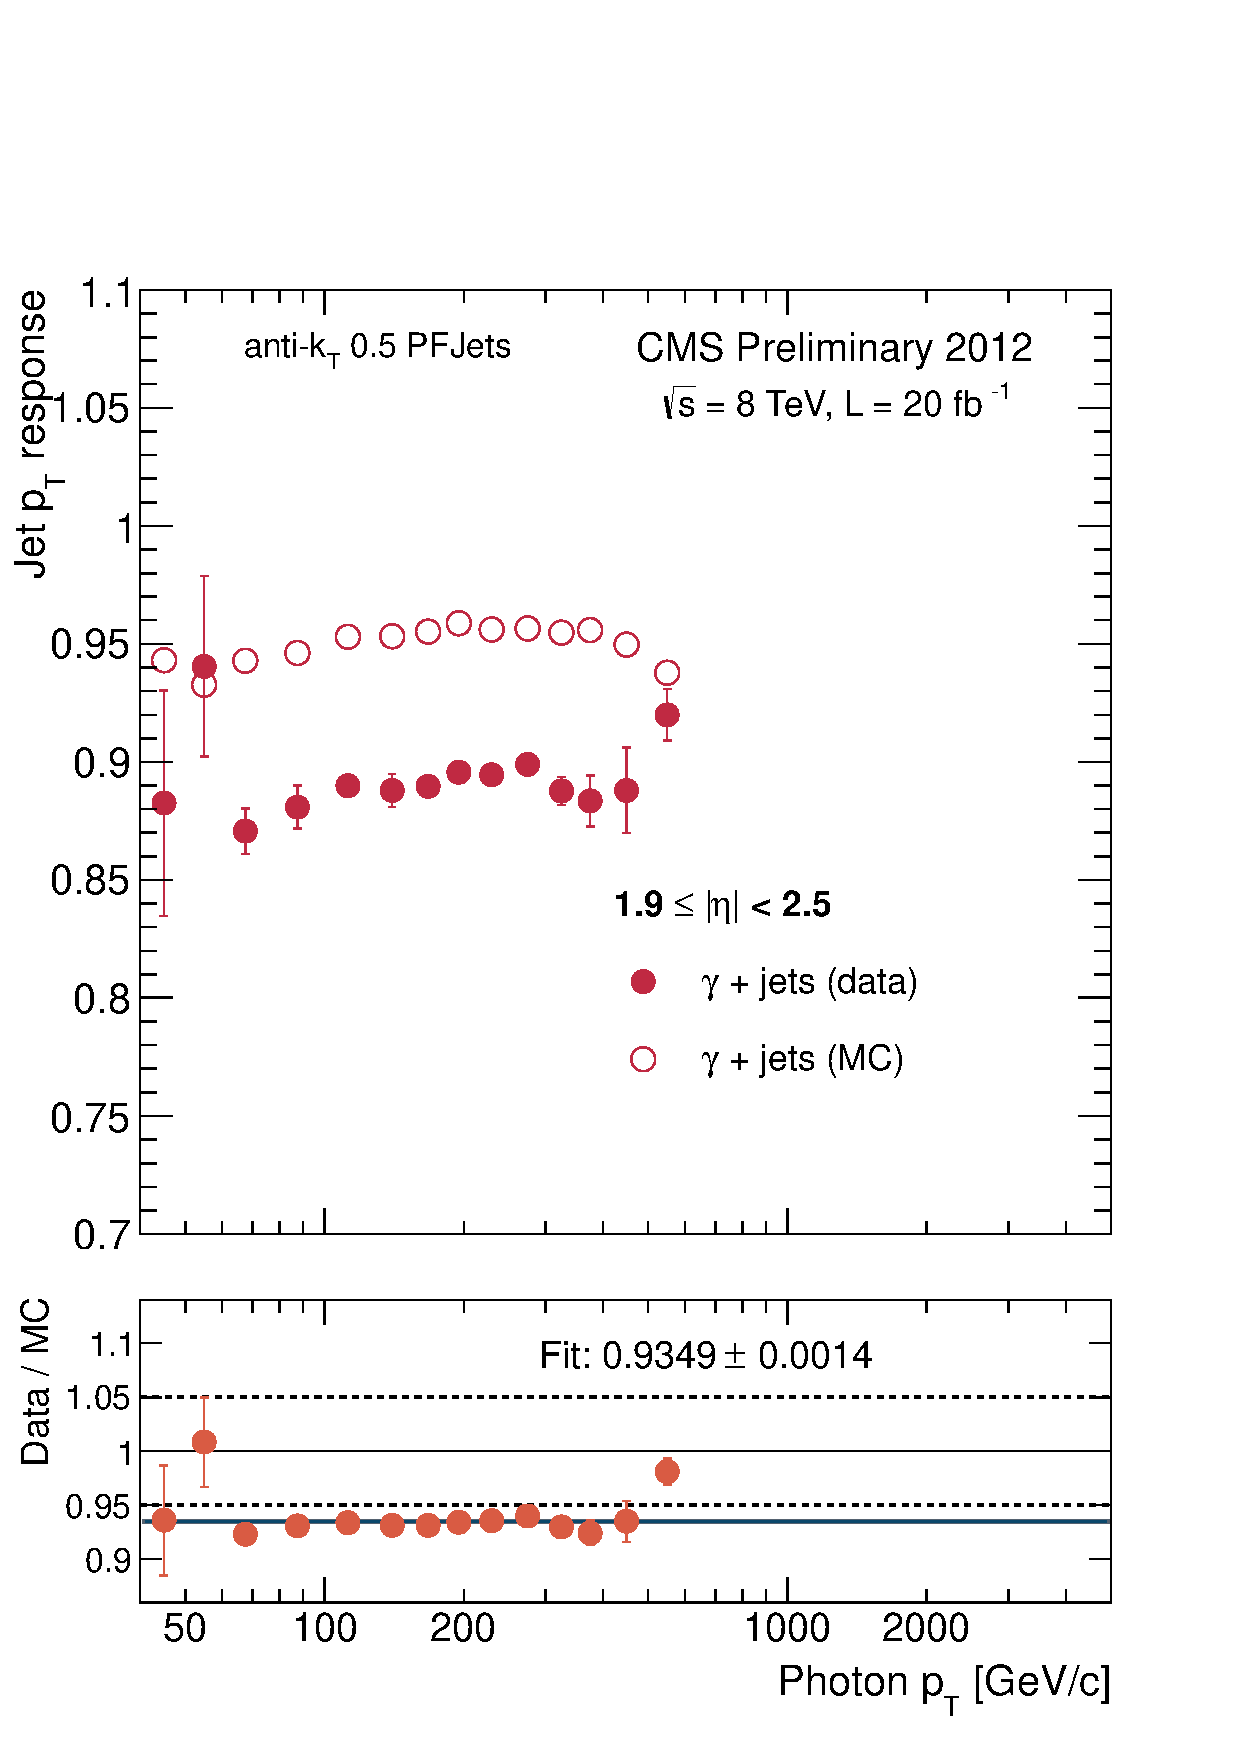
\includegraphics[width=0.45\textwidth]{chapitre4/figs/resp_balancing/response_eta1925_balancing.pdf}}
    \caption{Réponses moyennes pour la méthode de la balance pour $\aeta < \num{0.8}$ (\subref{fig:bal_eta008}), $\num{0.8} \leq \aeta < \num{1.3}$ (\subref{fig:bal_eta0813}), $\num{1.3} \leq \aeta < \num{1.9}$ (\subref{fig:bal_eta1319}), et $\num{1.9} \leq \aeta < \num{2.5}$ (\subref{fig:bal_eta1925}). Le ratio entre les données et la simulation est présenté sous chaque distribution, accompagné d'une interpolation linéaire constante (ligne orange). La bande jaune représente l'erreur sur cette interpolation.}
    \label{fig:balancing_resp}
\end{figure}

% \begin{figure}[p]
%     \centering
%     \subcaptionbox{\label{fig:reso_bal_eta008}}[0.45\textwidth]{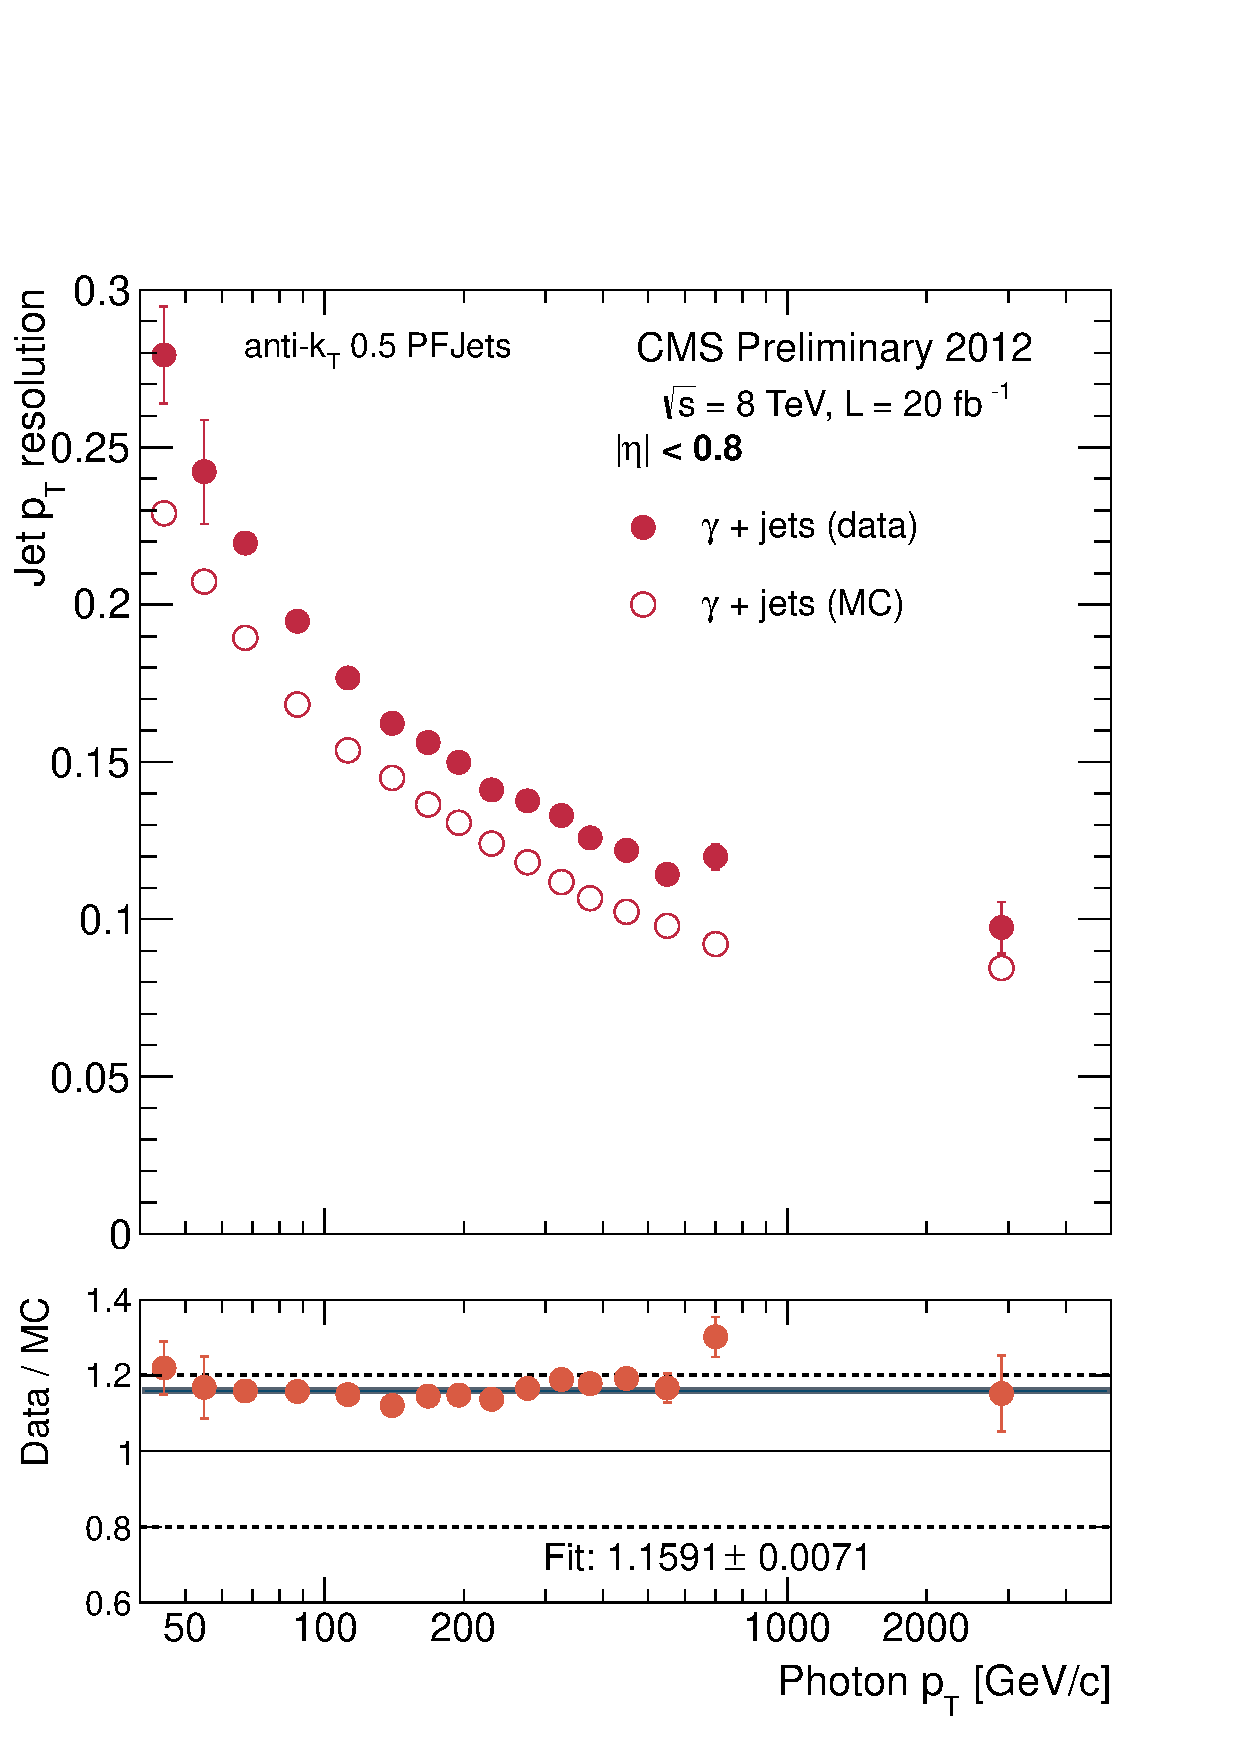
\includegraphics[width=0.45\textwidth]{chapitre4/figs/reso_balancing/resolution_eta008_balancing.pdf}}\hfill
%     \subcaptionbox{\label{fig:reso_bal_eta0813}}[0.45\textwidth]{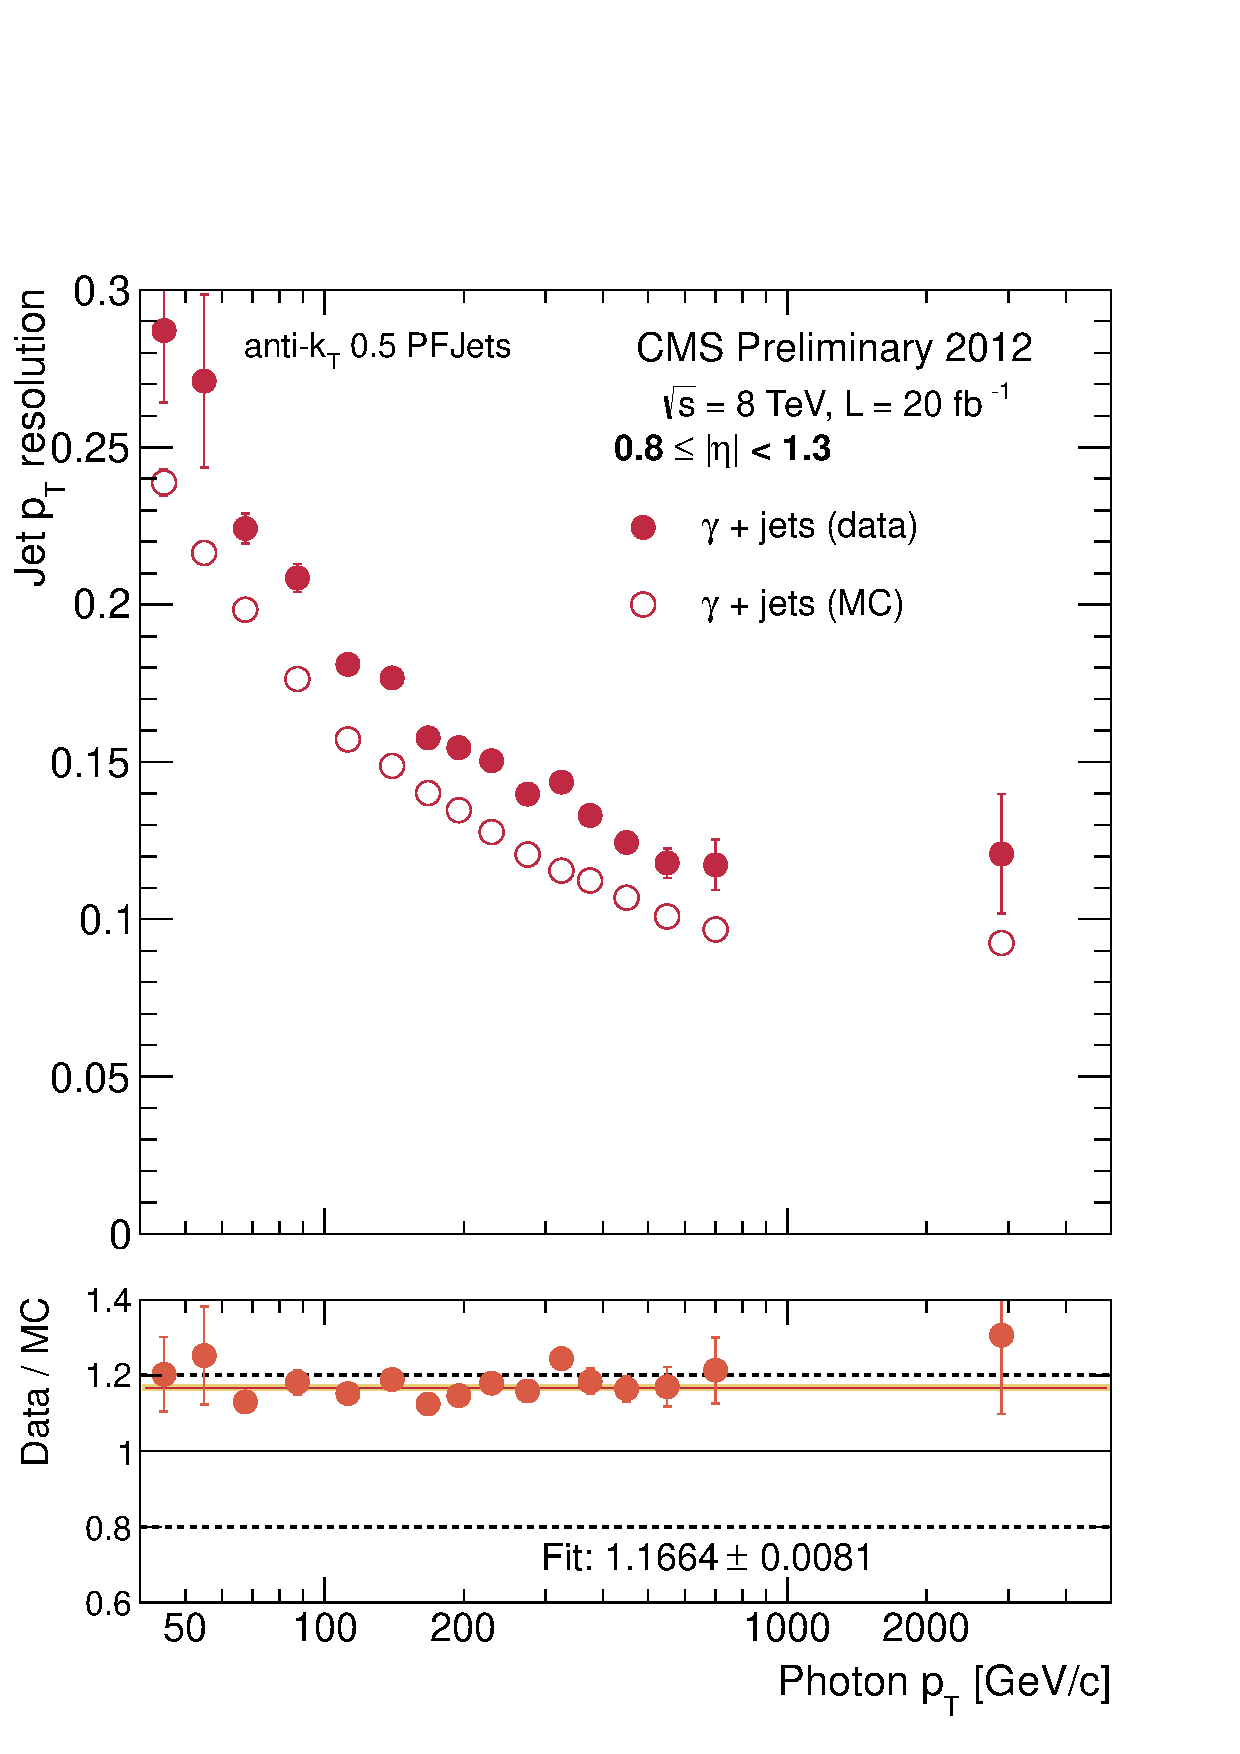
\includegraphics[width=0.45\textwidth]{chapitre4/figs/reso_balancing/resolution_eta0813_balancing.pdf}}
%     \subcaptionbox{\label{fig:reso_bal_eta1319}}[0.45\textwidth]{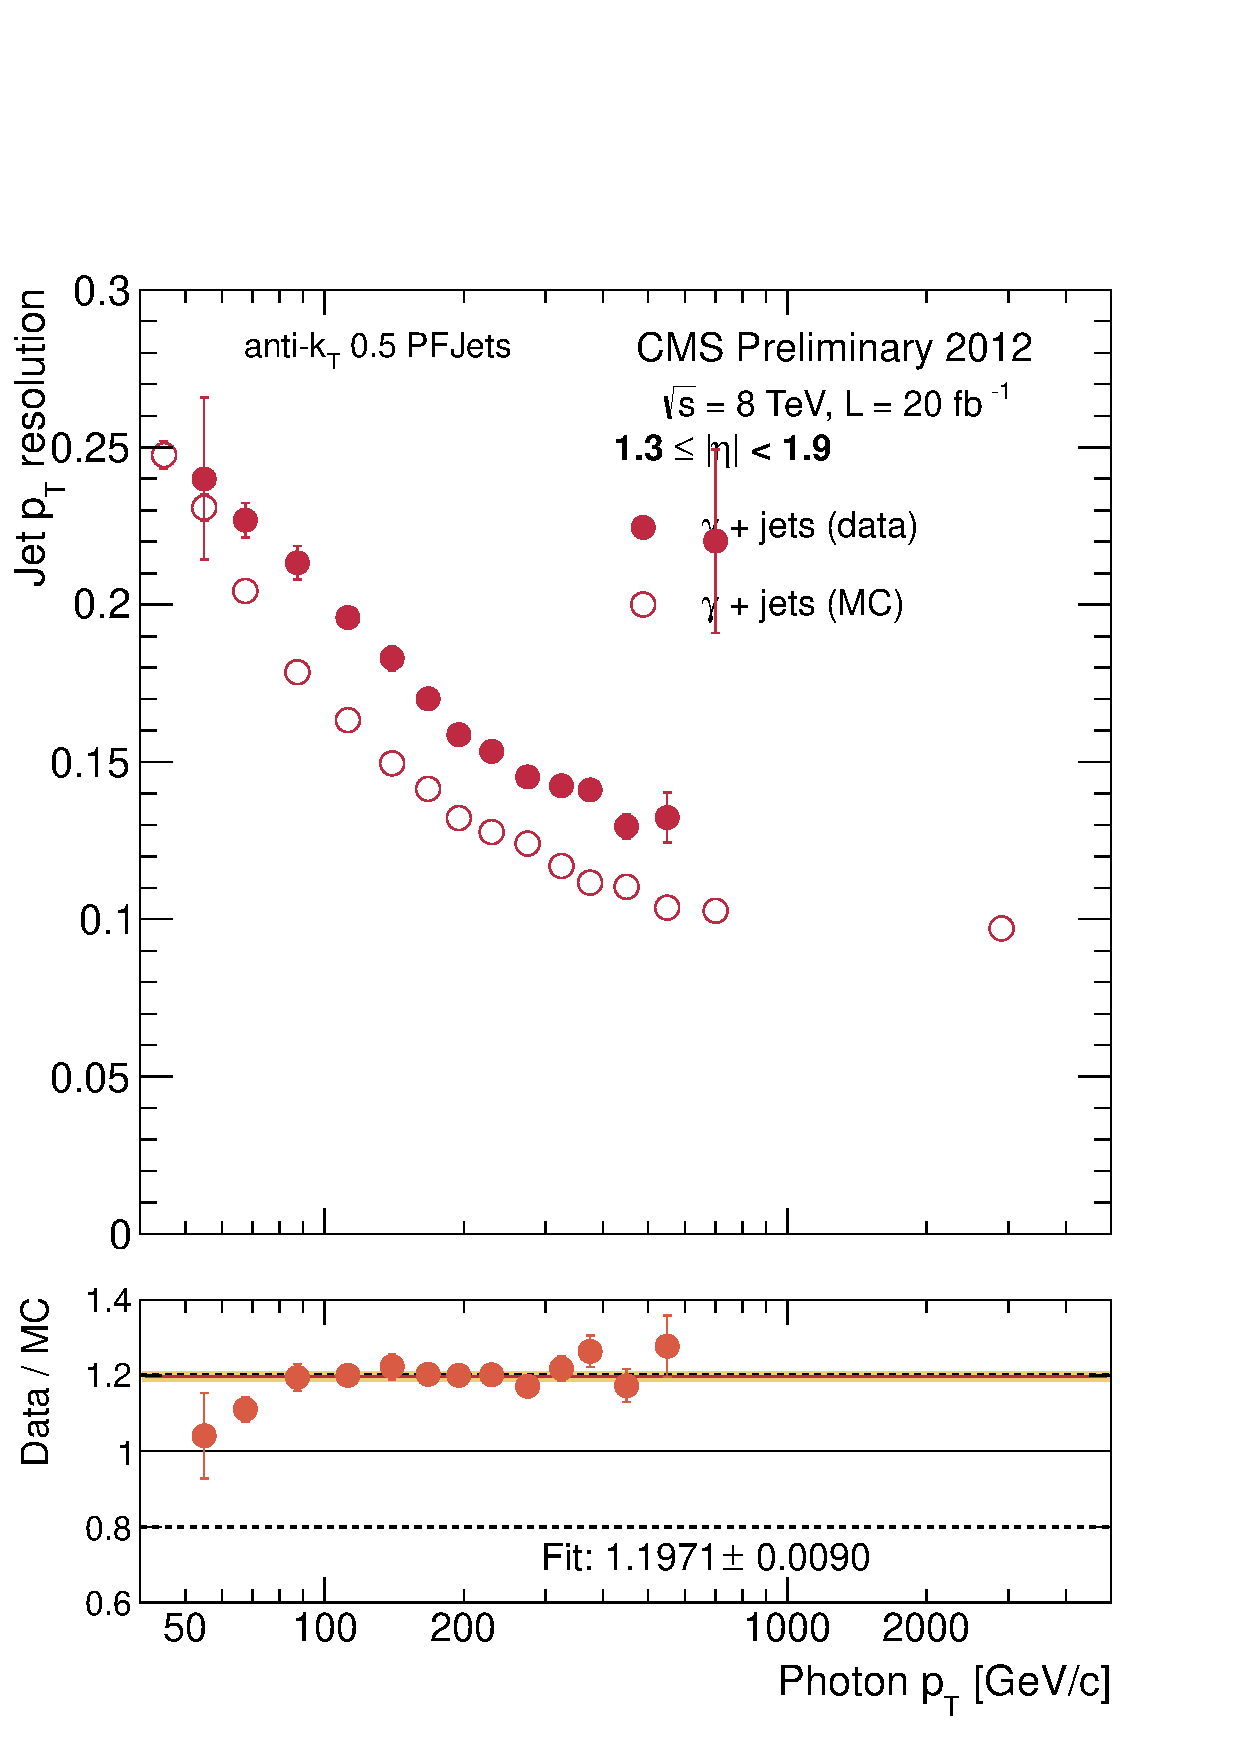
\includegraphics[width=0.45\textwidth]{chapitre4/figs/reso_balancing/resolution_eta1319_balancing.pdf}}\hfill
%     \subcaptionbox{\label{fig:reso_bal_eta1925}}[0.45\textwidth]{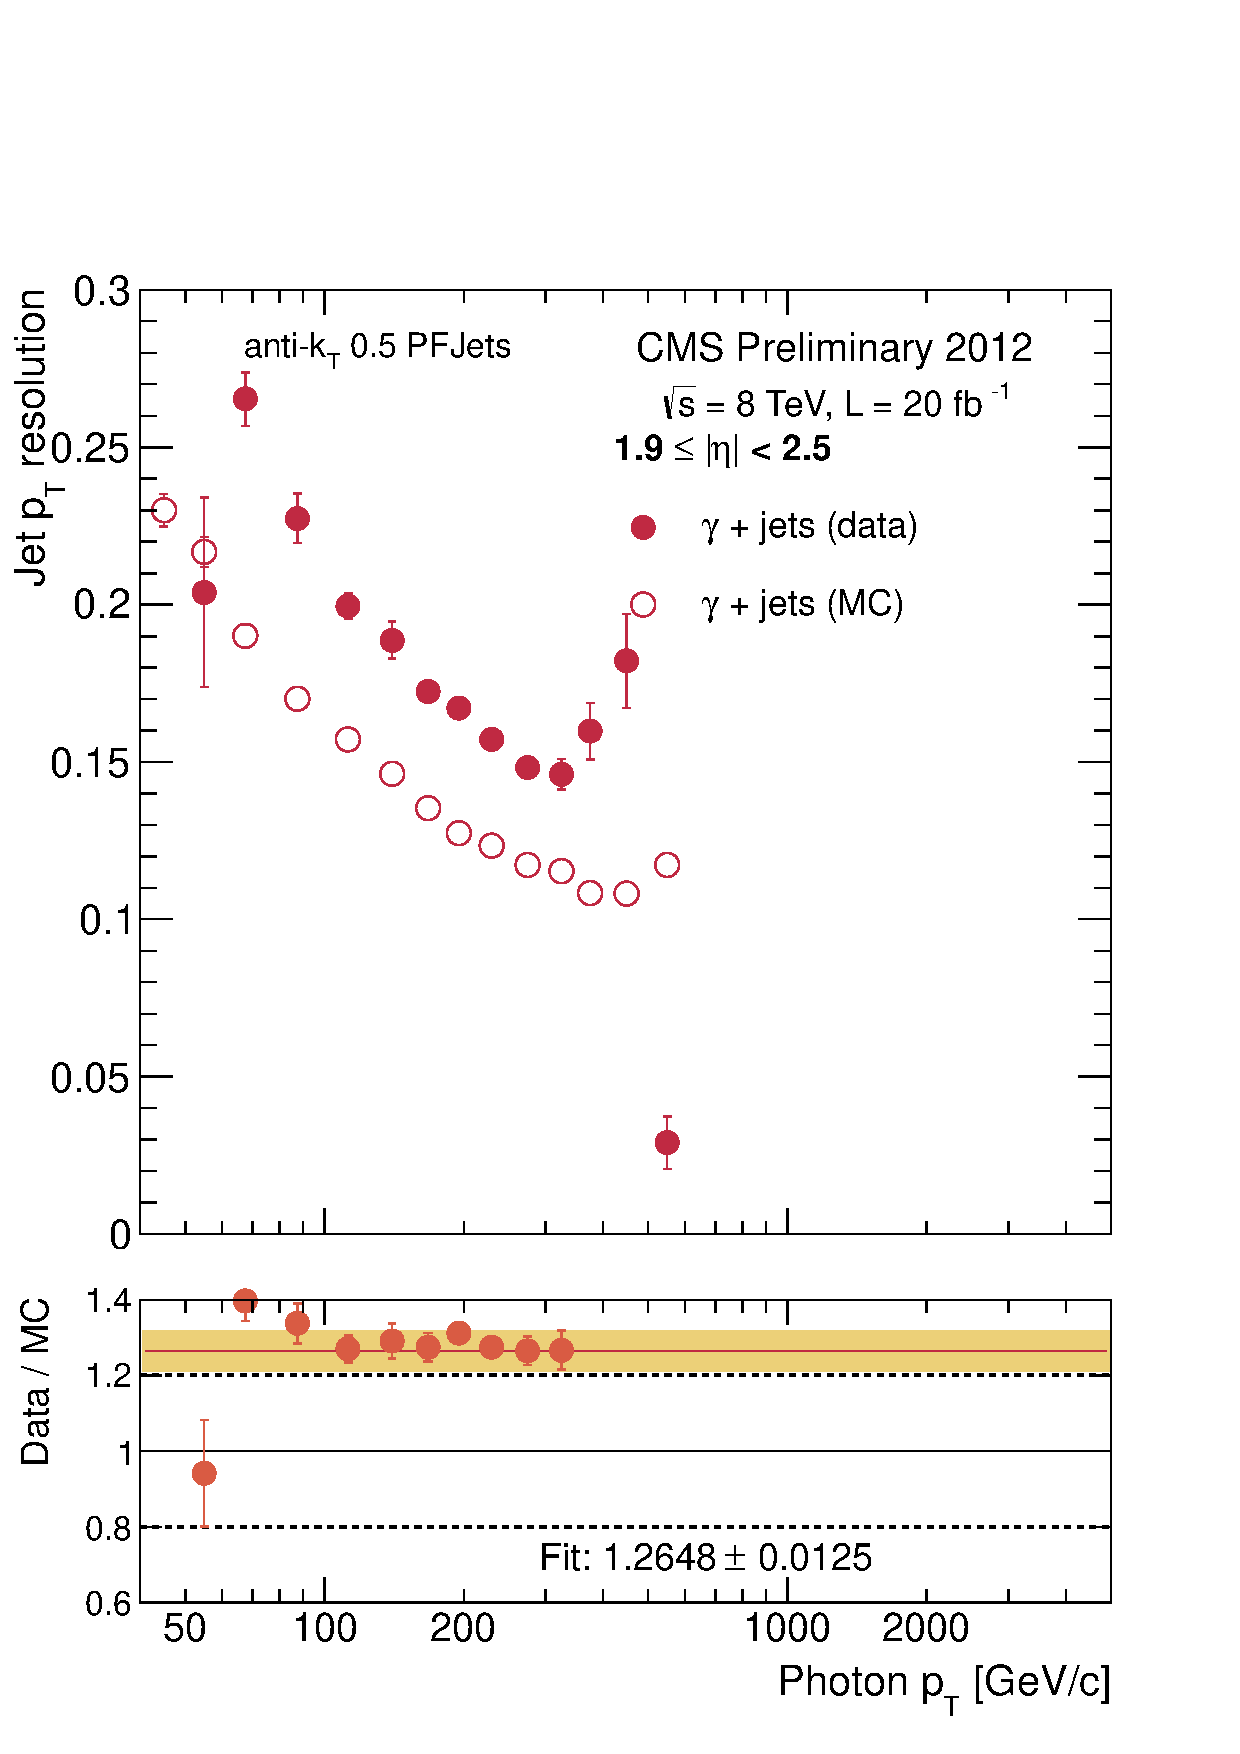
\includegraphics[width=0.45\textwidth]{chapitre4/figs/reso_balancing/resolution_eta1925_balancing.pdf}}
%     \caption{Résolutions pour la méthode de la balance pour $\aeta < \num{0.8}$ (\subref{fig:reso_bal_eta008}), $\num{0.8} \leq \aeta < \num{1.3}$ (\subref{fig:reso_bal_eta0813}), $\num{1.3} \leq \aeta < \num{1.9}$ (\subref{fig:reso_bal_eta1319}), et $\num{1.9} \leq \aeta < \num{2.5}$ (\subref{fig:reso_bal_eta1925}). Le ratio entre les données et la simulation est présenté sous chaque distribution, accompagné d'une interpolation linéaire constante (ligne orange). La bande jaune représente l'erreur sur cette interpolation.}
%     \label{fig:balancing_reso}
% \end{figure}

\begin{table}[p!] \centering
 \begin{tabular}{@{}ccc@{}} \toprule
 Classe en \aeta & ratio & $f$ \\ \midrule
 \num{0} - \num{0.8} & \num{0.966 \pm 0.001} & \num{1.035 \pm 0.001}\\
 \num{0.8} - \num{1.3} & \num{0.957 \pm 0.001} & \num{1.044 \pm 0.001}\\
 \num{1.3} - \num{1.9} & \num{0.958 \pm 0.001} & \num{1.044 \pm 0.001}\\
 \num{1.9} - \num{2.5} & \num{0.935 \pm 0.002} & \num{1.070 \pm 0.002}\\
 \num{2.5} - \num{3} & \num{0.909 \pm 0.005} & \num{1.100 \pm 0.005}\\
 \num{3} - \num{3.2} & \num{0.813 \pm 0.012} & \num{1.230 \pm 0.018}\\
 \num{3.2} - \num{5.2} & \num{0.429 \pm 0.025} & \num{2.333 \pm 0.136}\\
 \bottomrule
 \end{tabular}
 \caption{Ratios et facteurs de correction pour différentes classes en \aeta obtenus grâce à la méthode de la balance, sans extrapolation.}
 \label{tab:res_balancing}
\end{table}

\begin{table}[p!] \centering
 \begin{tabular}{@{}ccc@{}} \toprule
 Classe en \aeta & ratio & $f$ \\ \midrule
 \num{0} - \num{0.8} & \num{0.974 \pm 0.001} & \num{1.027 \pm 0.001}\\
 \num{0.8} - \num{1.3} & \num{0.966 \pm 0.001} & \num{1.036 \pm 0.001}\\
 \num{1.3} - \num{1.9} & \num{0.961 \pm 0.001} & \num{1.041 \pm 0.001}\\
 \num{1.9} - \num{2.5} & \num{0.944 \pm 0.002} & \num{1.060 \pm 0.002}\\
 \num{2.5} - \num{3} & \num{0.923 \pm 0.005} & \num{1.083 \pm 0.006}\\
 \num{3} - \num{3.2} & \num{0.844 \pm 0.013} & \num{1.185 \pm 0.018}\\
 \num{3.2} - \num{5.2} & -  & -\\
 \bottomrule
 \end{tabular}
 \caption{Ratios et facteurs de correction pour différentes classes en \aeta obtenus grâce à la méthode de la balance, avec extrapolation.}
 \label{tab:res_balancing_extrap}
\end{table}


\begin{figure}[p!]
    \centering
    \subcaptionbox{\label{fig:bal_extrap_eta008}}[0.45\textwidth]{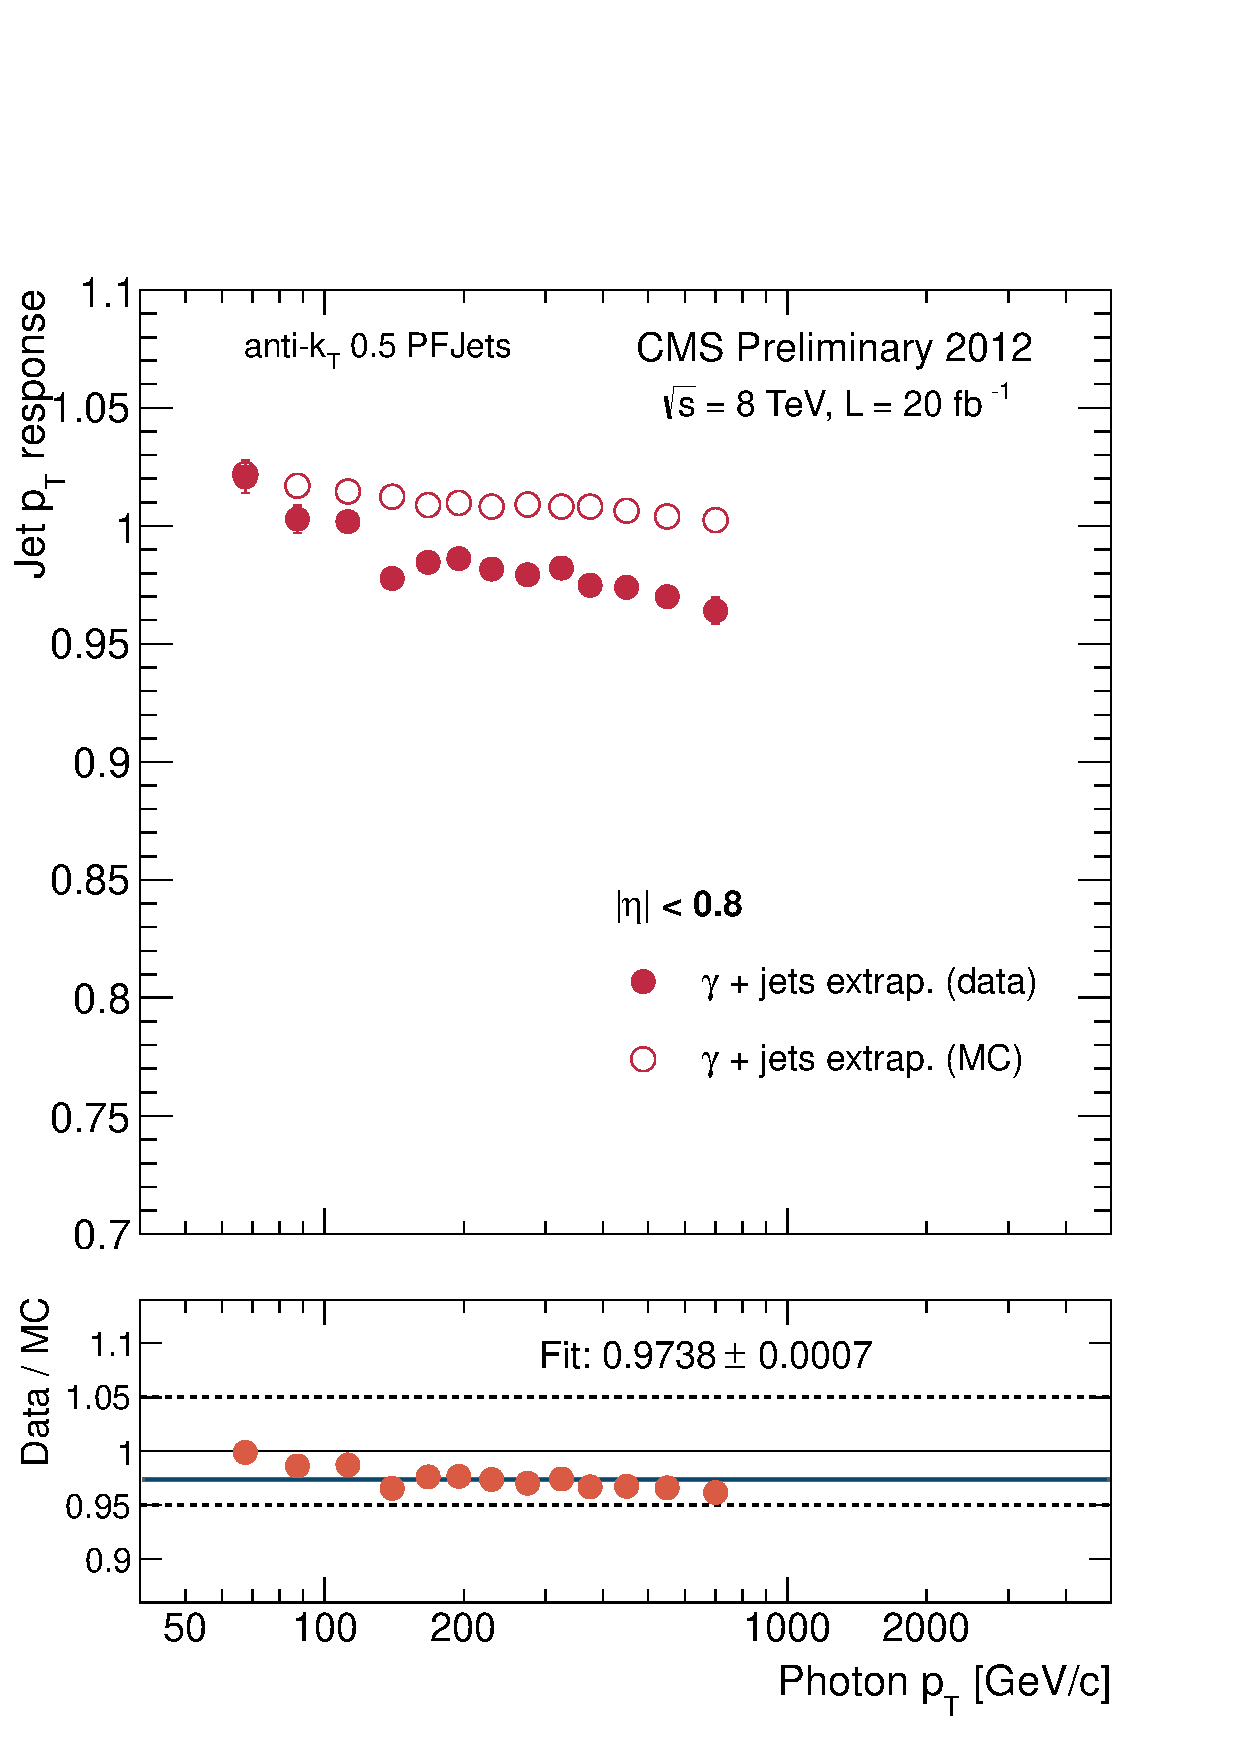
\includegraphics[width=0.45\textwidth]{chapitre4/figs/resp_balancing_extrap/response_eta008_balancing_extrap.pdf}}\hfill
    \subcaptionbox{\label{fig:bal_extrap_eta0813}}[0.45\textwidth]{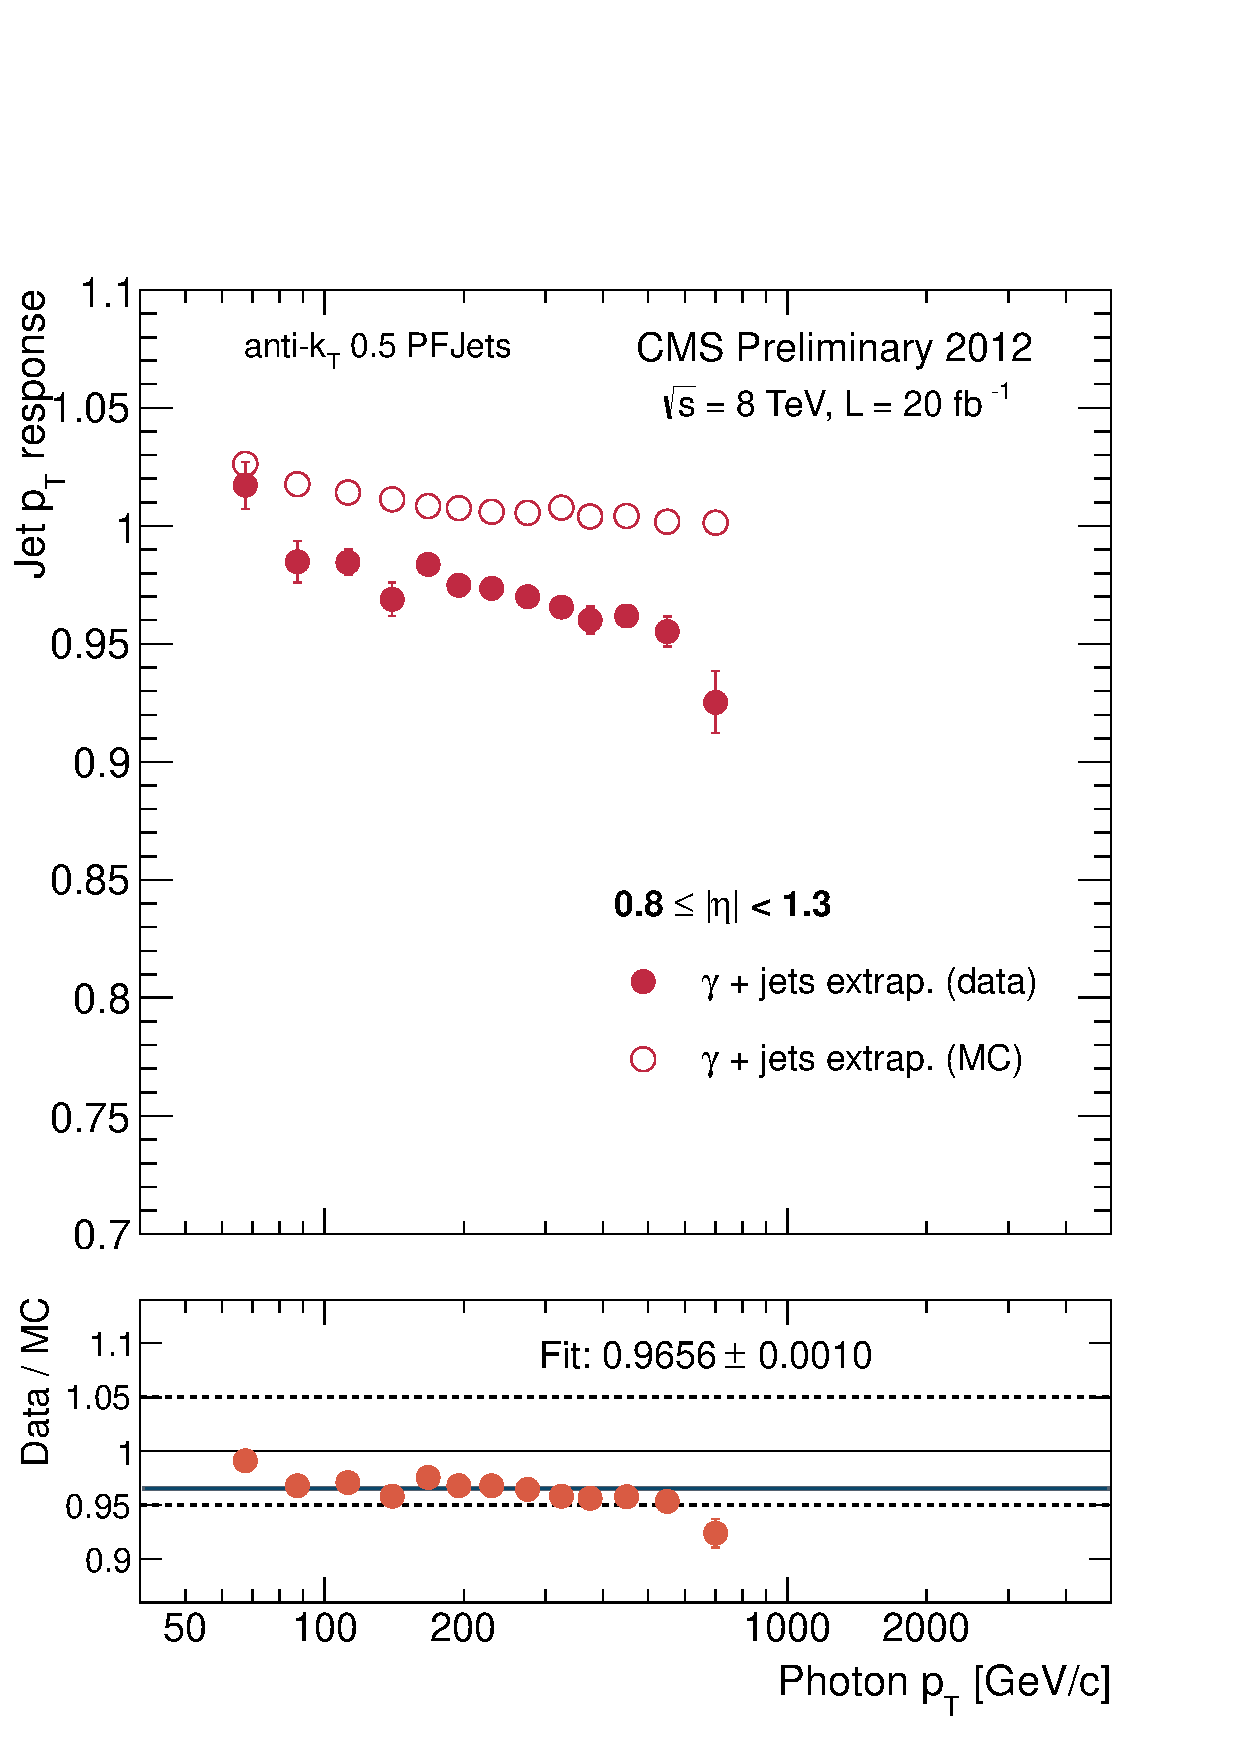
\includegraphics[width=0.45\textwidth]{chapitre4/figs/resp_balancing_extrap/response_eta0813_balancing_extrap.pdf}}
    \subcaptionbox{\label{fig:bal_extrap_eta1319}}[0.45\textwidth]{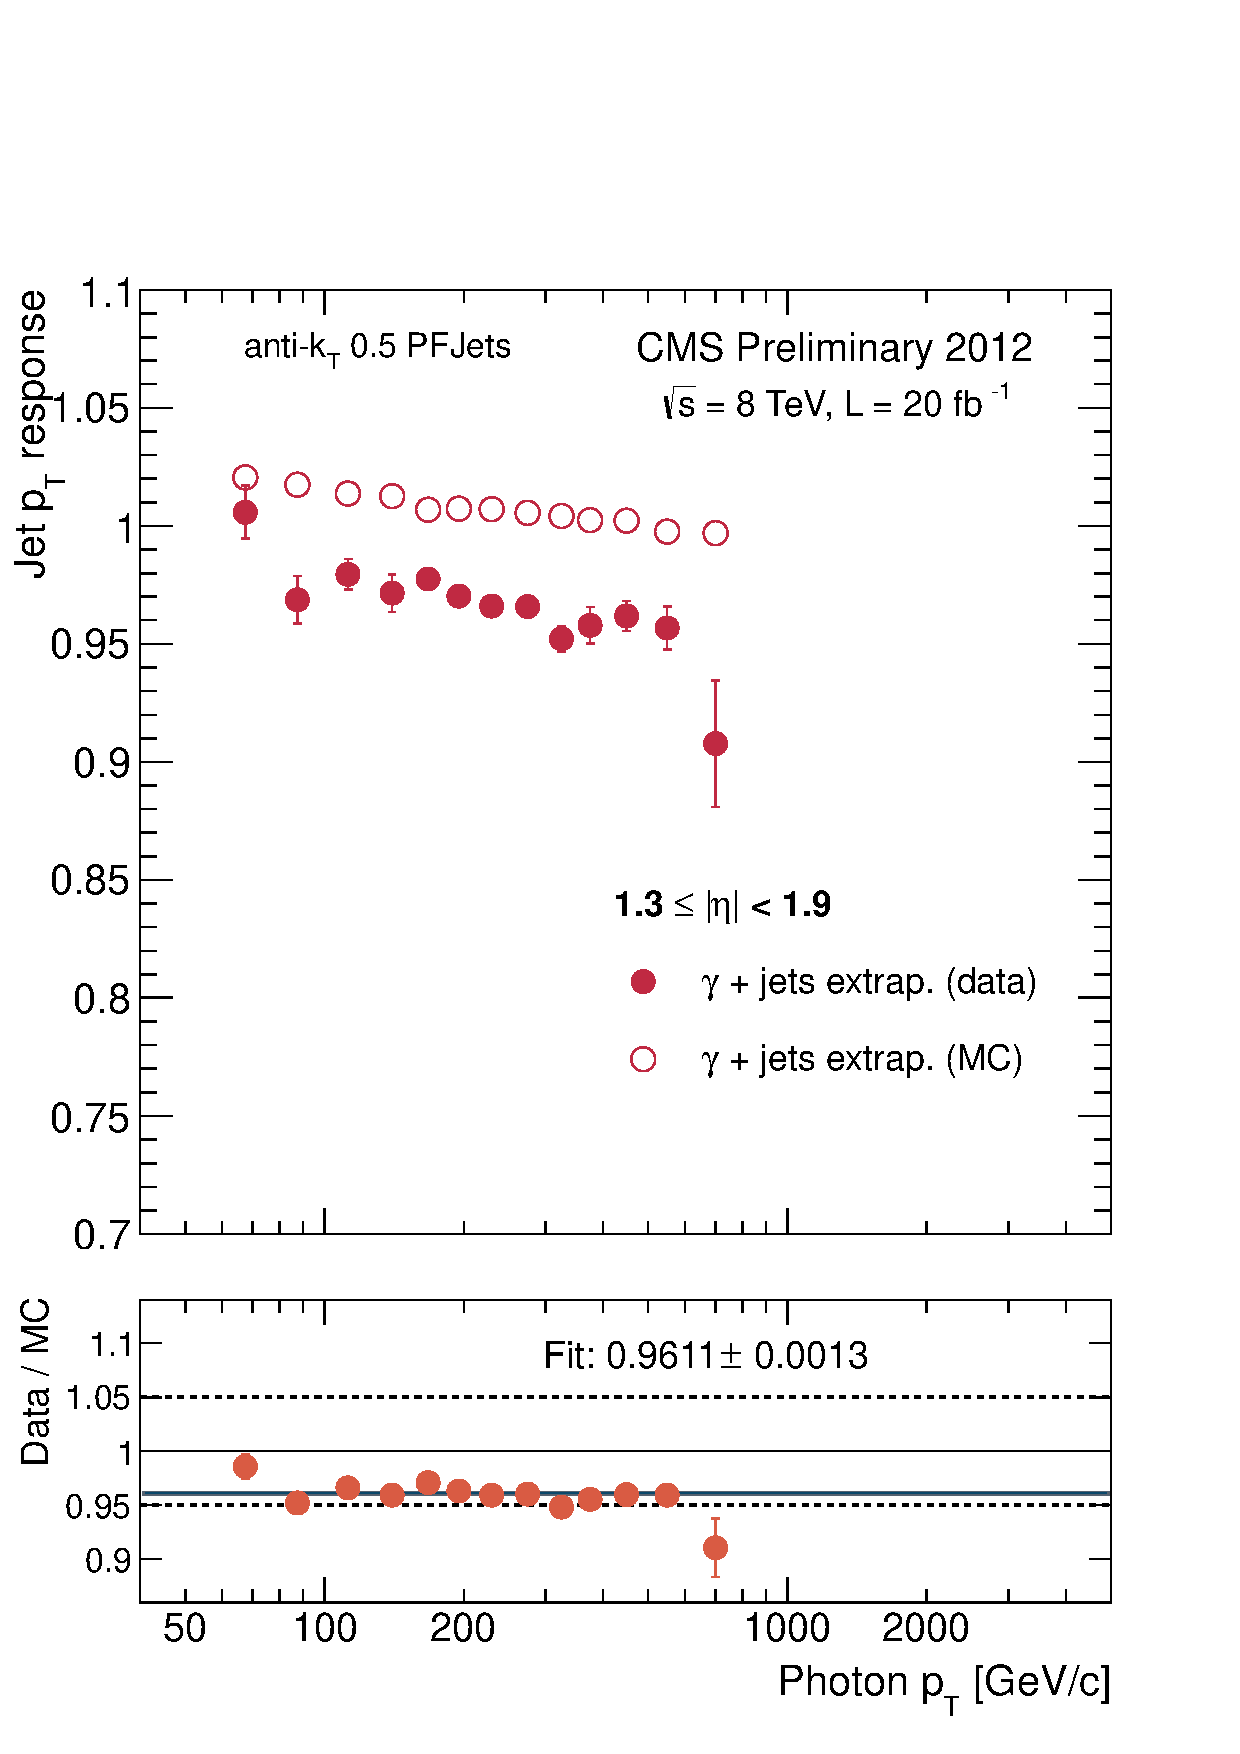
\includegraphics[width=0.45\textwidth]{chapitre4/figs/resp_balancing_extrap/response_eta1319_balancing_extrap.pdf}}\hfill
    \subcaptionbox{\label{fig:bal_extrap_eta1925}}[0.45\textwidth]{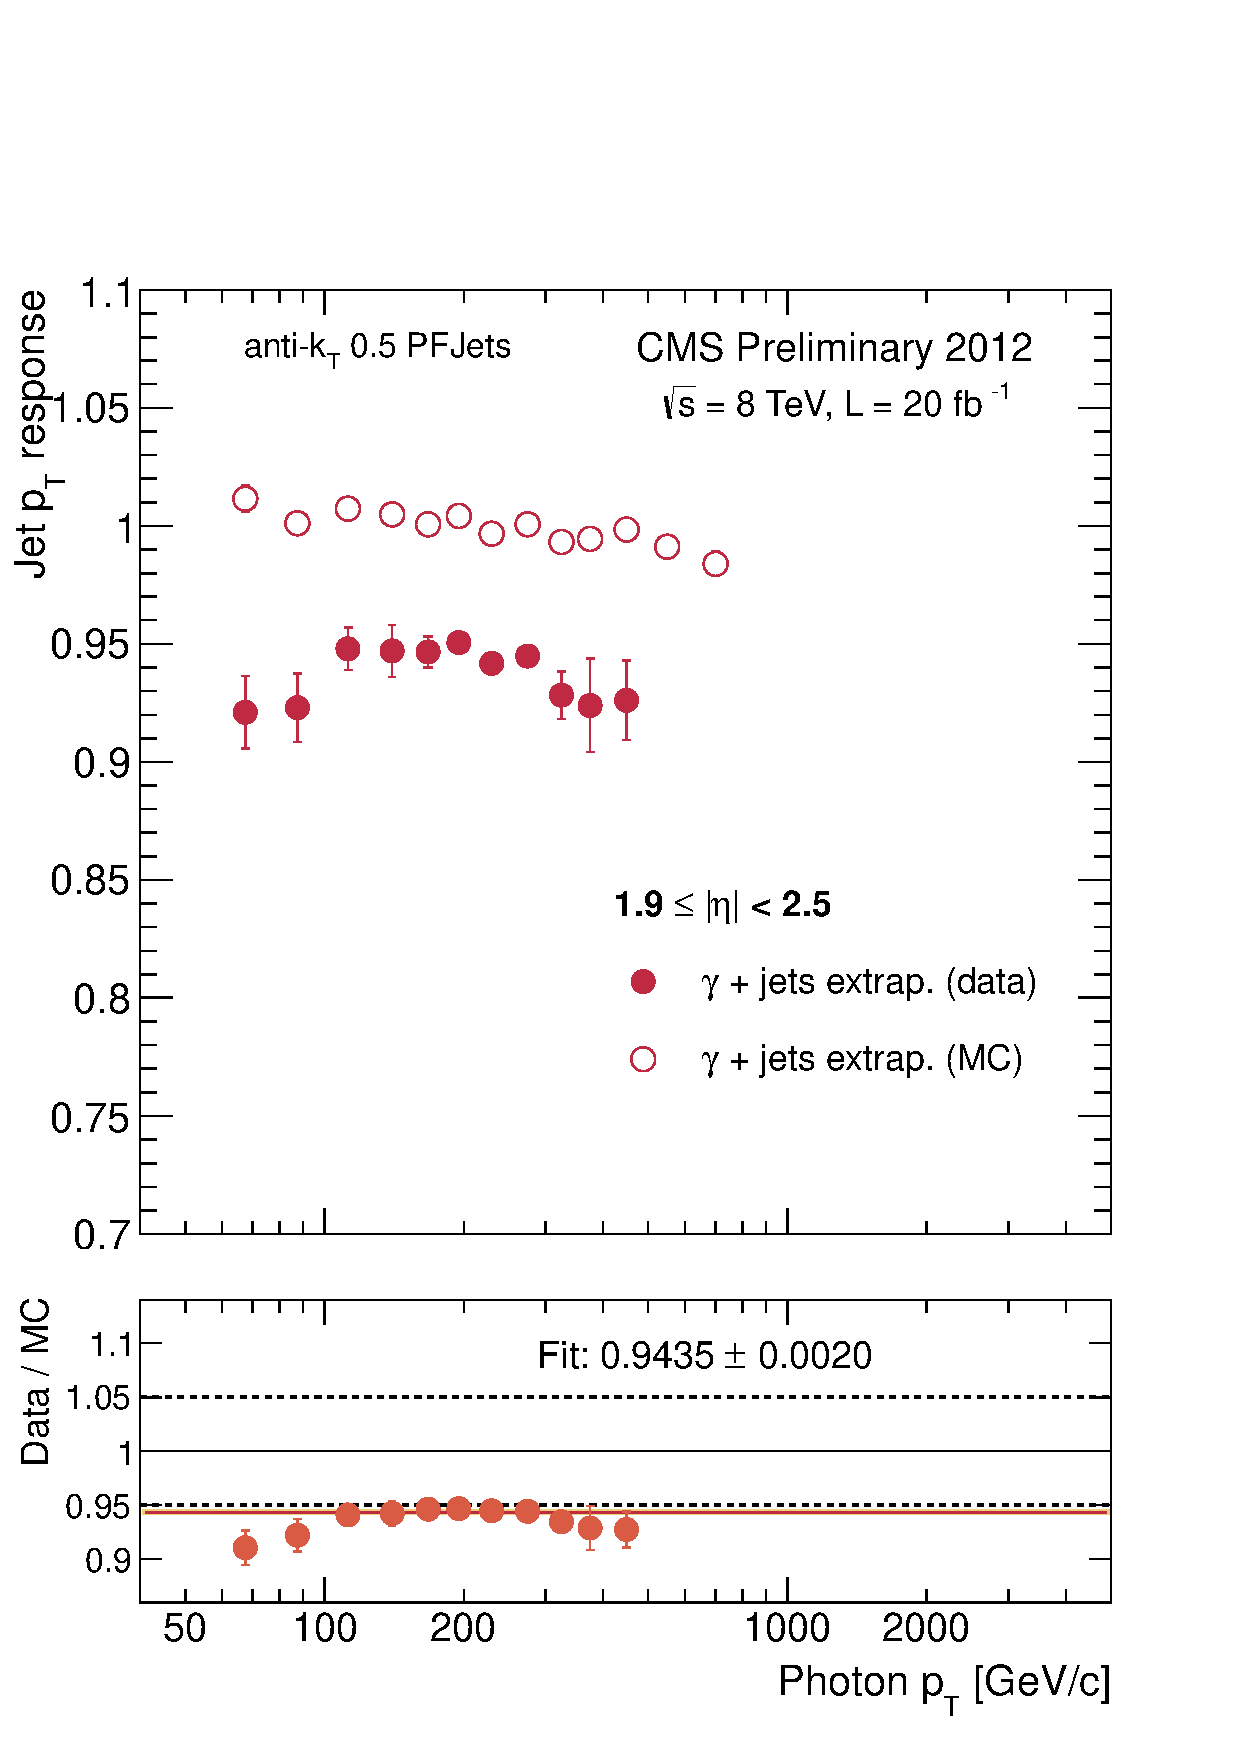
\includegraphics[width=0.45\textwidth]{chapitre4/figs/resp_balancing_extrap/response_eta1925_balancing_extrap.pdf}}
    \caption{Réponses moyennes pour la méthode de la balance, avec extrapolation, pour $\aeta < \num{0.8}$ (\subref{fig:bal_extrap_eta008}), $\num{0.8} \leq \aeta < \num{1.3}$ (\subref{fig:bal_extrap_eta0813}), $\num{1.3} \leq \aeta < \num{1.9}$ (\subref{fig:bal_extrap_eta1319}), et $\num{1.9} \leq \aeta < \num{2.5}$ (\subref{fig:bal_extrap_eta1925}). Le ratio entre les données et la simulation est présenté sous chaque distribution, accompagné d'une interpolation linéaire constante (ligne orange). La bande jaune représente l'erreur sur cette interpolation.}
    \label{fig:balancing_extrap_resp}
\end{figure}

\bigskip

On présente dans le \cref{tab:res_balancing} un résumé des ratios et des facteurs de correction extrais pour chaque classe en \aeta. Le ratio est stable dans le tonneau ($\aeta < \num{2.1}$), avec un facteur de correction d'environ \SI{4}{\%}. Dans les bouchons, le ratio chute jusqu'à des facteurs de correction atteignant \SI{23}{\%}. Au delà de \SI{3.2}{\radian}, l'absence de trajectographe empêche la bonne reconstruction des hadrons chargés, et la réponse devient très mauvaise.

\subsubsection{Dépendance de la réponse en fonction de l'activité additionnelle} \label{sec:res_balancing_extrap}

\begin{figure}[tbp]
    \centering
    \subcaptionbox{\label{fig:extrap_balancing}}[0.45\textwidth]{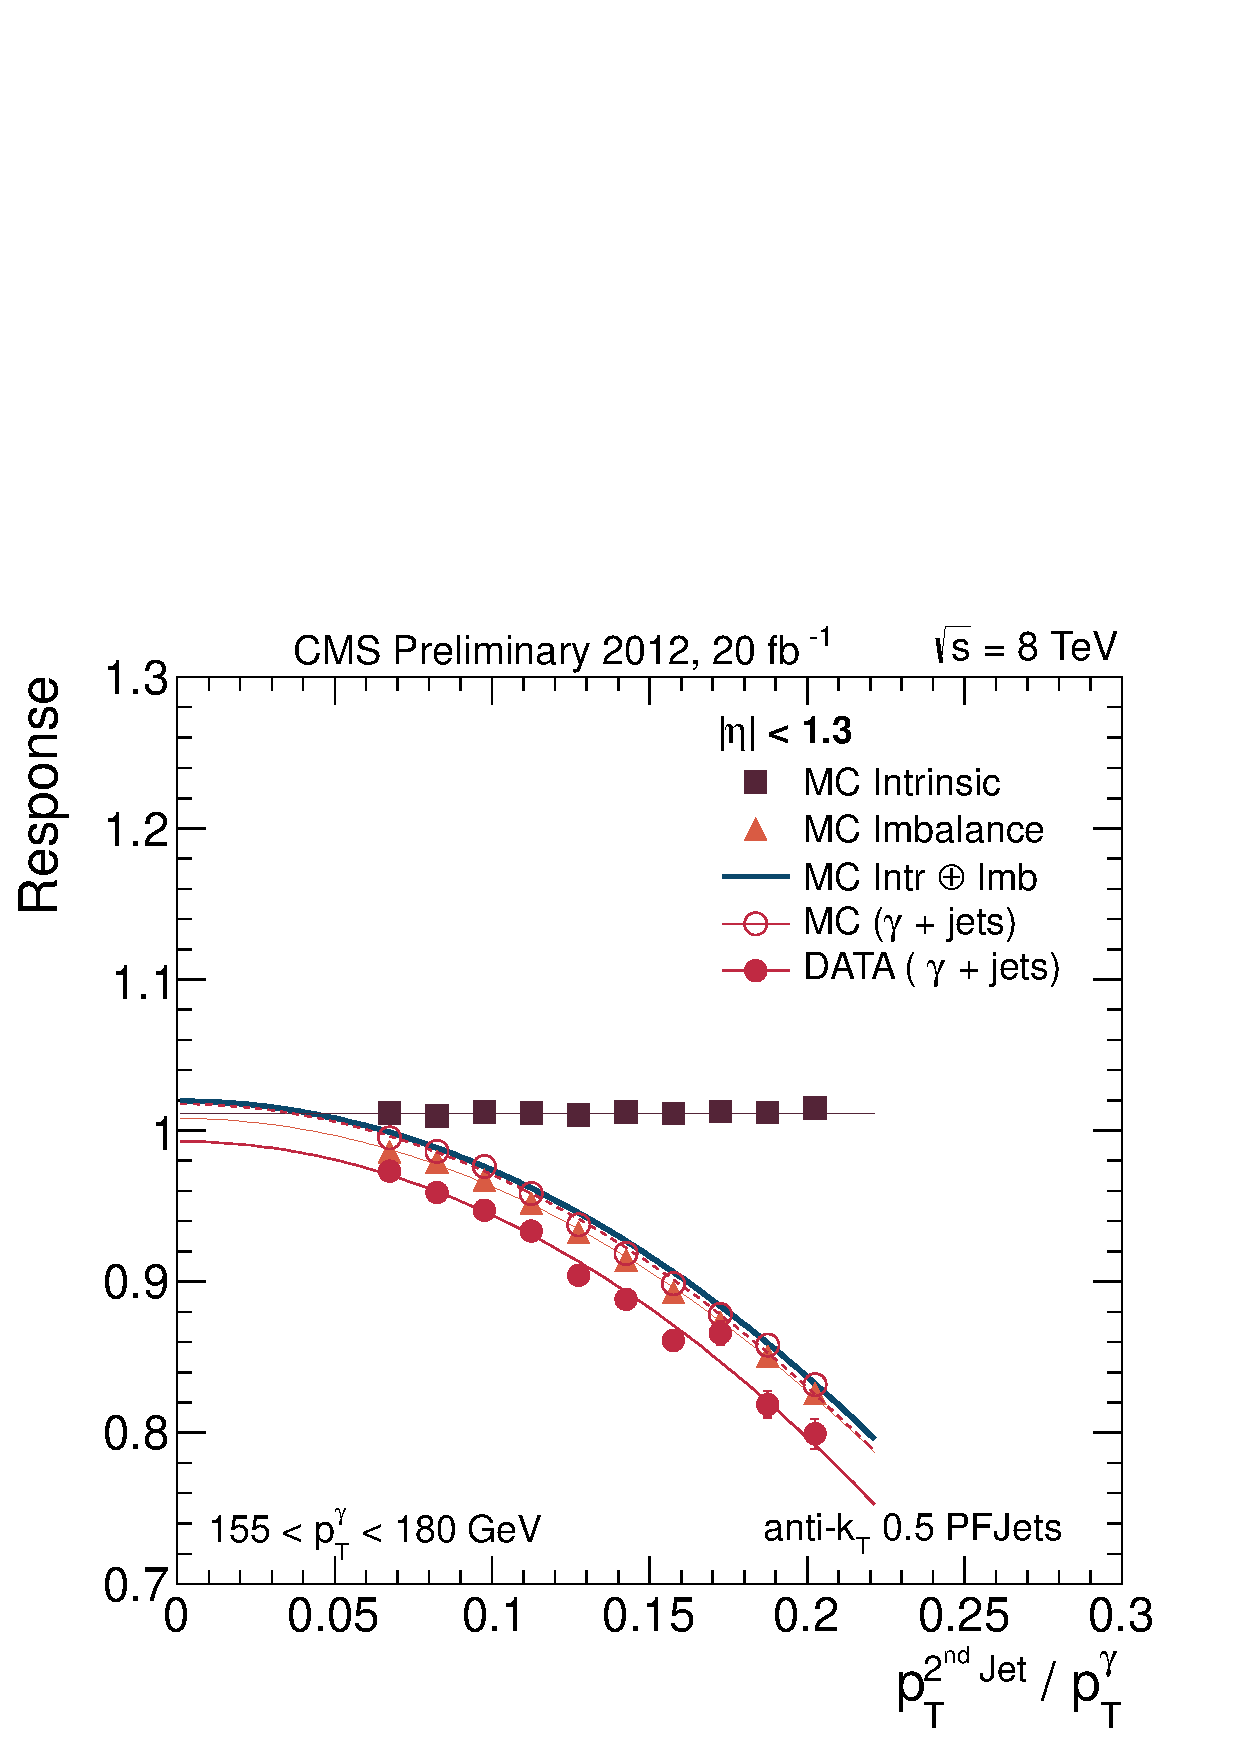
\includegraphics[width=0.45\textwidth]{chapitre4/figs/extrap/response_eta013_ptPhot_155_180.pdf}}\hfill
    \subcaptionbox{\label{fig:extrap_mpf}}[0.45\textwidth]{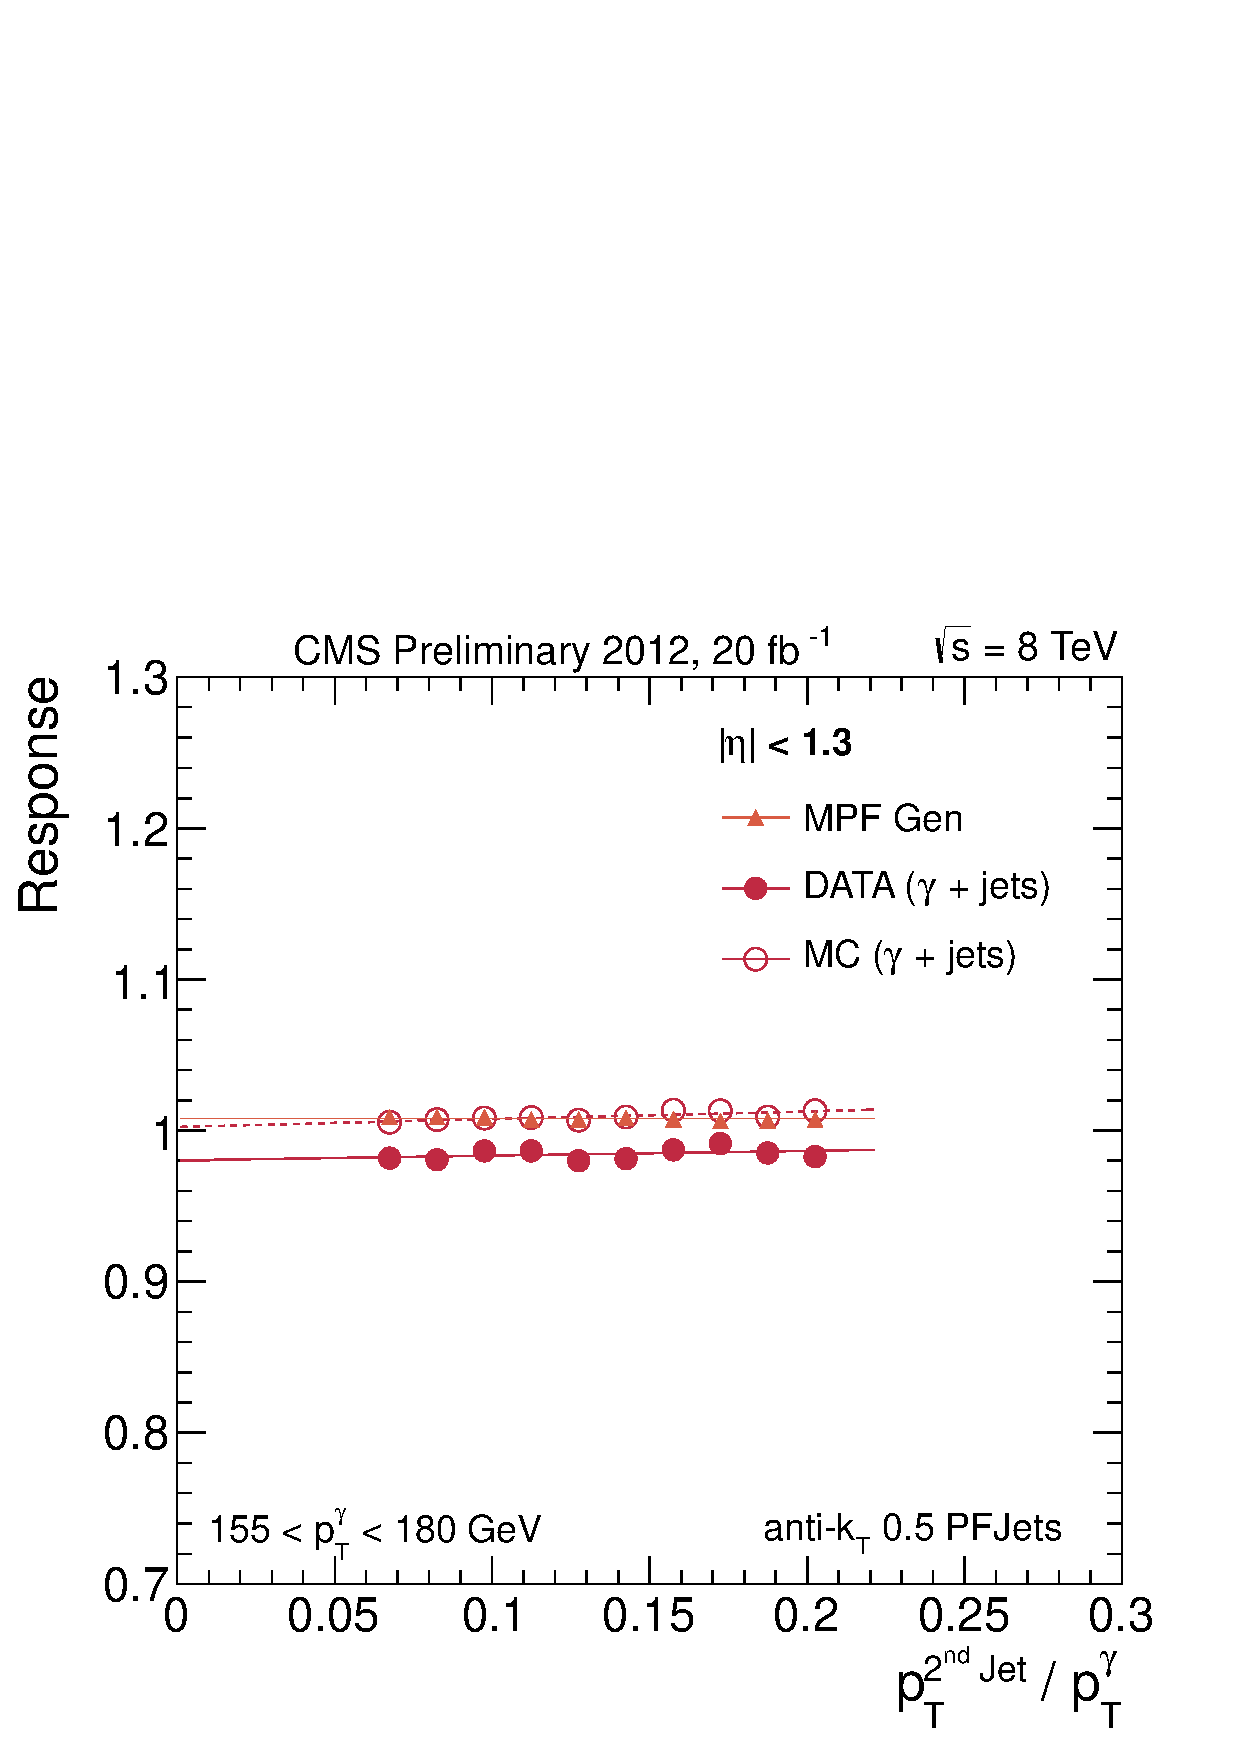
\includegraphics[width=0.45\textwidth]{chapitre4/figs/extrap/responseMPF_eta013_ptPhot_155_180.pdf}}
    \caption{Extrapolation de la réponse moyenne pour la méthode de la balance (\subref{fig:extrap_balancing}) et la méthode MPF (\subref{fig:extrap_mpf}). Pour la méthode de la balance, la réponse de la simulation (MC) a été séparée en deux parties, détaillées \cref{sec:res_balancing_extrap}.}
\end{figure}


% \begin{figure}[p!]
%     \centering
%     \subcaptionbox{\label{fig:reso_bal_extrap_eta008}}[0.45\textwidth]{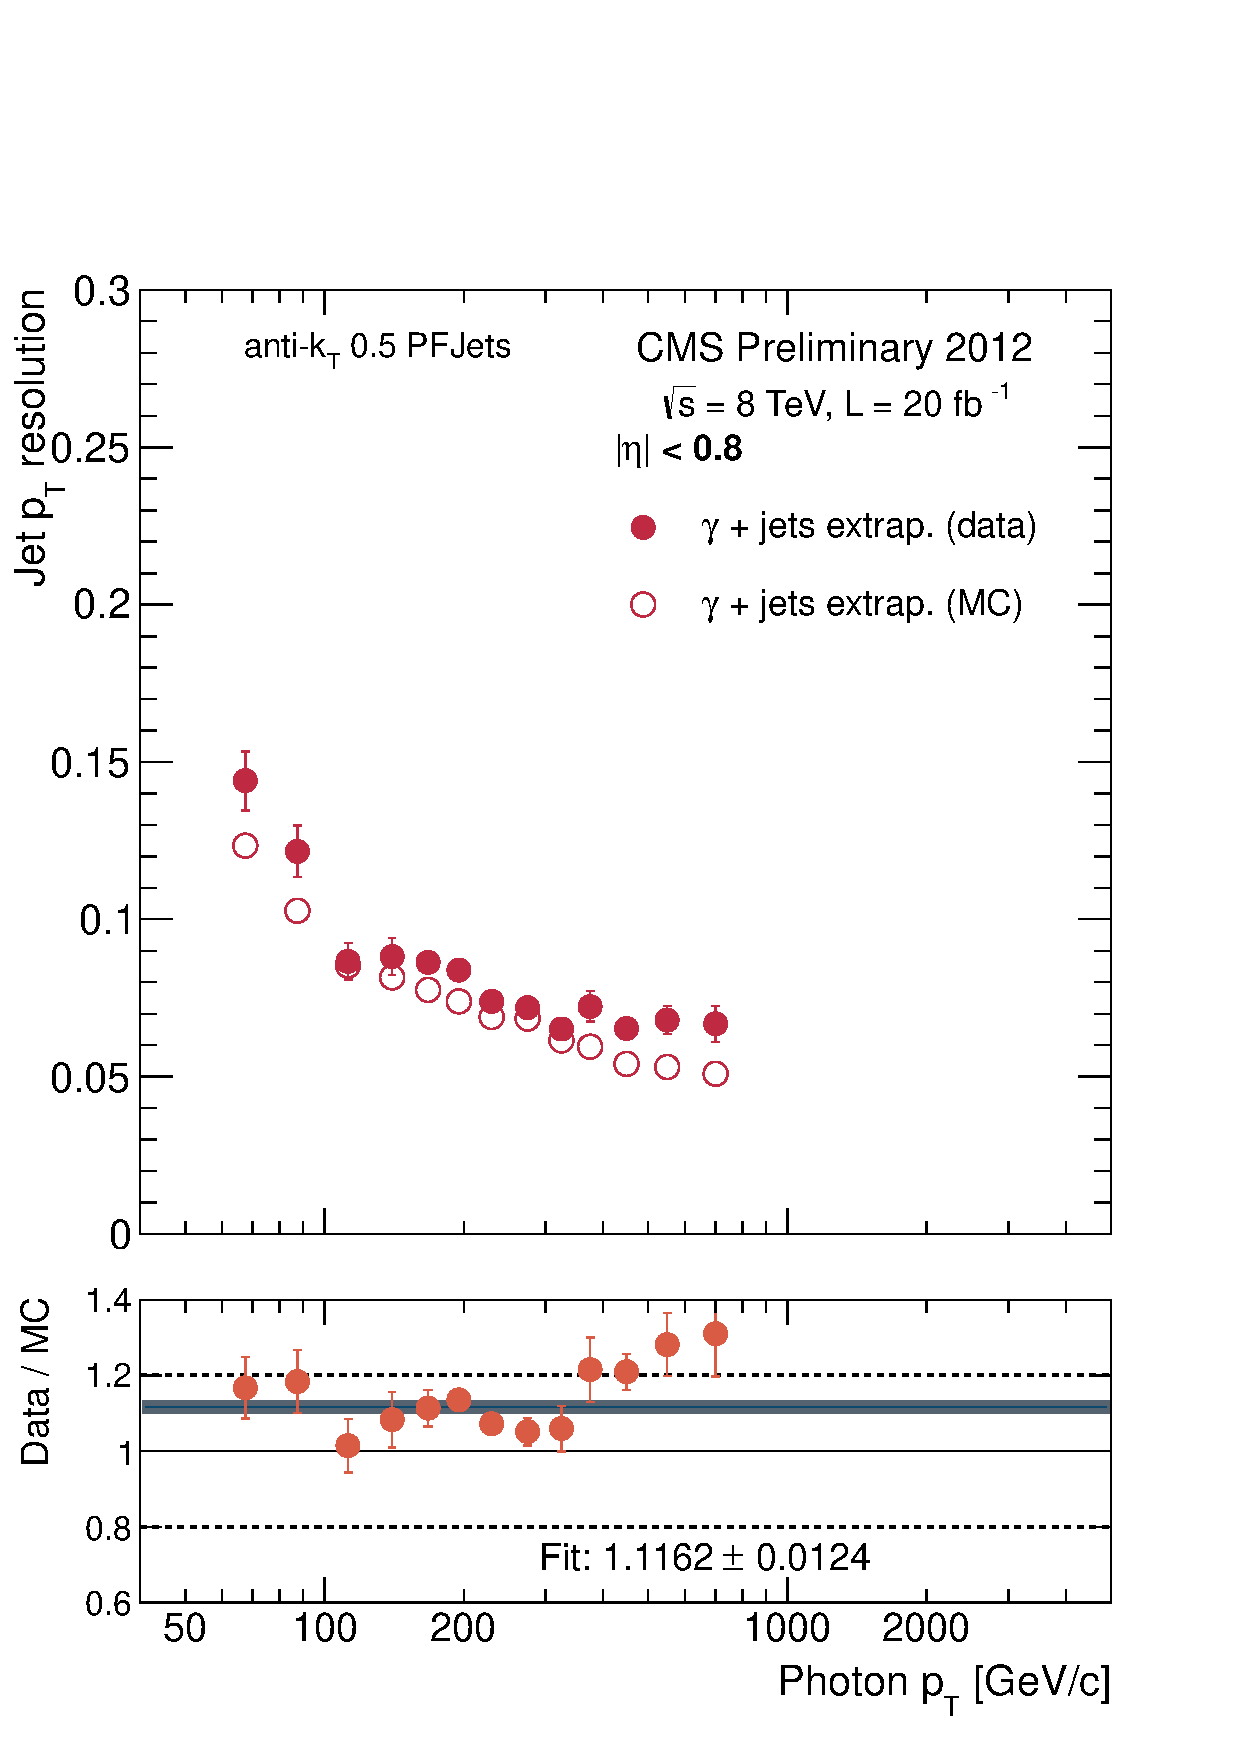
\includegraphics[width=0.45\textwidth]{chapitre4/figs/reso_balancing_extrap/resolution_eta008_balancing_extrap.pdf}}\hfill
%     \subcaptionbox{\label{fig:reso_bal_extrap_eta0813}}[0.45\textwidth]{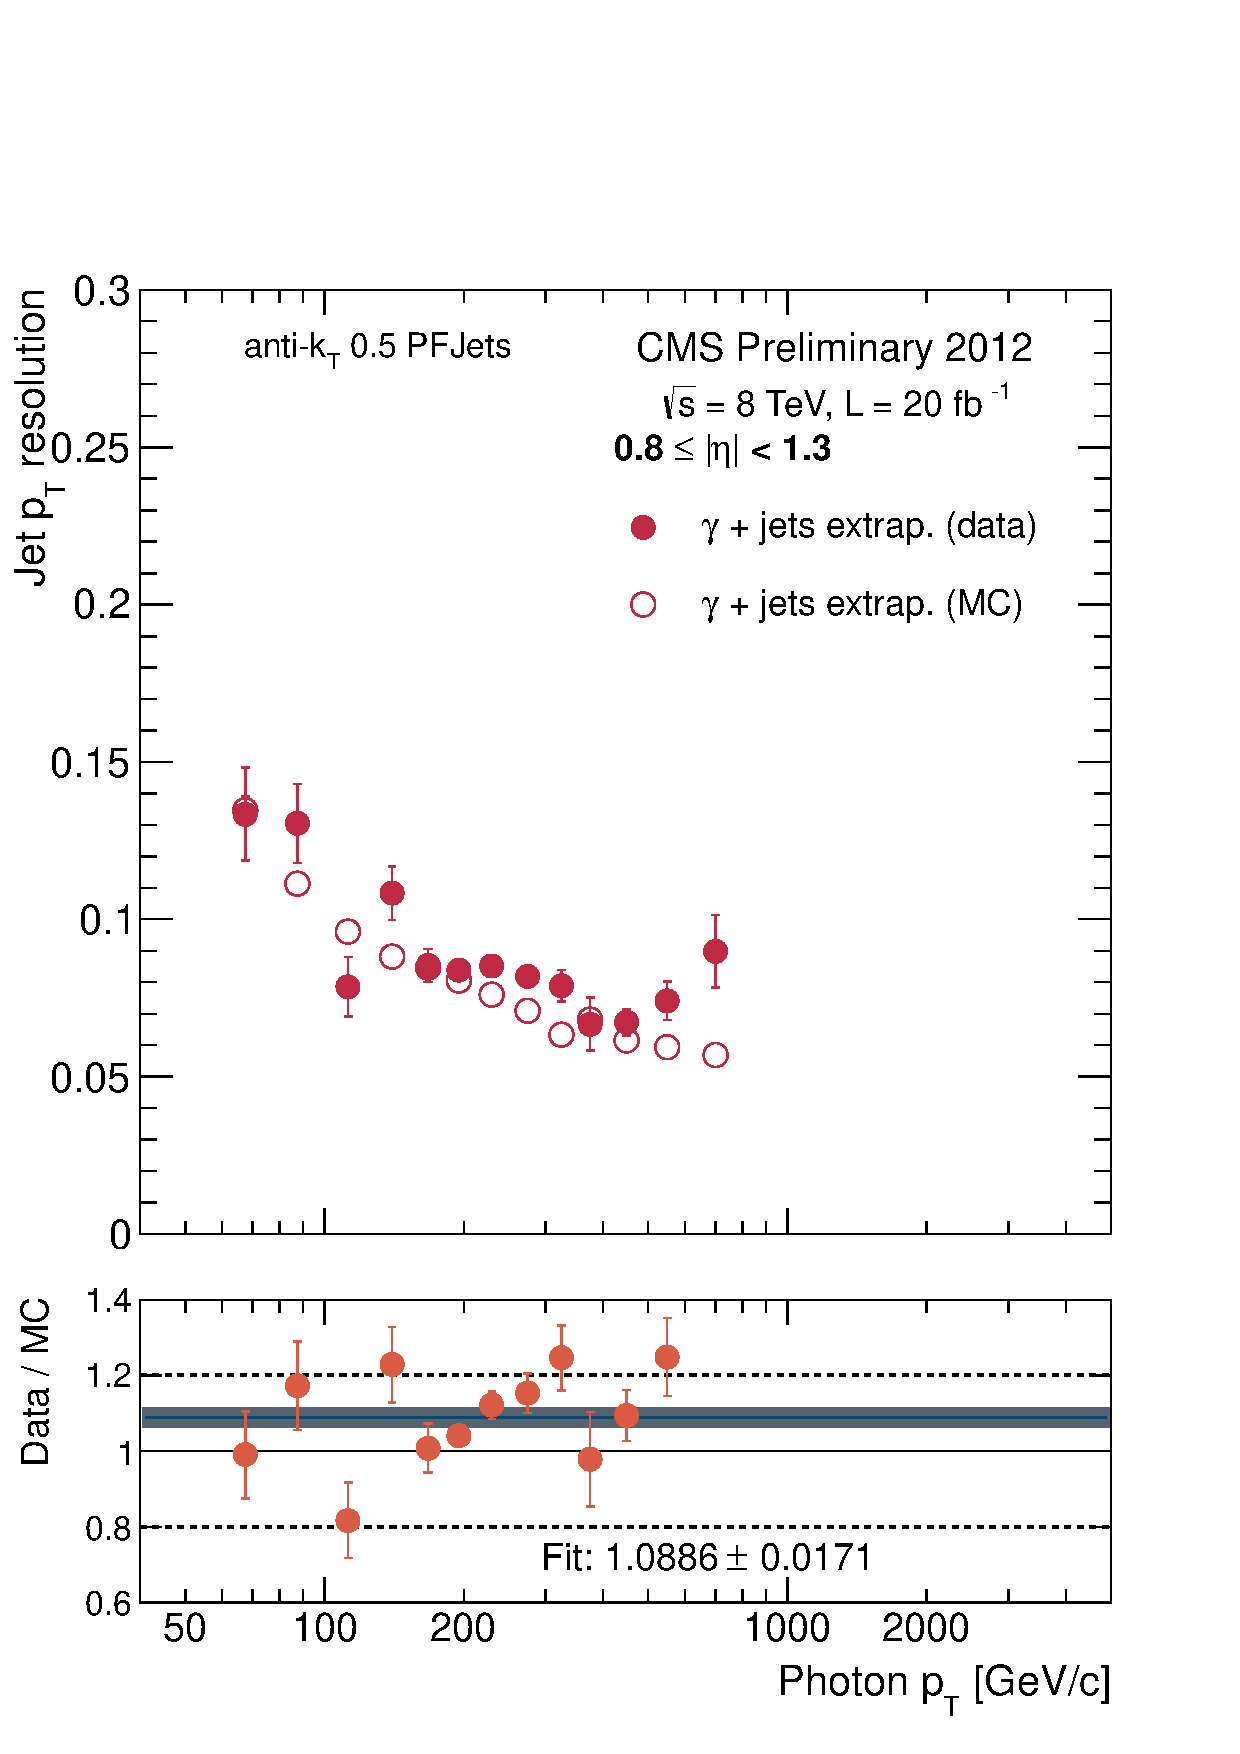
\includegraphics[width=0.45\textwidth]{chapitre4/figs/reso_balancing_extrap/resolution_eta0813_balancing_extrap.pdf}}
%     \subcaptionbox{\label{fig:reso_bal_extrap_eta1319}}[0.45\textwidth]{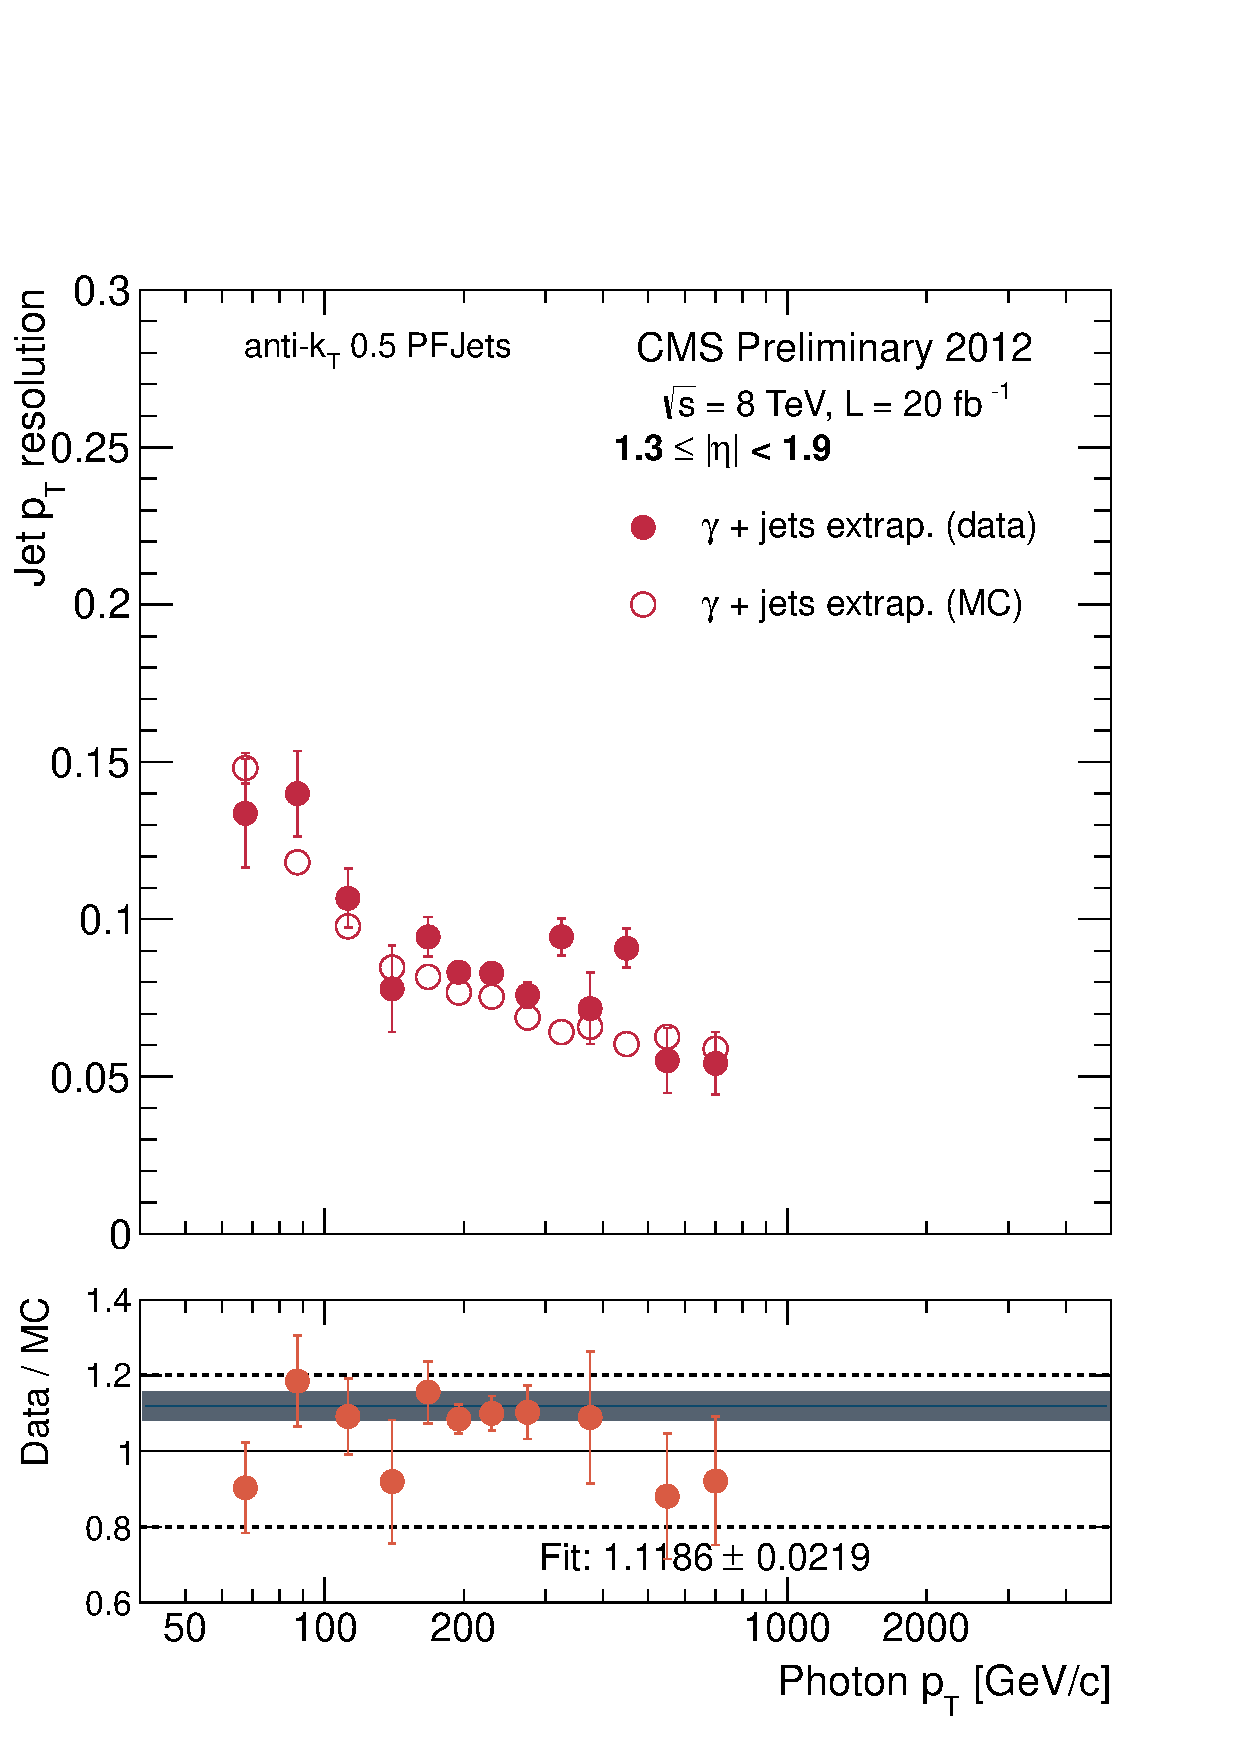
\includegraphics[width=0.45\textwidth]{chapitre4/figs/reso_balancing_extrap/resolution_eta1319_balancing_extrap.pdf}}\hfill
%     \subcaptionbox{\label{fig:reso_bal_extrap_eta1925}}[0.45\textwidth]{\includegraphics[width=0.45\textwidth]{chapitre4/figs/reso_balancing_extrap/resolution_eta1925_balancing_extrap.pdf}}
%     \caption{Résolutions pour la méthode de la balance, avec extrapolation, pour $\aeta < \num{0.8}$ (\subref{fig:reso_bal_extrap_eta008}), $\num{0.8} \leq \aeta < \num{1.3}$ (\subref{fig:reso_bal_extrap_eta0813}), $\num{1.3} \leq \aeta < \num{1.9}$ (\subref{fig:reso_bal_extrap_eta1319}), et $\num{1.9} \leq \aeta < \num{2.5}$ (\subref{fig:reso_bal_extrap_eta1925}). Le ratio entre les données et la simulation est présenté sous chaque distribution, accompagné d'une interpolation linéaire constante (ligne orange). La bande jaune représente l'erreur sur cette interpolation.}
%     \label{fig:balancing_extrap_reso}
% \end{figure}

On a vu précédemment que la méthode de la balance était sensible à la présence de jets additionnels dans l'événement. Afin de corriger cet effet, on extrapole la réponse moyenne à $\alpha \rightarrow 0$. On présente \cref{fig:extrap_balancing} un exemple d'extrapolation pour la méthode de la balance, pour $155 \leq p_T^\gamma < \SI{180}{\GeV}$ et $\aeta < \num{1.3}$, et \cref{fig:extrap_mpf} pour la méthode MPF. On constate une très nette dépendance de la réponse moyenne en fonction de $\alpha$ pour la méthode de la balance. Au contraire, la méthode MPF n'est pas dépendante de la présence d'activité additionnelle. Ce comportement est attendu puisque, par définition, la méthode MPF utilise déjà l'activité additionnelle pour calculer la réponse ($p_T^\text{recul}$, voir \cref{sec:mpf}).

Pour la méthode de la balance, on sépare la réponse de la simulation en deux parties. On a
\begin{align*}
  R_m &= \frac{\ptfjet}{\ptg} = \underbrace{ \frac{\ptfjet}{p_T^{\text{\ordinalnum{1} jet généré}}} }_{\text{intrinsèque}} \; \times \; \underbrace{ \frac{p_T^{\text{\ordinalnum{1} jet généré}}}{\ptg} }_{\text{déséquilibre}}
\end{align*}

%\afterpage{\clearpage}

La partie intrinsèque n'est pas dépendante de la présence de jets additionnels, d'où l'allure plate \cref{fig:extrap_balancing}. Elle est uniquement sensible aux problèmes de calibrations des divers détecteurs, problèmes résolus à l'aide des corrections de niveau 1, 2 et 3. C'est ainsi qu'on obtient une réponse intrinsèque très proche de l'unité. La deuxième partie correspond au déséquilibre entre le photon et le premier jet de l'événement, et dépend fortement de $\alpha$.

On utilise comme réponse moyenne la valeur de l'interpolation pour $\alpha = 0$, et on reproduit la même procédure que section précédente. À haut \pt et haut \aeta, la statistique n'est parfois pas suffisante pour réaliser l'extrapolation. Dans ce cas, le point est simplement ignoré et n'apparaît pas dans la distribution des réponses.

On présente \cref{fig:balancing_extrap_resp} les distributions des réponses moyennes après extrapolation pour différentes classes en \aeta. Les facteurs de correction sont récapitulés dans le \cref{tab:res_balancing_extrap}. On constate une légère amélioration des ratios pour toutes les classes en \aeta. Aucun résultat n'est disponible pour la dernière classe en \aeta, le nombre d'événements n'étant pas suffisant pour effectuer une extrapolation.

\subsubsection{Méthode MPF}

On présente les distributions des réponses moyennes obtenues avec la méthode MPF \cref{fig:mpf_resp}. Un récapitulatif des résultats peut être trouvé dans le \cref{tab:res_mpf}.

\begin{table}[htb] \centering
 \begin{tabular}{@{}ccc@{}} \toprule
 Classe en \aeta & ratio & $f$ \\ \midrule
 \num{0} - \num{0.8} & \num{0.9748 \pm 0.0009} & \num{1.0258 \pm 0.0010} \\
 \num{0.8} - \num{1.3} & \num{0.9673 \pm 0.0011} & \num{1.0338 \pm 0.0012} \\
 \num{1.3} - \num{1.9} & \num{0.9649 \pm 0.0012} & \num{1.0364 \pm 0.0013} \\
 \num{1.9} - \num{2.5} & \num{0.9472 \pm 0.0014} & \num{1.0557 \pm 0.0016} \\
 \num{2.5} - \num{3} & \num{0.9270 \pm 0.0026} & \num{1.0788 \pm 0.0030} \\
 \num{3} - \num{3.2} & \num{0.8598 \pm 0.0097} & \num{1.1631 \pm 0.0131} \\
 \num{3.2} - \num{5.2} & \num{0.9191 \pm 0.0103} & \num{1.0881 \pm 0.0122} \\
 \bottomrule
 \end{tabular}
 \caption{Ratios et facteurs de correction pour différentes classes en \aeta obtenus grâce à la méthode MPF.}
 \label{tab:res_mpf}
\end{table}

\begin{figure}[p!]
    \centering
    \subcaptionbox{\label{fig:mpf_eta008}}[0.45\textwidth]{\includegraphics[width=0.45\textwidth]{chapitre4/figs/resp_mpf/response_eta008_mpf.pdf}}\hfill
    \subcaptionbox{\label{fig:mpf_eta0813}}[0.45\textwidth]{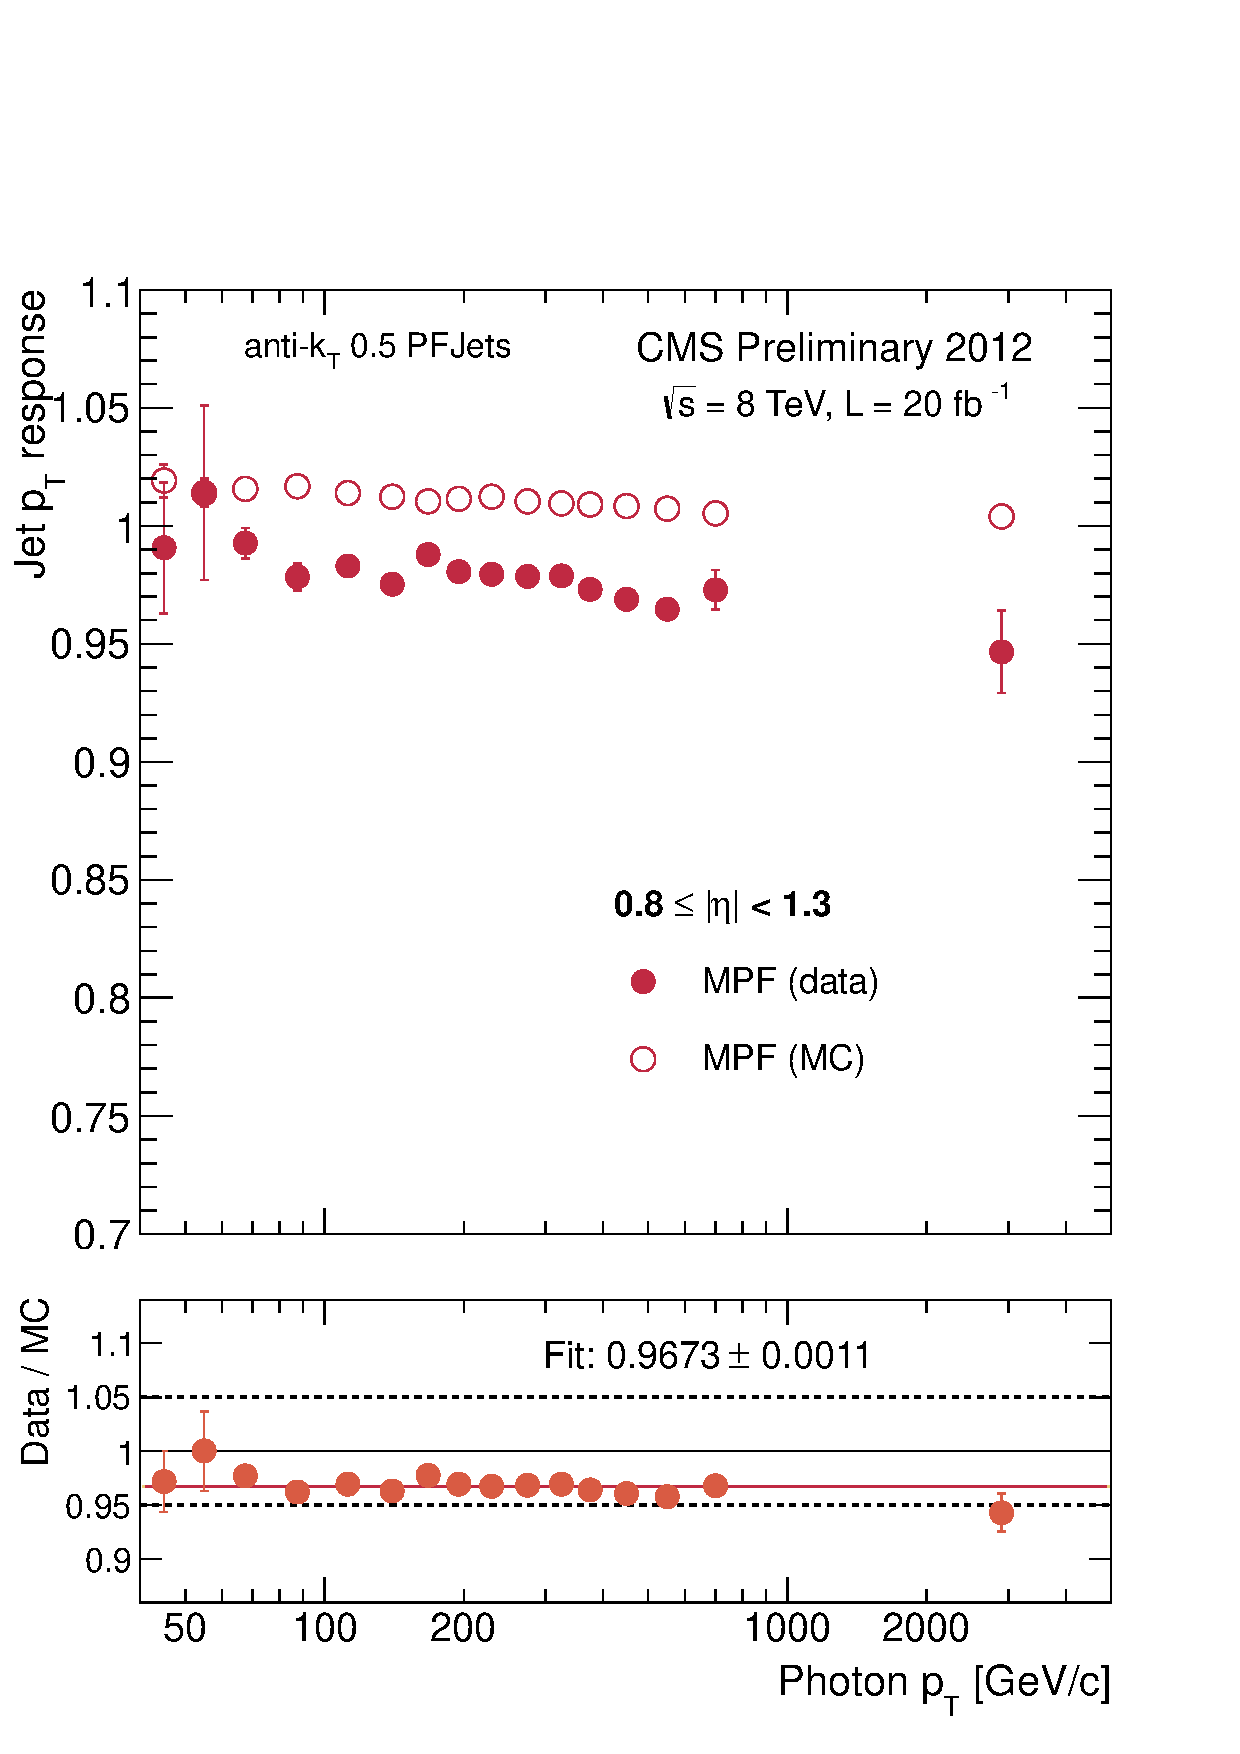
\includegraphics[width=0.45\textwidth]{chapitre4/figs/resp_mpf/response_eta0813_mpf.pdf}}
    \subcaptionbox{\label{fig:mpf_eta1319}}[0.45\textwidth]{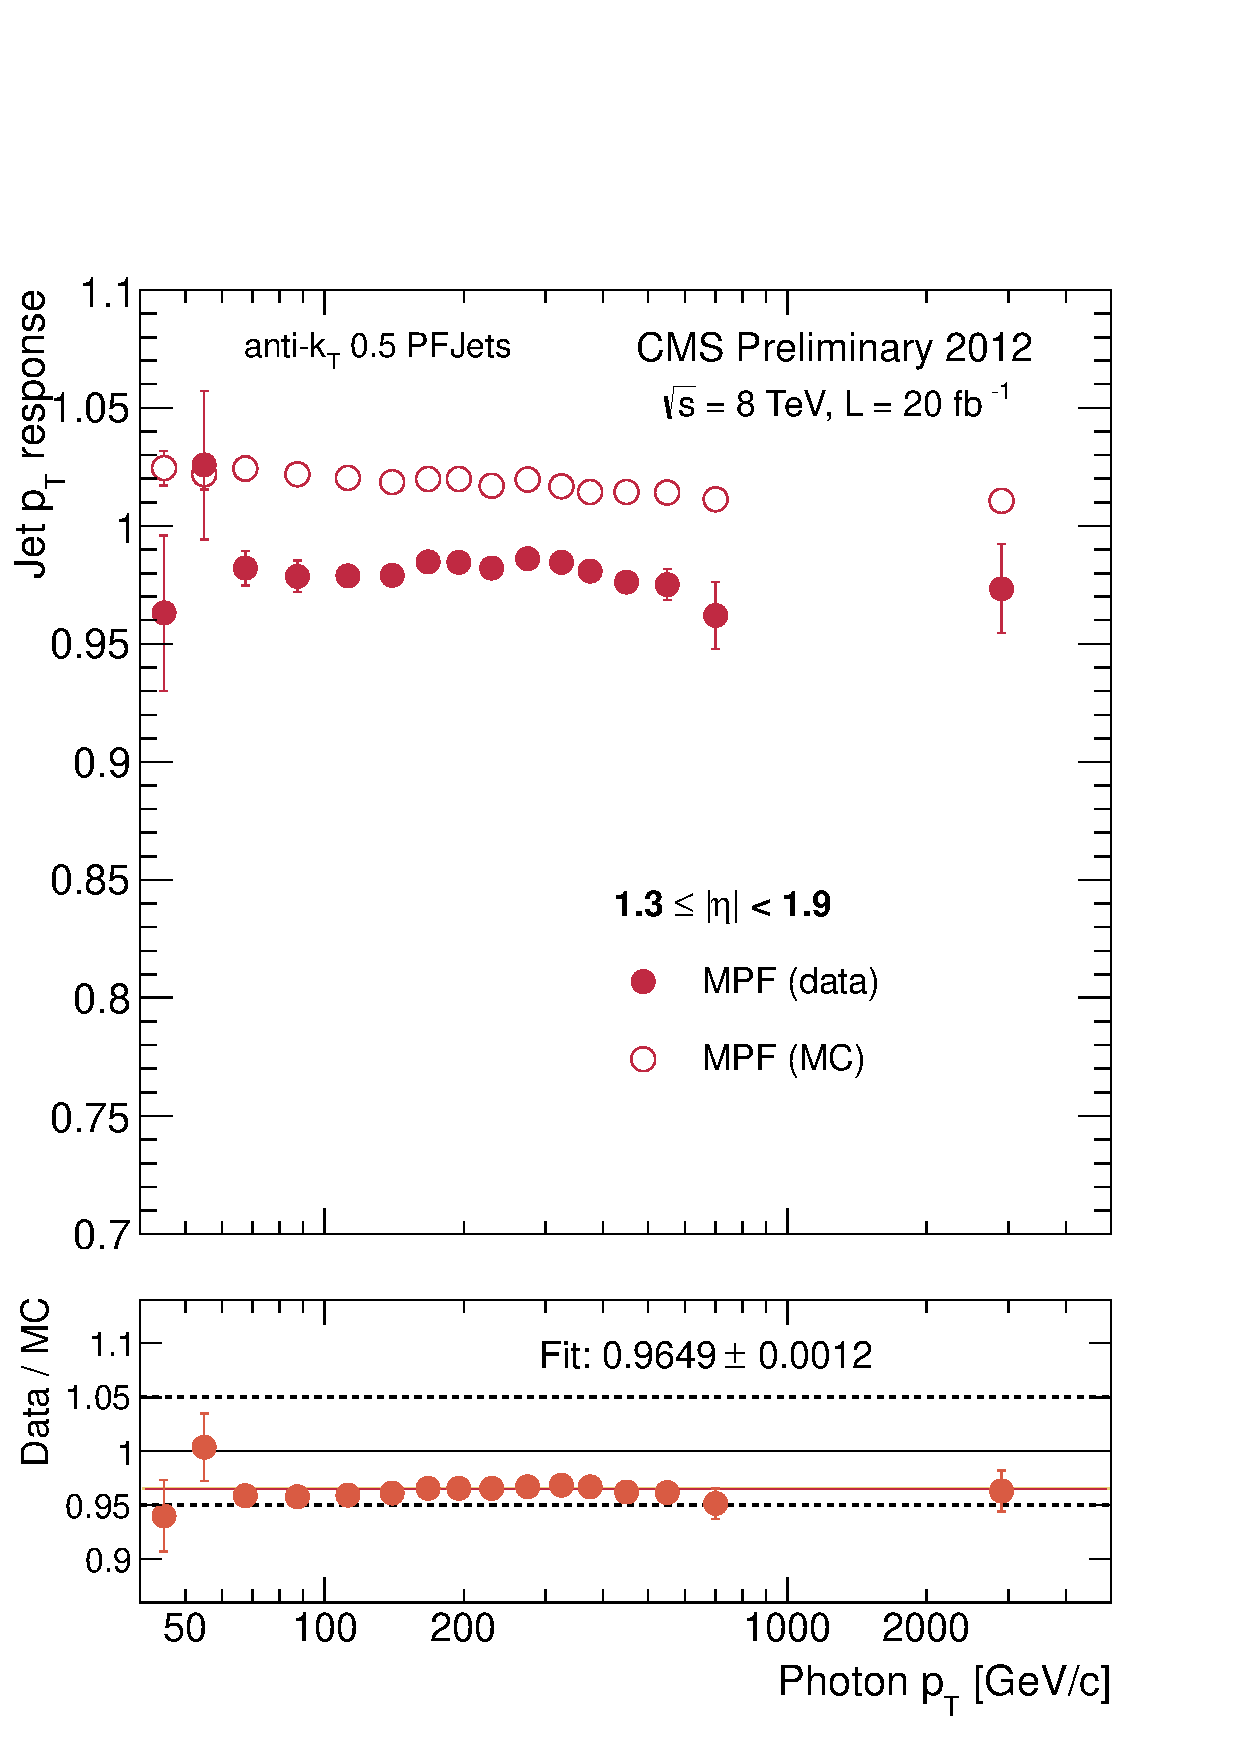
\includegraphics[width=0.45\textwidth]{chapitre4/figs/resp_mpf/response_eta1319_mpf.pdf}}\hfill
    \subcaptionbox{\label{fig:mpf_eta1925}}[0.45\textwidth]{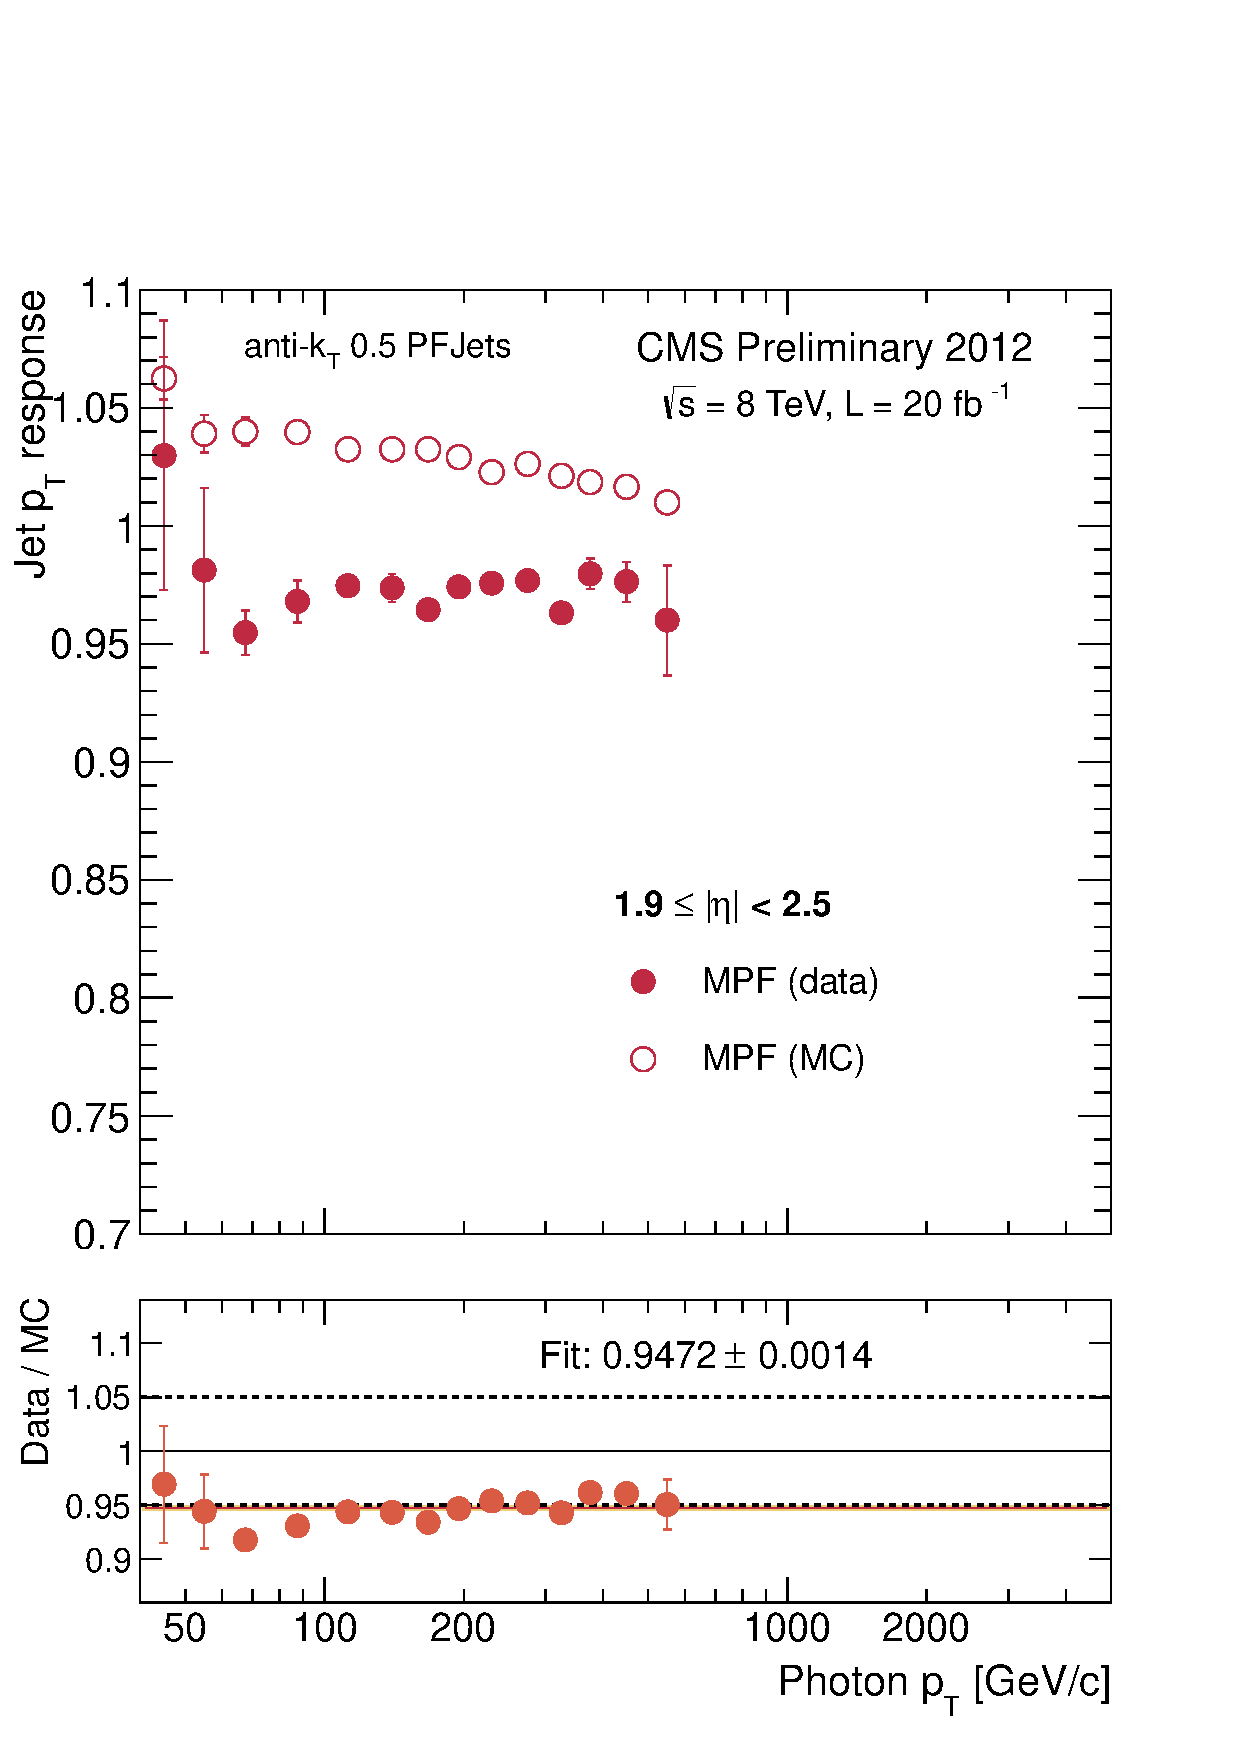
\includegraphics[width=0.45\textwidth]{chapitre4/figs/resp_mpf/response_eta1925_mpf.pdf}}
    \caption{Réponses moyennes pour la méthode MPF, sans extrapolation, pour $\aeta < \num{0.8}$ (\subref{fig:mpf_eta008}), $\num{0.8} \leq \aeta < \num{1.3}$ (\subref{fig:mpf_eta0813}), $\num{1.3} \leq \aeta < \num{1.9}$ (\subref{fig:mpf_eta1319}), et $\num{1.9} \leq \aeta < \num{2.5}$ (\subref{fig:mpf_eta1925}). Le ratio entre les données et la simulation est présenté sous chaque distribution, accompagné d'une interpolation linéaire constante (ligne orange). La bande jaune représente l'erreur sur cette interpolation.}
    \label{fig:mpf_resp}
\end{figure}

% \begin{figure}[p!]
%     \centering
%     \subcaptionbox{\label{fig:reso_mpf_eta008}}[0.45\textwidth]{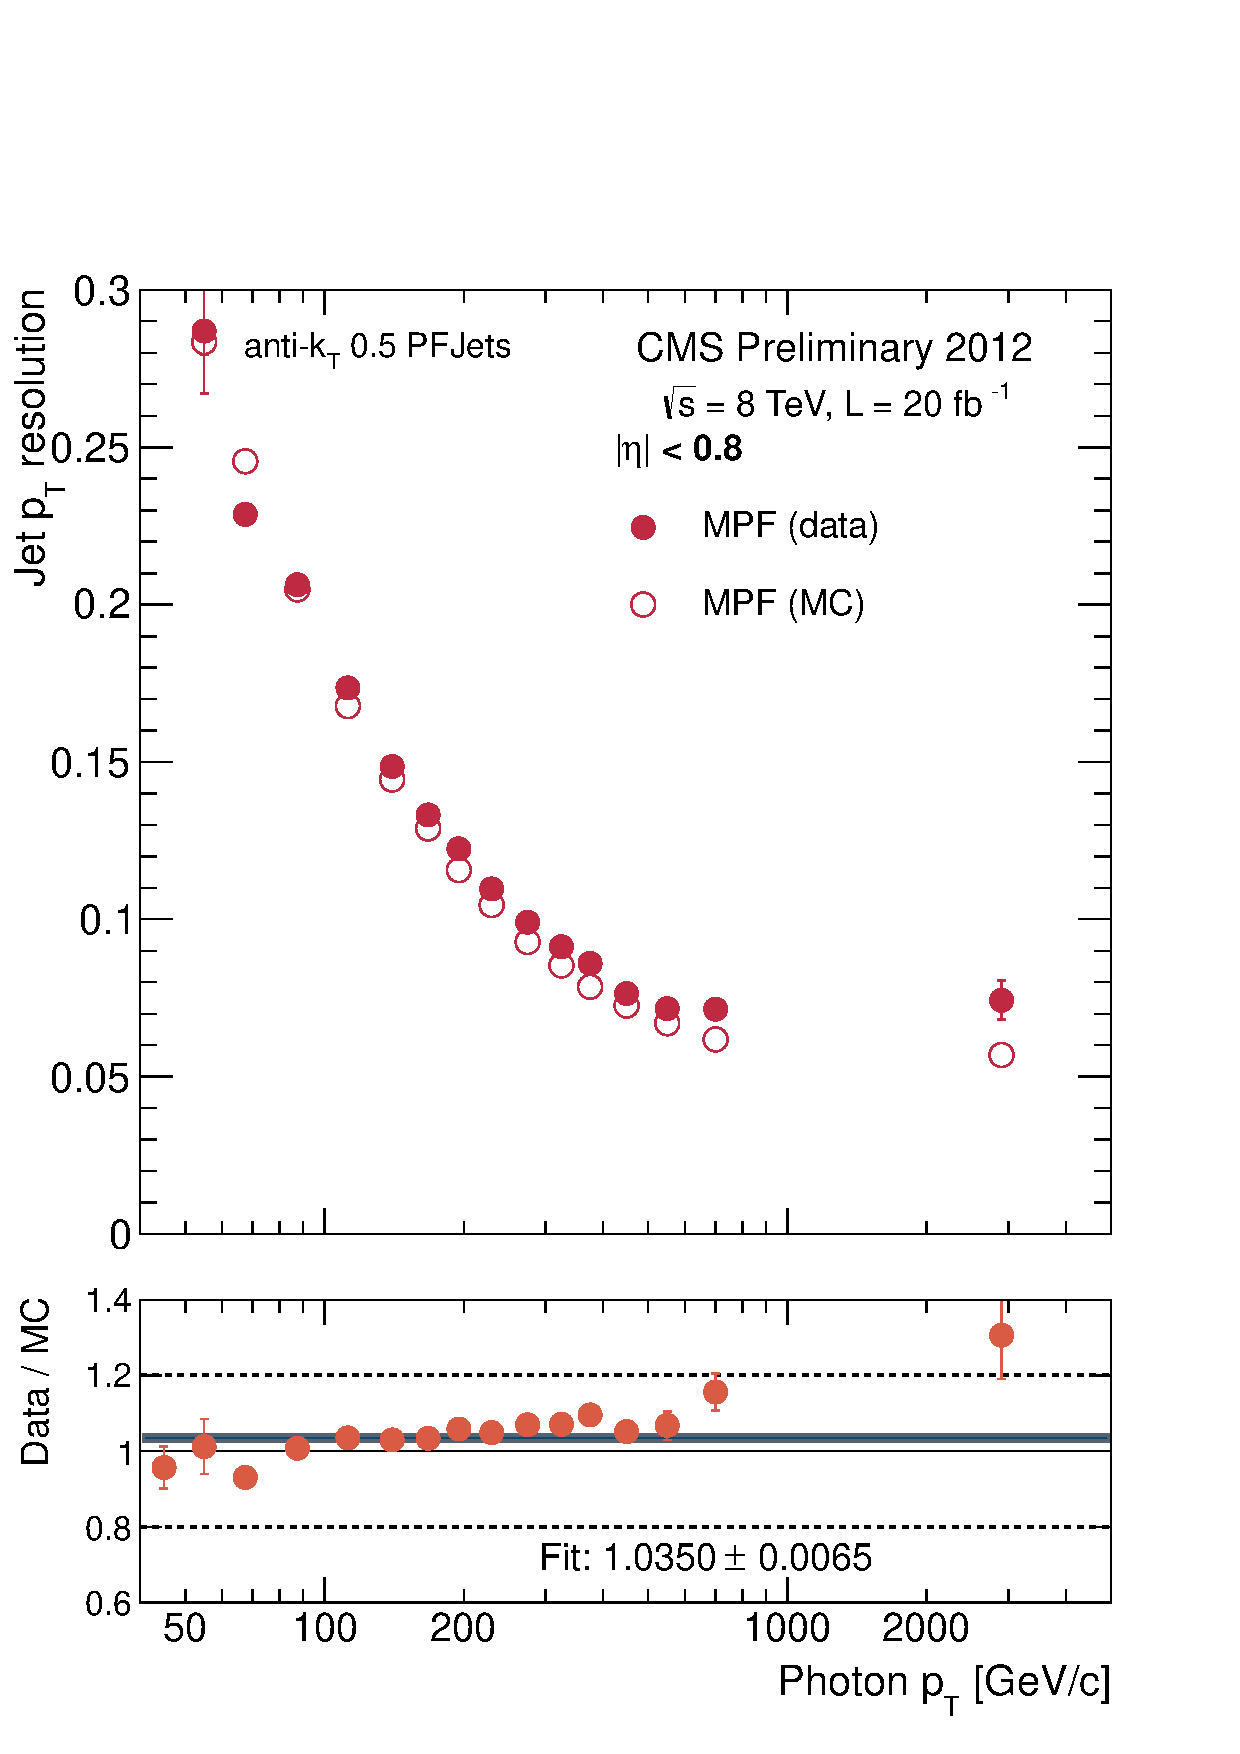
\includegraphics[width=0.45\textwidth]{chapitre4/figs/reso_mpf/resolution_eta008_mpf.pdf}}\hfill
%     \subcaptionbox{\label{fig:reso_mpf_eta0813}}[0.45\textwidth]{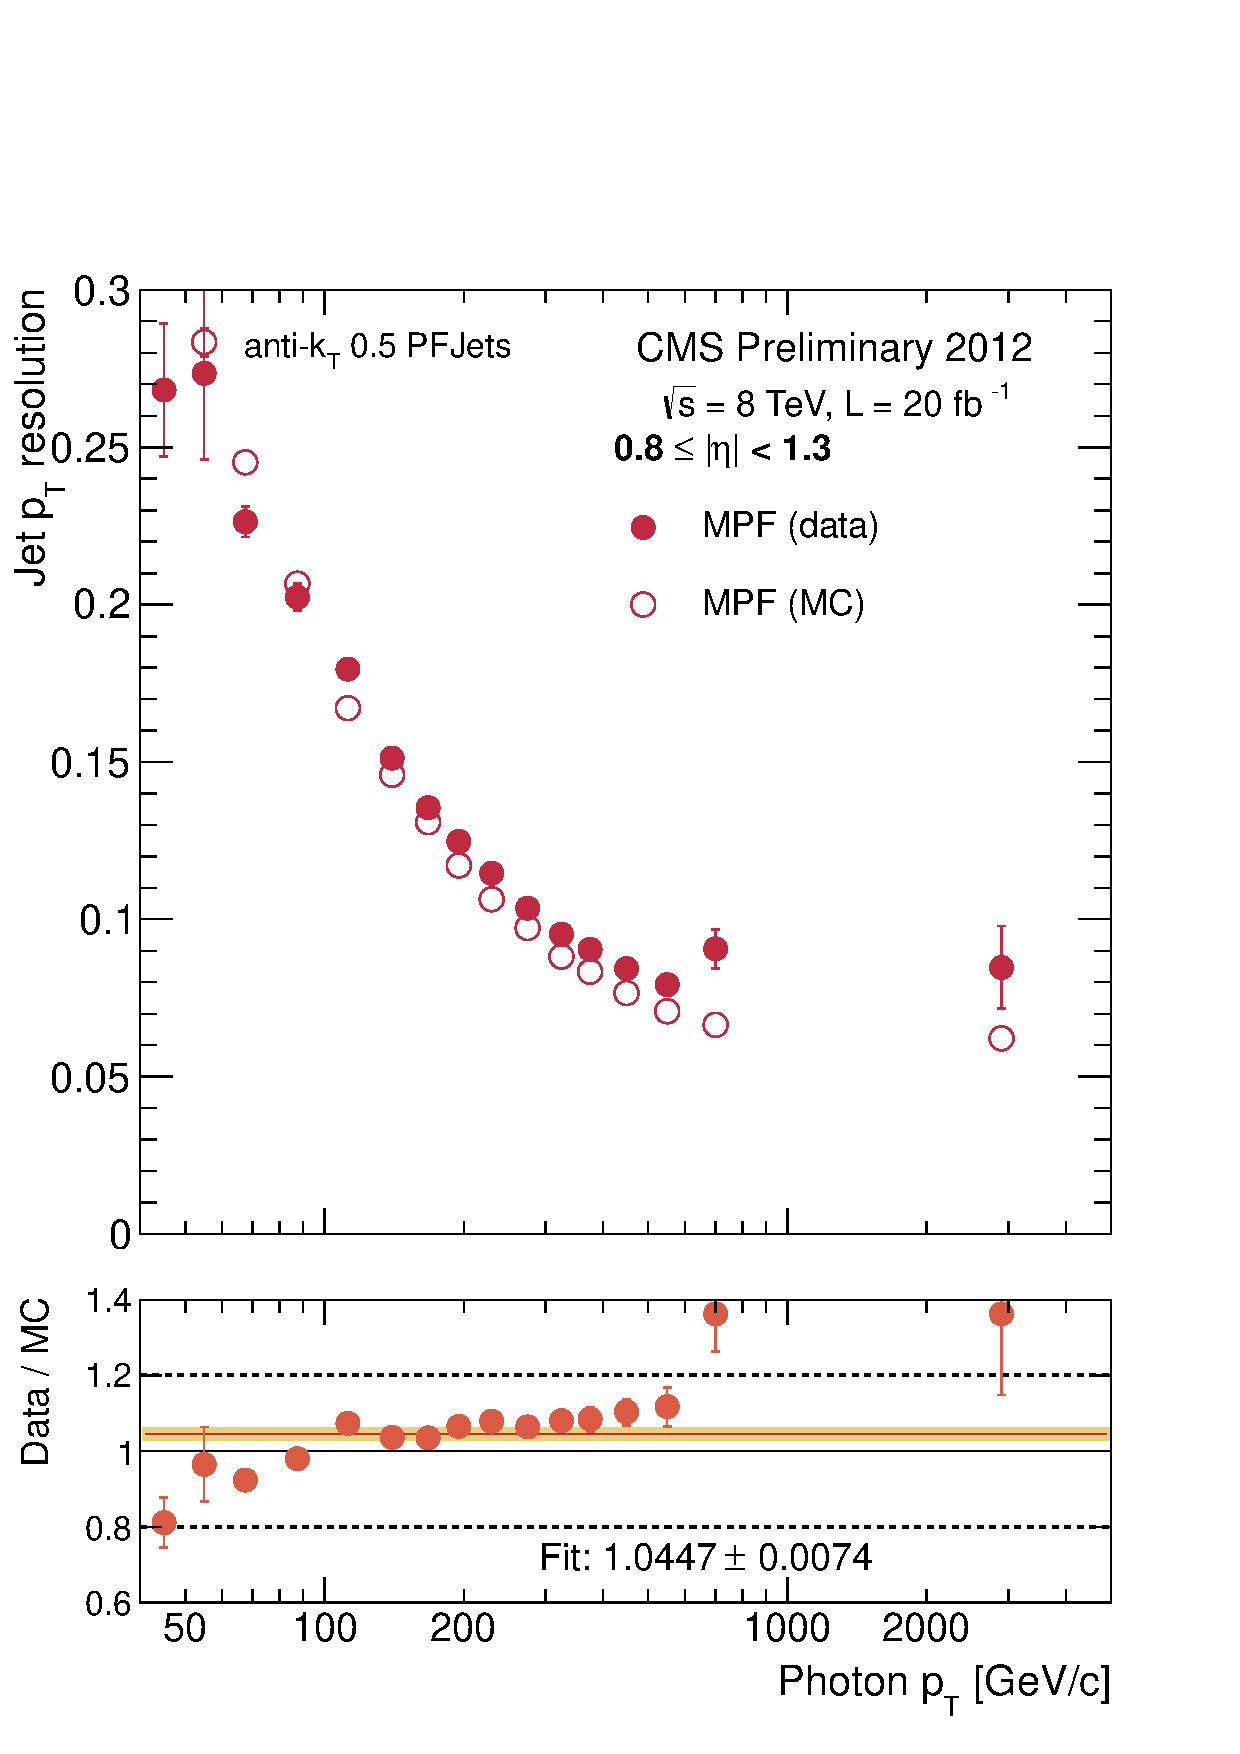
\includegraphics[width=0.45\textwidth]{chapitre4/figs/reso_mpf/resolution_eta0813_mpf.pdf}}
%     \subcaptionbox{\label{fig:reso_mpf_eta1319}}[0.45\textwidth]{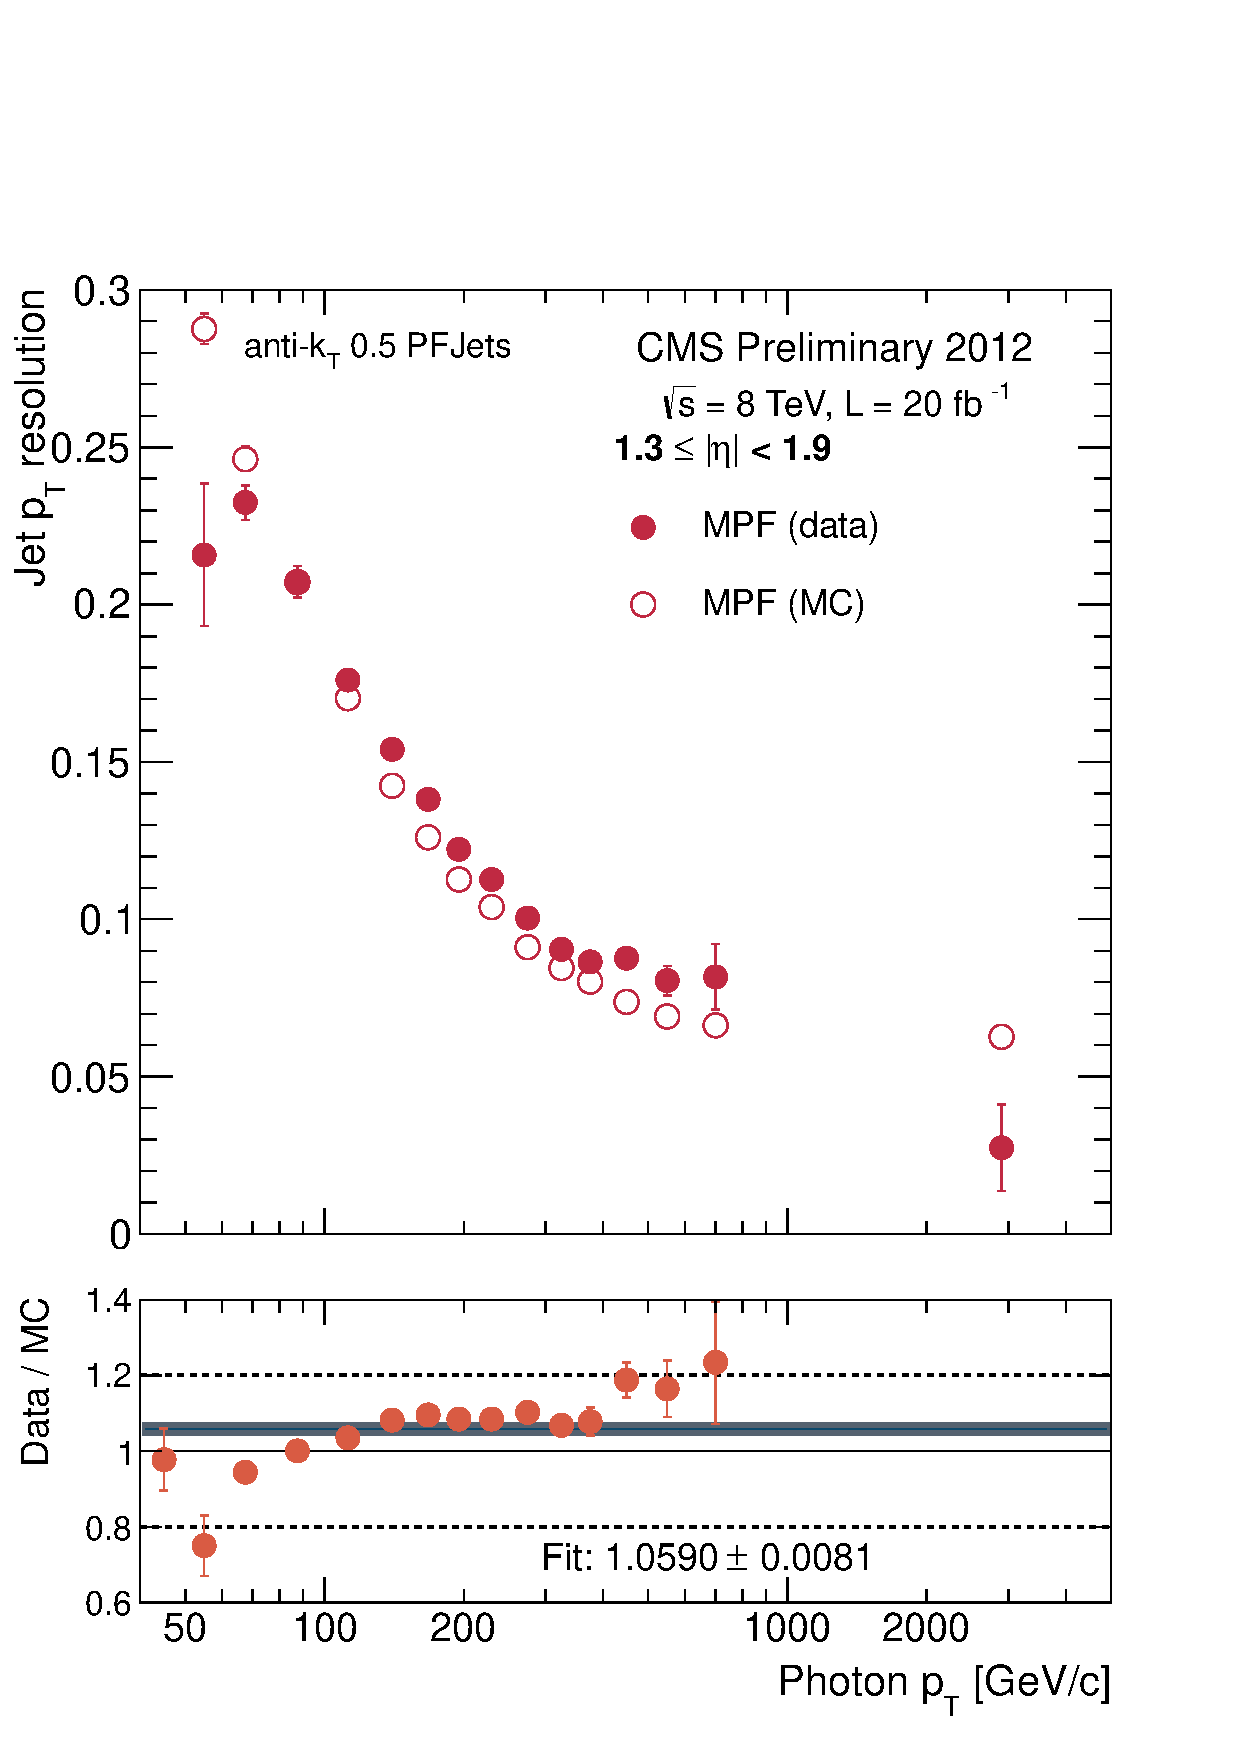
\includegraphics[width=0.45\textwidth]{chapitre4/figs/reso_mpf/resolution_eta1319_mpf.pdf}}\hfill
%     \subcaptionbox{\label{fig:reso_mpf_eta1925}}[0.45\textwidth]{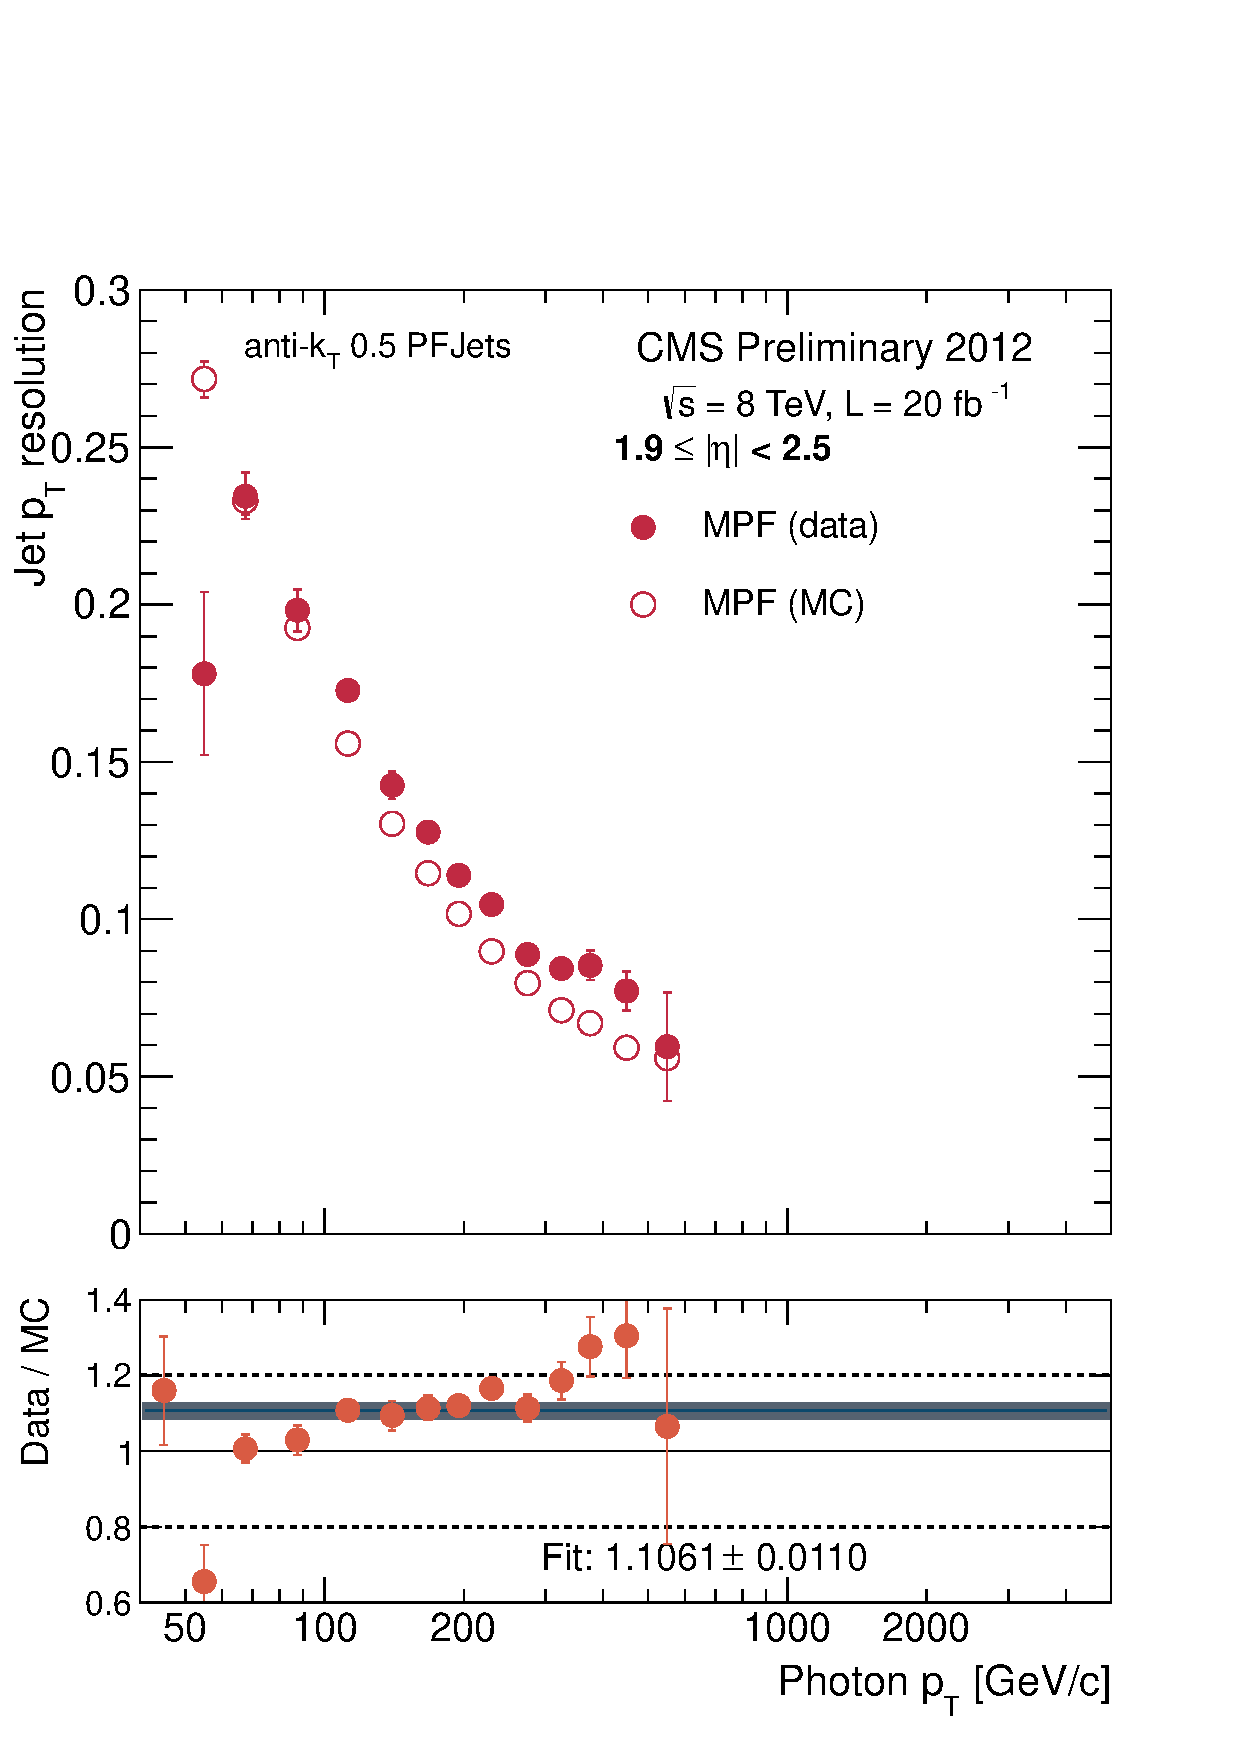
\includegraphics[width=0.45\textwidth]{chapitre4/figs/reso_mpf/resolution_eta1925_mpf.pdf}}
%     \caption{Résolutions pour la méthode MPF, sans extrapolation, pour $\aeta < \num{0.8}$ (\subref{fig:reso_mpf_eta008}), $\num{0.8} \leq \aeta < \num{1.3}$ (\subref{fig:reso_mpf_eta0813}), $\num{1.3} \leq \aeta < \num{1.9}$ (\subref{fig:reso_mpf_eta1319}), et $\num{1.9} \leq \aeta < \num{2.5}$ (\subref{fig:reso_mpf_eta1925}). Le ratio entre les données et la simulation est présenté sous chaque distribution, accompagné d'une interpolation linéaire constante (ligne orange). La bande jaune représente l'erreur sur cette interpolation.}
%     \label{fig:mpf_reso}
% \end{figure}

Par rapport à la méthode de la balance, on constate deux améliorations. Premièrement, les ratios sont plus proches de l'unité, avec des incertitudes comparables. Deuxièmement, ces ratios sont plus stables en fonction de \aeta, particulièrement à haut \aeta, là où le nombre d'événements est réduit.

\begin{figure}[p!]
    \centering
    \subcaptionbox{\label{fig:npv_bal_eta013}}[0.4\textwidth]{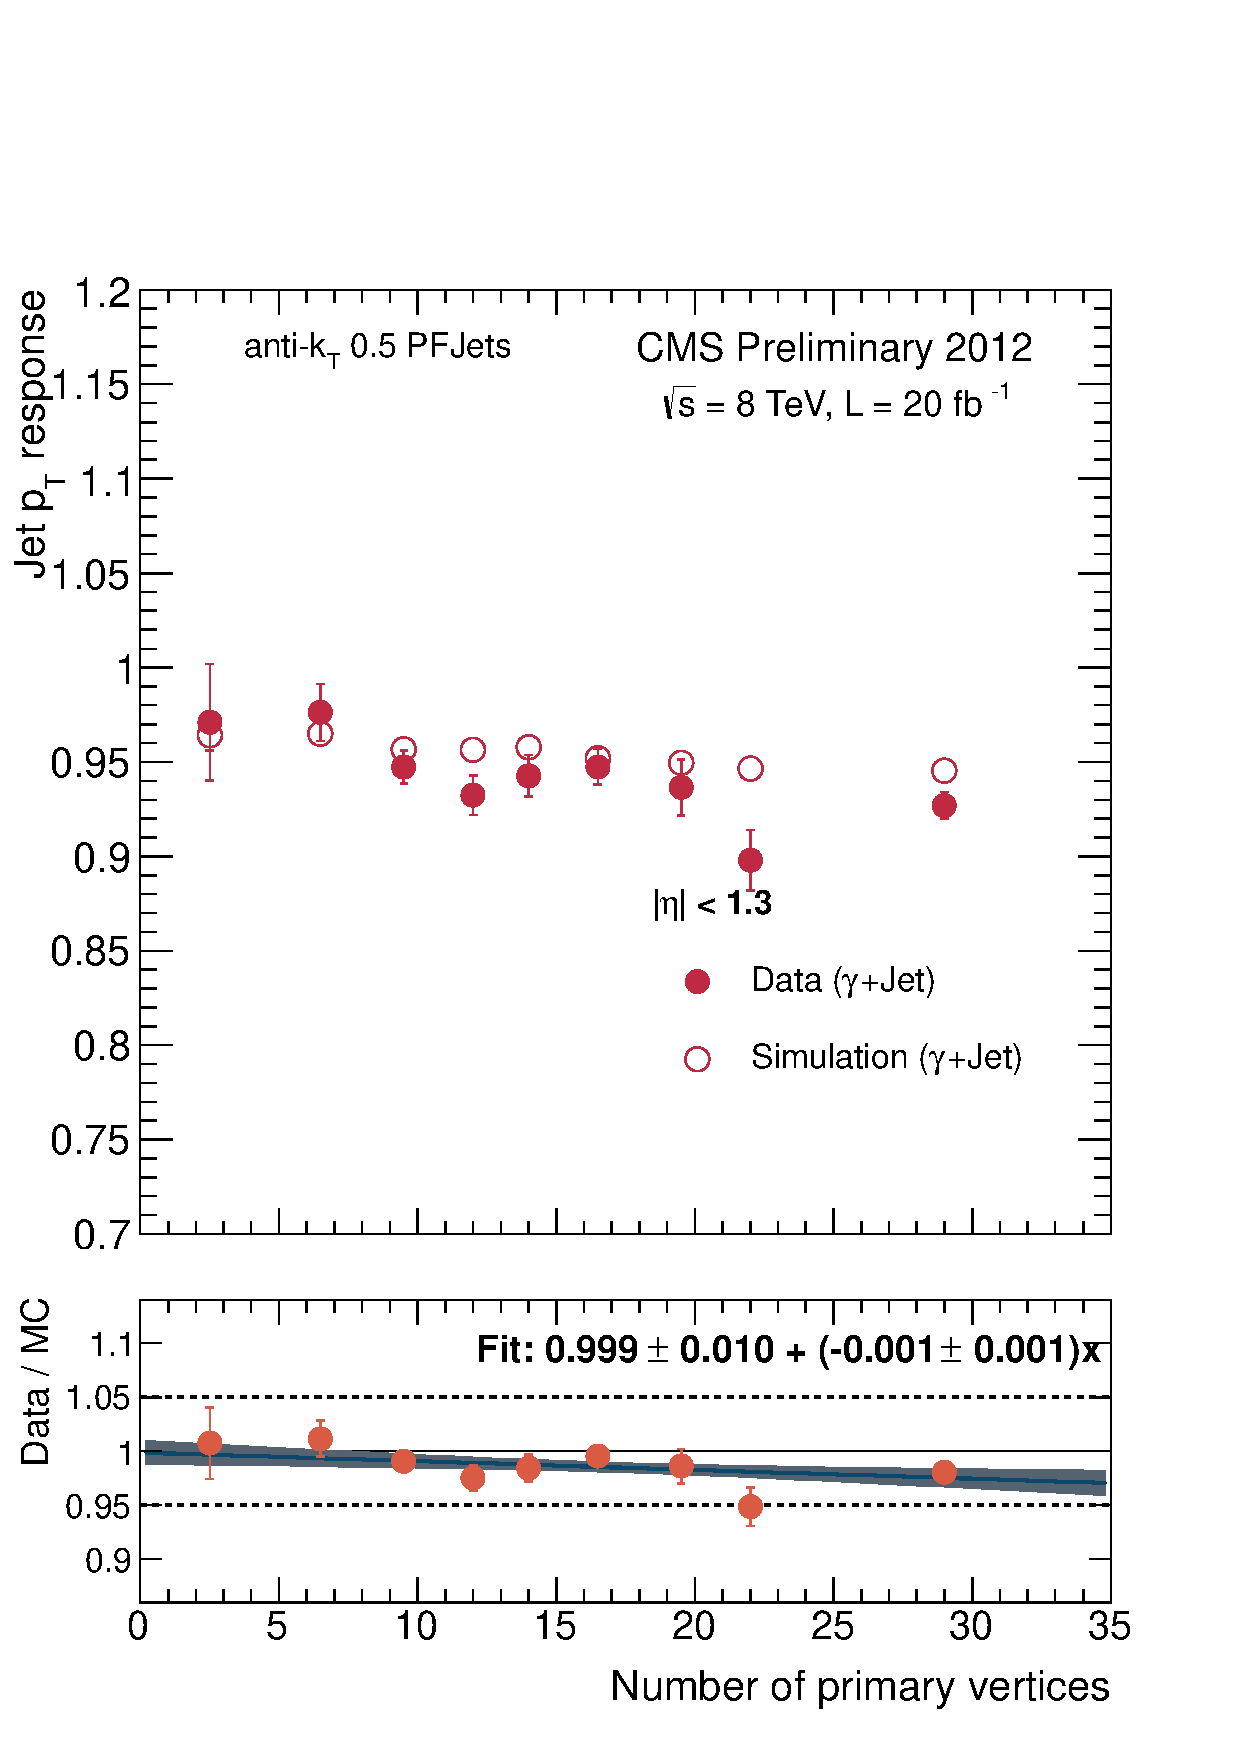
\includegraphics[width=0.4\textwidth]{chapitre4/figs/resp_vs_npv/resp_balancing_eta013_vs_npv_FITLINE.pdf}}\qquad
    \subcaptionbox{\label{fig:npv_mpf_eta013}}[0.4\textwidth]{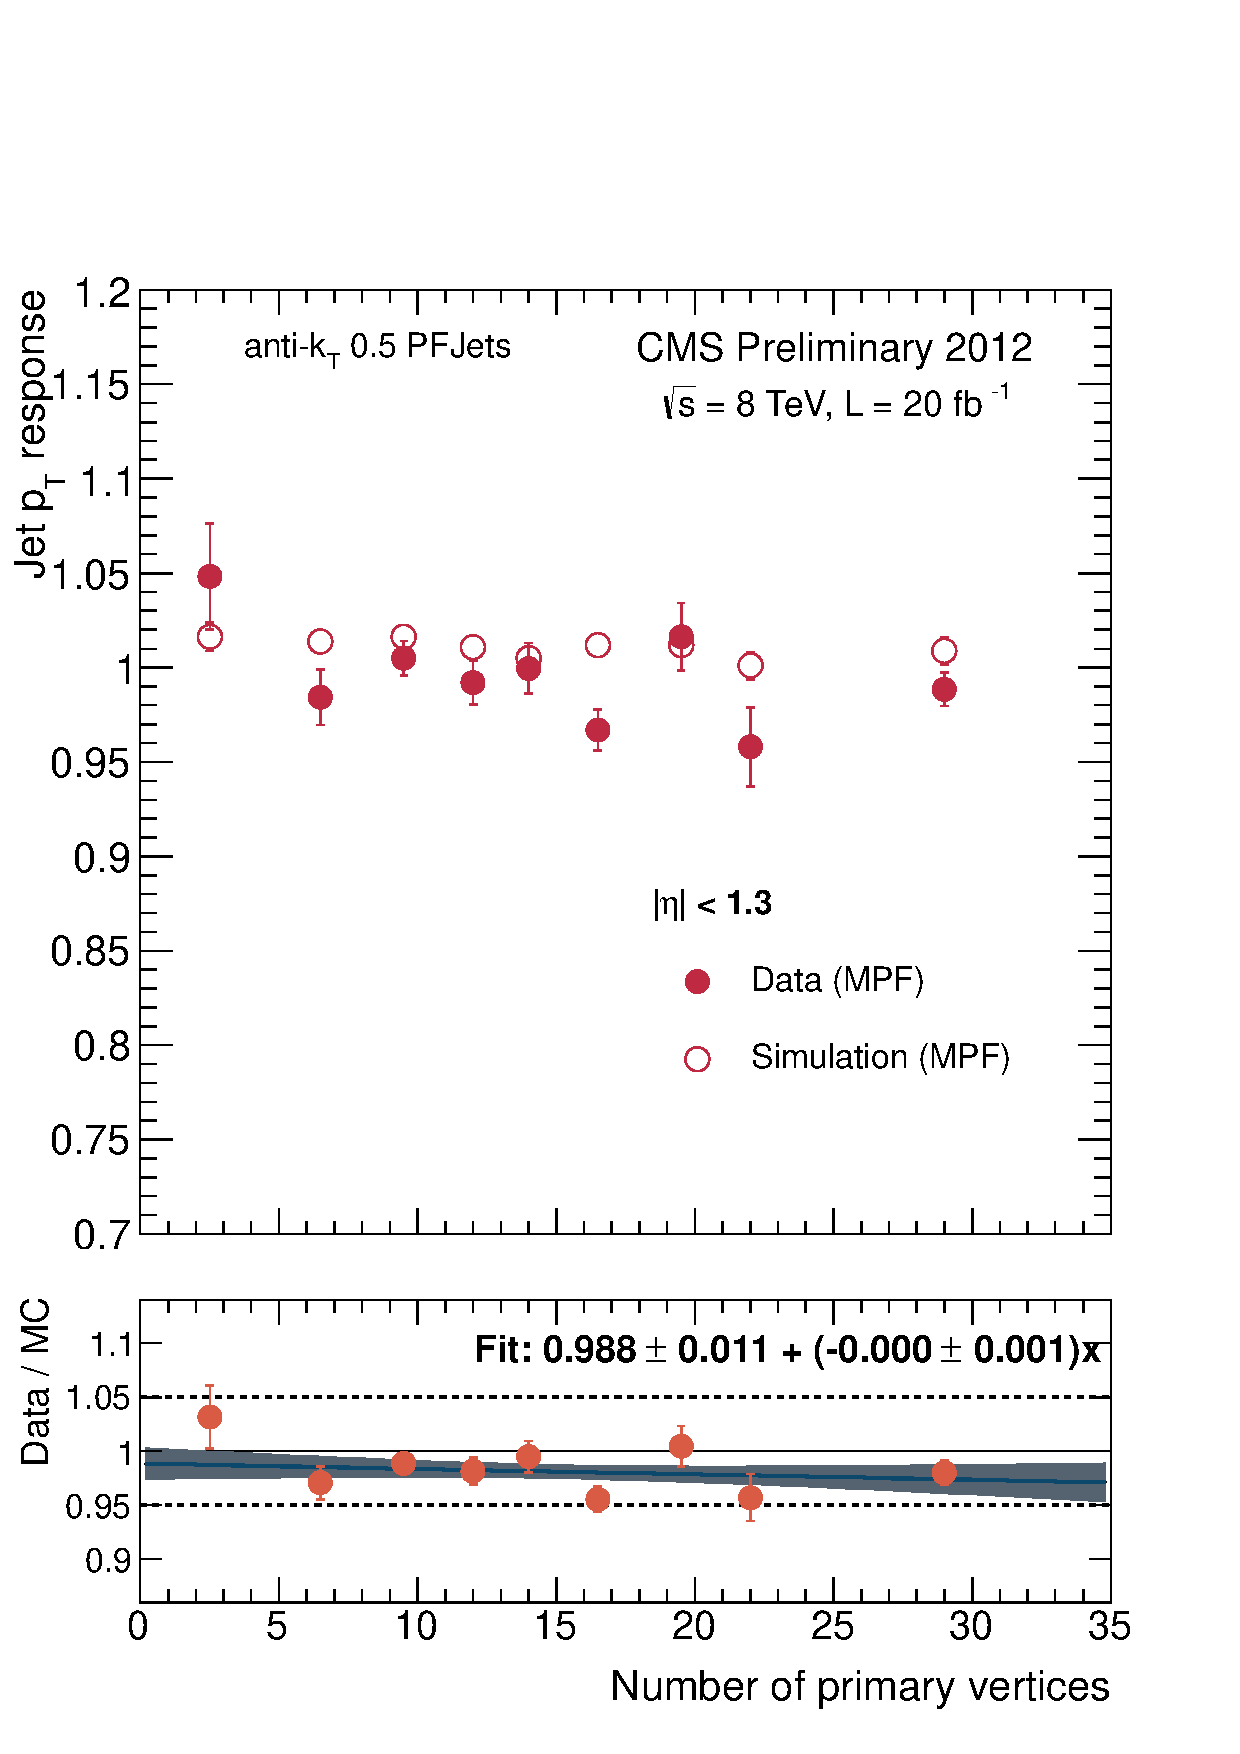
\includegraphics[width=0.4\textwidth]{chapitre4/figs/resp_vs_npv/resp_mpf_eta013_vs_npv_FITLINE.pdf}}
    \caption{Évolution des réponses pour les méthodes de la balance (\subref{fig:npv_bal_eta013}) et MPF (\subref{fig:npv_mpf_eta013}) en fonction du nombre de vertex primaires.}
    \label{fig:resp_vs_npv}
\end{figure}

Ces résultats étaient prévisibles : on a vu précédemment que la méthode était beaucoup moins sensible à l'activité secondaire dans le détecteur, puisqu'elle utilise dès sa définition la totalité de l'impulsion transverse des particules. La présence du \pu n'affecte ainsi pas les performances de la méthode MPF. On peut voir \cref{fig:resp_vs_npv} l'évolution du ratio données sur simulation pour la méthode de la balance et la méthode MPF en fonction du nombre de vertex primaires. On constate que la réponse de la méthode MPF est plus proche de l'unité, et ce même à haut nombre d'interactions. De plus, elle reste stable en fonction du nombre de vertex, contrairement à la méthode de la balance, où on constate une faible évolution.

\subsubsection{Résolution}

Comme évoqué précédemment, on extrait en plus des réponses la résolution sur la réponse des jets. Ces résolutions ne sont pas utilisées dans l'analyse, mais il est néanmoins intéressant de voir les performances de chaque méthode d'extraction de la réponse. La \cref{fig:resolutions} présente les résolutions sur les réponses pour les méthodes de la balance et MPF, pour la classe $\aeta < \num{1.3}$. On constate que la différence de résolution entre les données et la simulation est d'environ \SI{20}{\percent} pour la méthode de la balance, et de seulement \tilde\SI{5}{\percent} pour la méthode MPF.

\begin{figure}[tbp] \centering
    \subcaptionbox{Méthode de la balance}[0.4\textwidth]{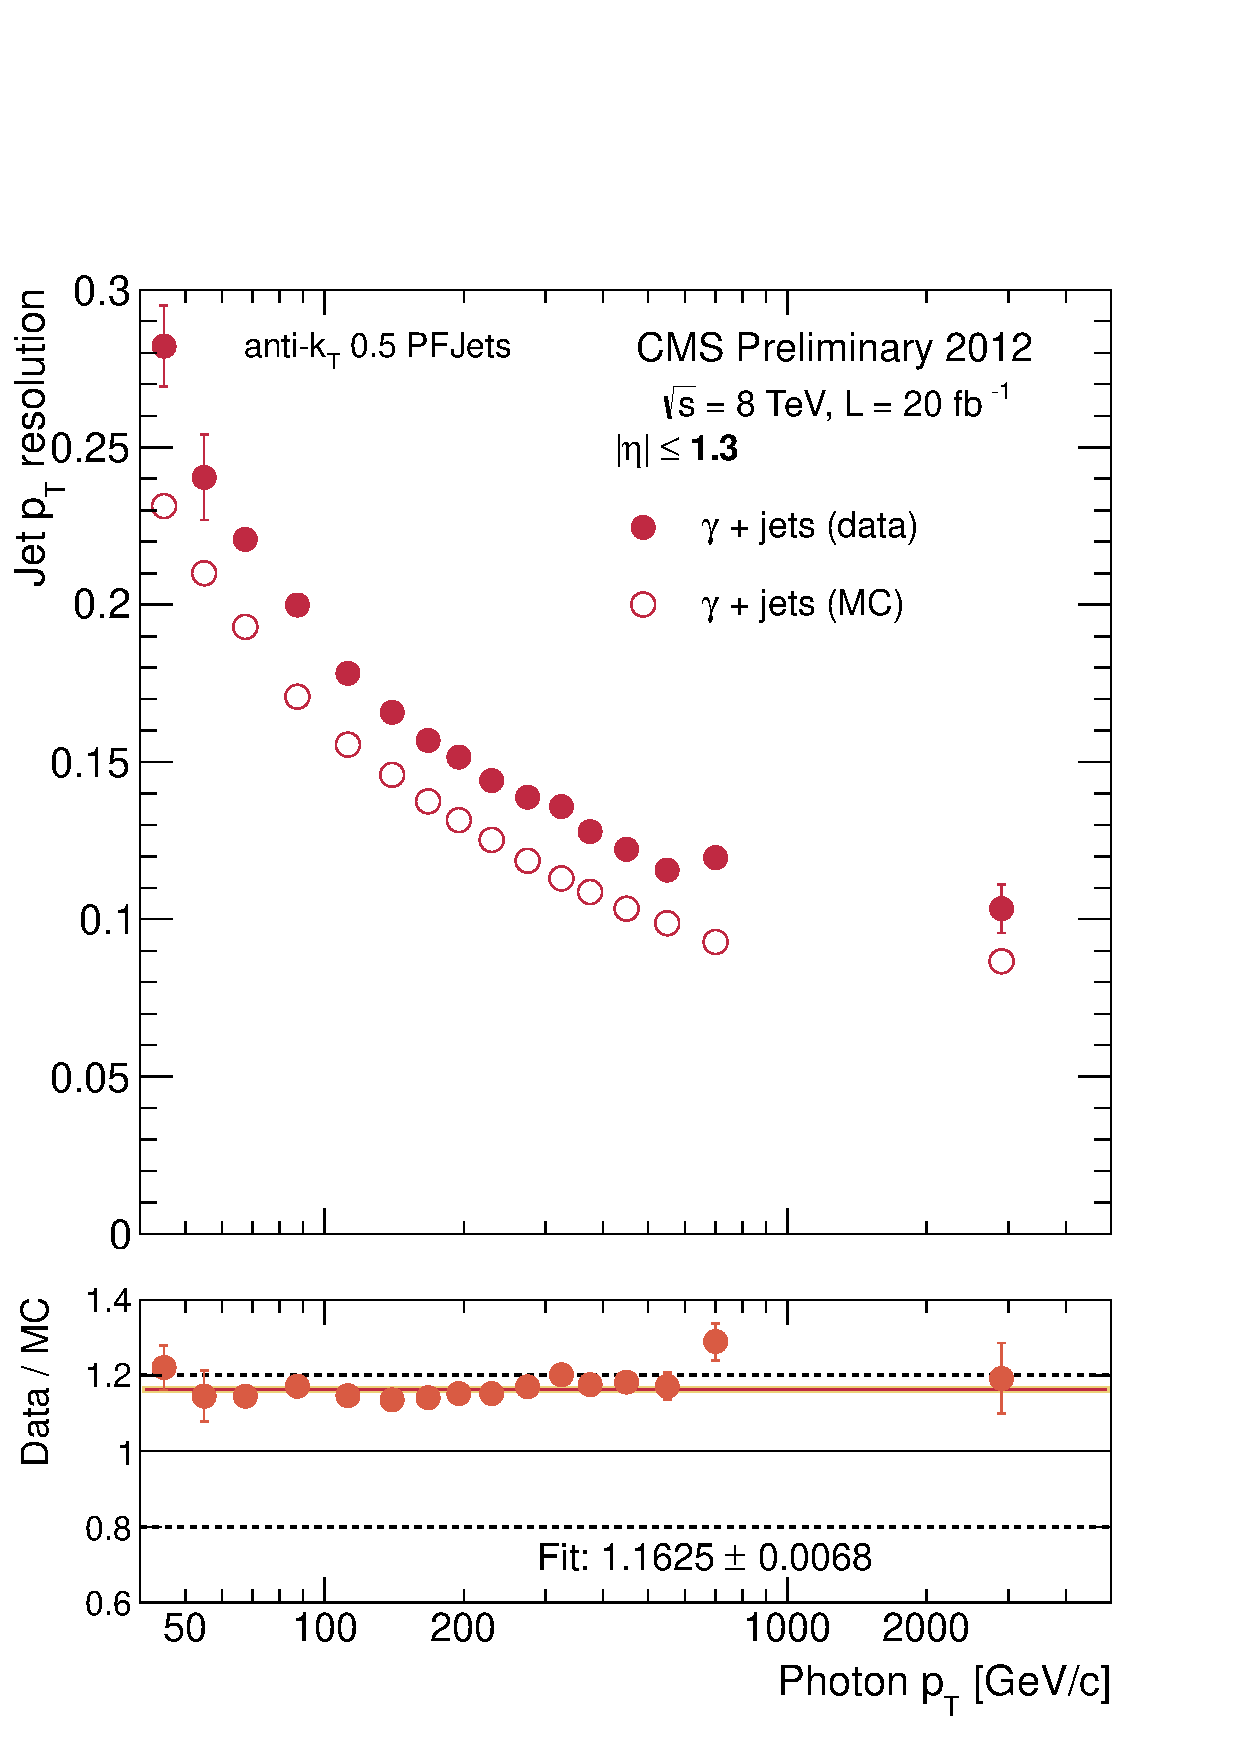
\includegraphics[width=0.4\textwidth]{chapitre4/figs/reso_balancing/resolution_eta013_balancing.pdf}} \qquad
    \subcaptionbox{Méthode MPF}[0.4\textwidth]{\includegraphics[width=0.4\textwidth]{chapitre4/figs/reso_mpf/resolution_eta013_mpf.pdf}}
    \caption{Résolutions sur la réponse des jets pour les méthodes de la balance et MPF, pour $\aeta < \num{1.3}$.}
    \label{fig:resolutions}
\end{figure}

\subsection{Extraction des corrections résiduelles}

\begin{figure}[tbp]
  \centering
  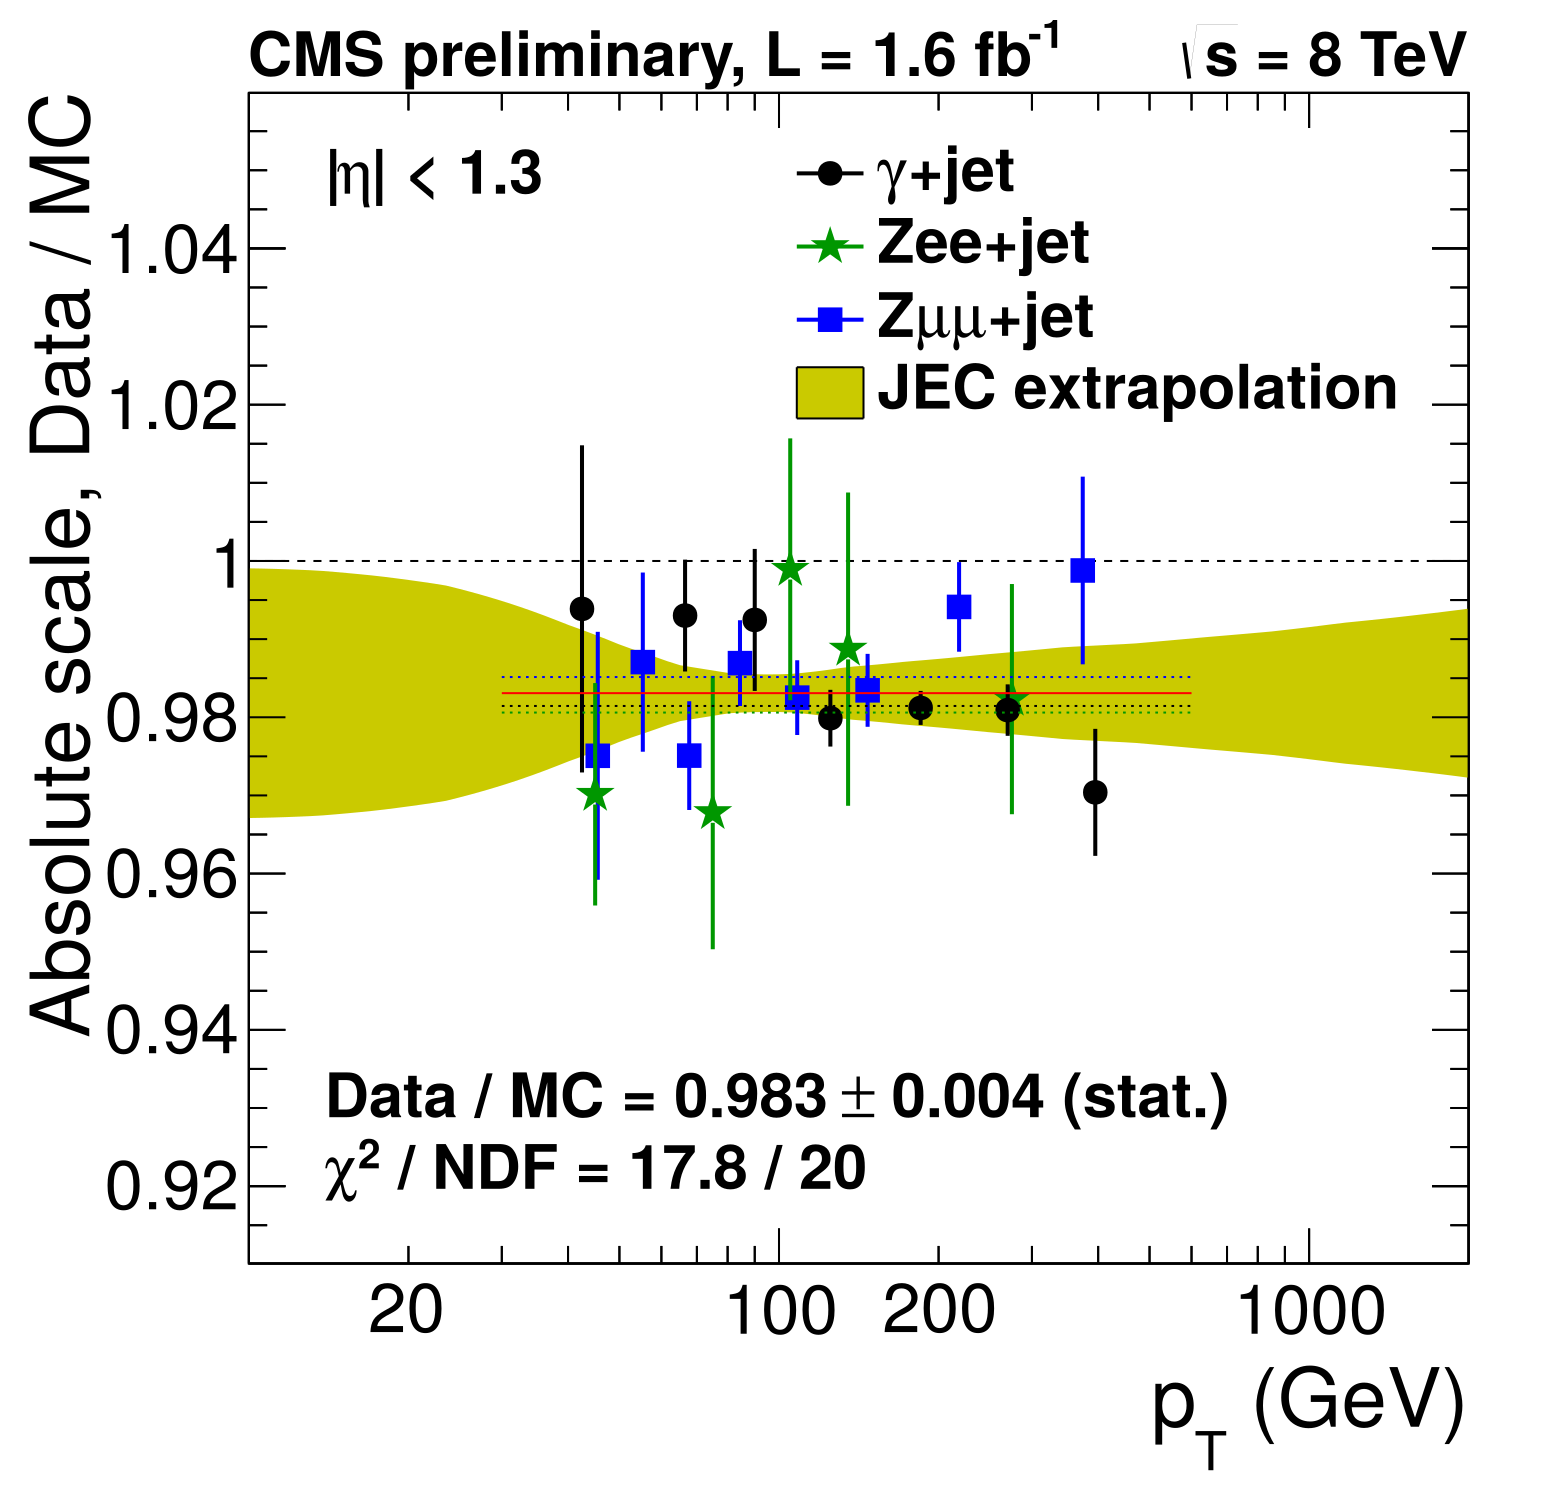
\includegraphics[width=0.65\textwidth]{chapitre4/figs/jec_residuals_combined.pdf}
  \caption{Extraction des facteurs de corrections résiduels grâce à une combinaison entre les analyses $\PZ \rightarrow \Pmuon \APmuon$ + jets, \PZ $\rightarrow$ \Pelectron \APelectron + jets et \Pphoton + jets.}
  \label{fig:jec_residuals_combined}
\end{figure}


Afin d'obtenir les corrections résiduelles finales, on combine les résultats de l'analyse \Pphoton + jets avec les analyses $\PZ \rightarrow \Pmuon \APmuon$ + jets et \PZ $\rightarrow$ \Pelectron \APelectron + jets. La \cref{fig:jec_residuals_combined} présente la combinaison entre ces trois analyses. Une interpolation globale entre les trois résultats permet d'obtenir les facteurs de corrections résiduelles officiels. Cette interpolation est étendue aux zones à bas et haut $p_T$, non couvertes par les analyses : les incertitudes liées à cette extrapolation sont utilisées comme source d'erreurs systématiques, comme présenté \cref{sec:jec_uncertainties}.

\bigskip

On constate que les résultats des trois analyses sont compatibles entre eux. On extrait ainsi un ratio données sur simulation de \SI{0.983 \pm 0.004}{}. La même procédure est reproduite pour chaque classe en \aeta. Les corrections résiduelles ainsi dérivées sont utilisées par toute la collaboration.

\subsection{Test d'intégrité}


\begin{figure}[tbp]
    \centering
    \subcaptionbox{Sans corrections résiduelles\label{fig:mpf_no_residuals_eta013_pt_210_250}}[0.45\textwidth]{\includegraphics[width=0.45\textwidth]{chapitre4/figs/resp_mpf_eta013_ptPhot_210_250.pdf}} \qquad
    \subcaptionbox{Avec corrections résiduelles\label{fig:mpf_residuals_eta013_pt_210_250}}[0.45\textwidth]{\includegraphics[width=0.45\textwidth]{chapitre4/figs/resp_mpf_eta013_ptPhot_210_250_residuals.pdf}}
    \caption{Réponses pour la méthode MPF pour une en \ptg entre 210 - \SI{250}{\GeV}, pour $\aeta < \num{1.3}$, avec et sans corrections résiduelles.}
    \label{fig:comp_mpf_residuals}
\end{figure}

Les corrections résiduelles déterminées, on peut maintenant vérifier l'effet produit. Pour cela, on recommence l'analyse en corrigeant les jets avec tous les niveaux de corrections disponibles, et on extrait les nouveaux ratios des réponses. Si tout est parfait, on s'attend à obtenir des ratios proche de 1.

La \cref{fig:comp_mpf_residuals} présente la distribution des réponses pour une classe en \ptg entre 210 - \SI{250}{\GeV} pour la méthode MPF, sans corrections résiduelles (\subref{fig:mpf_no_residuals_eta013_pt_210_250}) et avec (\subref{fig:mpf_residuals_eta013_pt_210_250}). On constate bien une amélioration de la réponse moyenne sur les données grâce à l'ajour des corrections résiduelles : le décalage observé précédemment entre les distributions des réponses données et simulation a disparu. Afin de confirmer cette observation, on peut voir \cref{fig:comp_mpf_residuals_2} les distributions des réponses moyennes après application des corrections résiduelles. Comme prévu, le ratio est amélioré par rapport au \cref{tab:res_mpf}, ce qui permet de valider nos corrections. Le ratio n'est cependant pas égal à 1, mais cet écart est néanmoins couvert par les erreurs systématiques détaillées \cref{sec:jec_uncertainties}.

\begin{figure}[tbp]
    \centering
    \subcaptionbox{\label{fig:resp_mpf_residuals_eta008}}[0.45\textwidth]{\includegraphics[width=0.45\textwidth]{chapitre4/figs/resp_mpf_residuals/response_eta008_mpf.pdf}} \qquad
    \subcaptionbox{\label{fig:resp_mpf_residuals_eta0813}}[0.45\textwidth]{\includegraphics[width=0.45\textwidth]{chapitre4/figs/resp_mpf_residuals/response_eta0813_mpf.pdf}}
    \caption{Réponses moyennes pour la méthode MPF, après corrections résiduelles, pour deux classes \aeta : $\num{< 0.8}$ et \num{0.8} - \num{1.3}.}
    \label{fig:comp_mpf_residuals_2}
\end{figure}

\section{Corrections résiduelles dépendantes de la saveur des jets}

Tout au long de ce chapitre, les corrections en énergie des jets ont été dérivées sans tenir compte de la saveur du jet. Il est cependant tout à fait raisonnable d'imaginer que la réponse d'un jet puisse dépendre de sa saveur. Cette hypothèse est en effet confirmée, comme on a pu le voir \cref{fig:jet_flavor_resp}. Actuellement, cette différence de réponse est prise en compte dans les incertitudes systématiques, en utilisant comme valeur la différence entre la réponse des jets légers et les jets de gluons, qui encadrent la réponse des jets de \Pcharm et \Pbottom (\tilde\SI{2}{\percent}, voir \cref{fig:flavor_response}).

Il est donc intéressant de regarder comment varient les différents niveaux de corrections appliqués aux jets en fonction de la saveur de ces jets. Des études sont actuellement en cours dans CMS, et cette section aborde rapidement les premières études préliminaires réalisées pour les corrections résiduelles.

\subsection{Détermination de la saveur d'un jet}

\begin{figure}[tbp] \centering
    \subcaptionbox{\label{fig:flavor_response}}[0.49\textwidth]{\includegraphics[width=0.49\textwidth]{chapitre4/figs/flavor_response.pdf}}
    \subcaptionbox{\label{fig:qgd}}[0.48\textwidth]{\includegraphics[width=0.48\textwidth]{chapitre4/figs/qgd.pdf}}
    \caption{(\subref{fig:flavor_response}) Facteurs de corrections dépendants de la saveur dérivées à l'aide de la vérité Monte-Carlo. (\subref{fig:qgd}) Valeur du discriminant quark\-/gluon pour des événements simulées (histogrammes) et pour les données 2012 (points noirs). Les jets de quarks ont majoritairement une valeur du discriminant proche de 1.}
\end{figure}

Le parton de l'événement dur responsable de la création d'un jet permet de définir sa saveur. On dispose déjà d'un algorithme permettant d'identifier les jets provenant d'un quark \Pbottom, présenté \cref{sec:b_tagging}. Il s'avère que cet algorithme est aussi capable d'identifier les jets provenant d'un quark \Pcharm, ces jets ayant des caractéristiques similaires aux jets de \Pbottom. Il reste donc à différencier les jets provenant d'un gluon de ceux provenant d'un quark léger (\Pup, \Pdown, \Pstrange). On dispose pour cela d'un algorithme spécialisé, le discriminant quark\-/gluon (QGD, \emph{Quark-Gluon discriminant}) \citep{CMS-PAS-JME-13-002}, qui permet de séparer les jets provenant d'un quark de ceux provenant d'un gluon. Cet algorithme exploite plusieurs différences entre ces jets :
\begin{itemize}
  \item Le nombre de particules chargées constituant les jets de gluons est plus important que dans les jets de quarks, puisque les gluons, contrairement aux quarks, portent une "double" charge de couleur \citep{Dremin:2000wt}.
  \item Pour des raisons similaires, l'étalement du jet dans le plan $(\eta, \phi)$ est plus important pour les jets provenant de gluons que pour les jets provenant de quarks.
\end{itemize}

La \cref{fig:qgd} présente les performances de l'algorithme. Un grand pouvoir de séparation entre jets de quarks et jets de gluons est obtenu, les jets de quarks ayant majoritairement une valeur du discriminant proche de 1, alors que les jets de gluons sont plus proches de 0.

\begin{figure}[p!] \centering
    \subcaptionbox{jets légers}[0.48\textwidth]{\includegraphics[width=0.48\textwidth]{chapitre4/figs/flavor/2DTaggingPlan_uds_ptPhot_100_800_stageM2.pdf}}
    \subcaptionbox{jets de \Pcharm}[0.48\textwidth]{\includegraphics[width=0.48\textwidth]{chapitre4/figs/flavor/2DTaggingPlan_c_ptPhot_100_800_stageM2.pdf}} \\
    \subcaptionbox{jets de \Pbottom}[0.48\textwidth]{\includegraphics[width=0.48\textwidth]{chapitre4/figs/flavor/2DTaggingPlan_b_ptPhot_100_800_stageM2.pdf}}
    \subcaptionbox{jets de gluons}[0.48\textwidth]{\includegraphics[width=0.48\textwidth]{chapitre4/figs/flavor/2DTaggingPlan_g_ptPhot_100_800_stageM2.pdf}}
    \caption{Distribution de la fraction des différentes saveurs de jets dans le plan 2D. Une couleur bleue signifie une zone pauvre en jets, et une couleur rouge riche en jets. Les cadres noires représentent les zones sélectionnées enrichies en saveur.}
    \label{fig:2d_zones}
\end{figure}

\begin{table}[p!] \centering
  \begin{tabular}{@{}lcccc@{}} \toprule
     %\multirow{2}{*}{Zone} & \multicolumn{4}{c}{Fraction (\%)} \\ \cmidrule{2-5}
     & \multicolumn{4}{c}{Fraction (\%)} \\ \cmidrule{2-5}
     Zone & \Pup \Pdown \Pstrange & \Pcharm & \Pbottom & gluon \\ \midrule
     enrichie en \Pup \Pdown \Pstrange  & \num{89.3} & \num{7.0} & \num{0.1} & \num{3.6} \\
     enrichie en \Pcharm & \num{22.5} & \num{66.1} & \num{8.5} & \num{2.9} \\
     enrichie en \Pbottom & \num{6.6} & \num{17.1} & \num{66.1} & \num{10.2} \\
     enrichie en gluons & \num{49.8} & \num{9.4} & \num{0.8} & \num{40.0} \\ \bottomrule
  \end{tabular}
  \caption{Fractions des différentes saveurs de jets pour chacune des zones enrichies.}
  \label{tab:2d_zones}
\end{table}

\bigskip

On combine l'algorithme d'étiquetage des jets de \Pbottom avec le discriminant quark\-/gluon afin d'extraire la saveur d'un jet. On créé pour cela un plan 2D avec un abscisse la valeur de sortie de l'algorithme d'étiquetage des jets de \Pbottom (CSV), et en ordonnée la valeur du discriminant quark\-/gluon. On définit ensuite quatre zones dans ce plan, chacune enrichie en une certaine saveur de jets. Les quatre zones retenues sont :
\begin{description}
  \item[Enrichie en jets légers] $CSV < \num{0.10}$ et $QGD > \num{0.85}$
  \item[Enrichie en jets \Pcharm] $\num{0.70} < CSV < \num{0.90}$ et $QGD > \num{0.55}$
  \item[Enrichie en jets \Pbottom] $CSV > \num{0.95}$
  \item[Enrichie en jets de gluons] $CSV < \num{0.3}$ et $QGL < \num{0.05}$
\end{description}

Chacune des zones enrichies est représentée visuellement sur la \cref{fig:2d_zones}, et les fractions de chaque saveur de jets dans chacune des zones sont résumés dans le \cref{tab:2d_zones}. On constate une très bonne discrimination pour les jets légers, de \Pbottom et de \Pcharm, mais moins bonne pour les jets de gluons.

\subsection{Estimation de la réponse par saveur}

Pour chacune des zones enrichies en saveur, on est capable de mesurer la réponse des jets sur les données et la simulation, en utilisant les méthodes définis précédemment dans ce chapitre. Cependant, ce qui nous intéresse réellement est la réponse par saveur, et non pas la réponse par zone. Les réponses en saveurs sont reliées aux réponses par zones par la relation suivante :
\begin{align} \label{eq:resp_zone}
  \begin{pmatrix}
    \mathcal{R}_1 \\ \mathcal{R}_2 \\ \mathcal{R}_3 \\ \mathcal{R}_4
  \end{pmatrix}
  &=
  \begin{pmatrix}
    f^1_{\text{\Pup{}\Pdown{}\Pstrange}} & f^1_{\Pcharm} & f^1_{\Pbottom} & f^1_\text{g} \\
    f^2_{\text{\Pup{}\Pdown{}\Pstrange}} & f^2_{\Pcharm} & f^2_{\Pbottom} & f^2_\text{g} \\
    f^3_{\text{\Pup{}\Pdown{}\Pstrange}} & f^3_{\Pcharm} & f^3_{\Pbottom} & f^3_\text{g} \\
    f^4_{\text{\Pup{}\Pdown{}\Pstrange}} & f^4_{\Pcharm} & f^4_{\Pbottom} & f^4_\text{g}
  \end{pmatrix}
  \begin{pmatrix}
    \mathcal{R_\text{\Pup{}\Pdown{}\Pstrange}} \\
    \mathcal{R_{\Pcharm}} \\
    \mathcal{R_{\Pbottom}} \\
    \mathcal{R_\text{g}}
  \end{pmatrix}
\end{align}
où $R_i$, $i = 1\,..\,4$ sont les réponses dans la zone $i$, connues sur les données et la simulation, $R_j$, $j = $ \Pup{}\Pdown{}\Pstrange, \Pcharm, \Pbottom, g sont les réponses en saveur, connues uniquement sur la simulation, et $f^i_j$ est la fraction de jets de saveur $j$ contenus dans la région $i$. Ces fractions sont déterminées à l'aide de la simulation (voir \cref{tab:2d_zones}).

Afin d'extraire les réponses en saveur, on inverse l'\cref{eq:resp_zone} :
\begin{align} \label{eq:resp_flavor}
  \begin{pmatrix}
    \mathcal{R_\text{\Pup{}\Pdown{}\Pstrange}} \\
    \mathcal{R_{\Pcharm}} \\
    \mathcal{R_{\Pbottom}} \\
    \mathcal{R_\text{g}}
  \end{pmatrix}
  &=
  \begin{pmatrix}
    f^1_{\text{\Pup{}\Pdown{}\Pstrange}} & f^1_{\Pcharm} & f^1_{\Pbottom} & f^1_\text{g} \\
    f^2_{\text{\Pup{}\Pdown{}\Pstrange}} & f^2_{\Pcharm} & f^2_{\Pbottom} & f^2_\text{g} \\
    f^3_{\text{\Pup{}\Pdown{}\Pstrange}} & f^3_{\Pcharm} & f^3_{\Pbottom} & f^3_\text{g} \\
    f^4_{\text{\Pup{}\Pdown{}\Pstrange}} & f^4_{\Pcharm} & f^4_{\Pbottom} & f^4_\text{g}
  \end{pmatrix}^{-1}
  \begin{pmatrix}
    \mathcal{R}_1 \\ \mathcal{R}_2 \\ \mathcal{R}_3 \\ \mathcal{R}_4
  \end{pmatrix}
\end{align}

\subsection{Composition en saveur des événements \texorpdfstring{\Pphoton + jets}{gamma + jets}}

La \cref{fig:gjet_flavor} représente l'évolution de la composition en saveur des événements \Pphoton + jets en fonction de l'impulsion transverse du photon. Comme on peut le constater, ces événements sont très largement composés de jets légers (\tilde\SI{70}{\%}). En deuxième viennent les jets de gluons, avec une fraction comprise entre \tilde10 et \tilde\SI{30}{\%}. Les jets de \Pcharm composent près de \SI{20}{\%} de l'échantillon à bas $p_T$, mais deviennent négligeables à haut $p_T$. Enfin, dans toute la gamme en $p_T$, la fraction de jets de \Pbottom est constante et négligeable (\tilde\SI{2}{\%}).

\bigskip

L'étude de la réponse en fonction de la saveur des jets à l'aide des événements \Pphoton + jets est ainsi principalement intéressante pour les jets légers et les jets de gluons. Pour les autres jets, la statistique disponible risque de limiter l'impact de l'étude.

\subsection{Résultats}

La première étape de l'analyse consiste à vérifier la validité de la méthode. On utilise les mêmes événements que pour l'extraction des corrections résiduelles, avec la même sélection. On extrait la réponse pour chacune des zones enrichies, en se limitant uniquement à la méthode MPF, plus performante que les autres méthodes. En utilisant l'\cref{eq:resp_flavor}, on calcule la réponse pour chaque saveur, en utilisant les fractions de jets dans chaque zone enrichie dérivées à l'aide de la simulation. Le résultat obtenu est ensuite comparée à la réponse en saveur calculée en utilisant la vérité Monte Carlo. Cette confrontation est présentée \cref{fig:2d_mc_vs_mc}. Les réponses des jets légers, \Pcharm et \Pbottom sont bien reproduites, alors que la réponse des jets de gluons est légèrement surestimée (\tilde \SI{2}{\%}). C'est en effet la catégorie pour laquelle il est le plus difficile d'obtenir une zone réellement enrichie, ce qui rend la méthode présentée ci-dessus moins performante. Cette différence est cependant couverte par les erreurs systématiques associées à la saveur, et on estime donc que ces résultats permettent de valider notre méthode d'extraction des réponses.

\begin{figure}[tbp]
  \centering
  \includegraphics[width=0.60\textwidth]{chapitre4/figs/flavor/gammajet_flavors.pdf}
  \caption{Composition en saveur des jets pour des événements \Pphoton + jets.}
  \label{fig:gjet_flavor}
\end{figure}

\begin{figure}[tbp] \centering
    \subcaptionbox{\label{fig:2d_mc_vs_mc}}[0.48\textwidth]{\includegraphics[width=0.48\textwidth]{chapitre4/figs/flavor/Mean_ptPhot_100_800_withRatio_MC_MCtruth.pdf}}
    \subcaptionbox{\label{fig:flavor_results}}[0.48\textwidth]{\includegraphics[width=0.48\textwidth]{chapitre4/figs/flavor/Mean_ptPhot_100_800_withRatio_data_MC.pdf}}
    \caption{Comparaison entre les réponses calculées à l'aide de \ref{eq:resp_flavor} et la vérité Monte Carlo (\subref{fig:2d_mc_vs_mc}) et entre les données et la simulation (\subref{fig:flavor_results}). Un ratio est présentée en bas de chaque figure, accompagné d'une interpolation linéaire. La zone jaune représente l'erreur sur cette interpolation.}
\end{figure}

\bigskip

On extrait maintenant la réponse par saveur sur les données et sur la simulation. Il est à noter que pour cette étude, les corrections résiduelles sont appliquées sur les données, puisqu'on souhaite vérifier si elles sont sensibles à la saveur des jets. On calcule ensuite le facteur de correction supplémentaire à appliquer grâce au ratio entre la réponse sur les données et celle sur la simulation, de façon identique à la \cref{sec:jetmet_results}. La \cref{fig:flavor_results} présente la comparaison entre la réponse obtenue sur les données et celle obtenue sur la simulation. Le ratio entre ces réponses est ajoutée en bas de la figure. Comme on peut le constater, les réponses données et simulations sont compatibles entre elles dans les incertitudes. Ainsi, la simulation permet de correctement reproduire la réponse observée sur les données.

\bigskip

  % Cette étude préliminaire ouvre la voix à des corrections résiduelles dépendantes de la saveur dans CMS. Le nombre d'événements disponible après sélection n'est cependant pas encore suffisant pour pouvoir réaliser une étude en différentes classes en impulsion transverse et \aeta, qui pourrait mettre en évidence une dépendance de la réponse en fonction de la saveur.

L'effet de la saveur des jets sur la réponse ne semblent pas être perceptible au travers des événements \Pgamma + jets. La méthode employée dans cette étude permet de reproduire la réponse observée sur les données à l'aide de la simulation, et reproduit également les réponses obtenues à l'aide de la vérité Monte-Carlo. La seule difficulté vient de la réponse des gluons, surestimée d'environ \tilde\SI{2}{\percent}, ordre de grandeur des erreurs systématiques associées à la saveur. Cette étude préliminaire pourrait ainsi servir à valider ces erreurs systématiques, en s'assurant que les différences de réponses sont couvertes par ces erreurs. Cela semble être le cas, mais il est nécessaire d'effectuer une étude complète en tenant compte des incertitudes systématiques avant de pouvoir réellement conclure.

\section{Conclusion}

Au travers de ce chapitre, on a vu en détail comment CMS détermine les corrections en énergie des jets. L'enjeu est en effet important, puisqu'une mauvaise calibration des jets peut avoir d'énormes conséquences sur les analyses de physique. Ainsi, l'expérience CDF du Tevatron publie en 2011 un nouveau résultat et annonce la mise en évidence d'une nouvelle résonance dans le spectre de masse di-jet, à environ \SI{125}{\GeV} \citep{CDF_old}. Cependant, l'expérience partenaire au Tevatron, \dzero, ne voit elle aucun signe de cette résonance dans ses propres données. Il s'avère qu'il s'agissait en réalité d'un problème de corrections en énergie des jets entre les jets de gluons et les jets de quarks, confirmé il y a peu \citep{CDF_new}. Même aujourd'hui, les corrections en énergie des jets restent la source d'incertitude dominante dans la majorité des mesures de précisions, telles que la mesure de la masse du quark top par exemple. Il est donc capital de maîtriser au mieux ces corrections afin de réduire le plus possible leurs incertitudes.

\bigskip

Les événements \Pphoton + jets sont de puissants outils pour déterminer les facteurs de corrections résiduelles des jets. On utilise en effet l'excellente reconstruction des photons pour contraindre l'énergie des jets. On obtient ainsi des facteurs de corrections, utilisés globalement par toute la collaboration CMS, et plus particulièrement dans les analyses présentées dans les \cref{chap:zprime,chap:higgs}.

\bigskip

La dernière partie de ce chapitre est consacrée à l'étude préliminaire de la réponse en fonction de la saveur dans la détermination des corrections résiduelles. Aucune dépendance n'a été trouvé, mais le nombre d'événements disponible n'est pas encore suffisante pour réaliser une étude dépendante de l'impulsion transverse et de \aeta. Il semble cependant que la dépendance en saveur des réponses soient correctement couvertes par les erreurs systématiques.